\documentclass[11pt,oneside]{book}
\usepackage{fontspec}
\setmainfont{DejaVu Serif}
\setsansfont{DejaVu Sans}
\setmonofont{DejaVu Sans Mono}[Scale=0.86]
\usepackage{manual}

\title{\Huge \RUDRAv{} Engineering Development Manual\\[0.3em]\Large ROS 2, Setup, Hardware, Firmware, Power, Launch, and Operations}
\author{Adarsh Gouda}
\date{Workspace snapshot: RUDRAv4, June 2026}

\begin{document}
\frontmatter
\begin{titlepage}
\centering
\vspace*{1.0cm}
% {\Huge\bfseries \RUDRAv{}\par}
% \vspace{0.5cm}
% {\Large RUDRA::ROS-Unified Differential-drive Rover Architecture\par}

\vspace{1cm}

\includegraphics[width=0.85\linewidth]{figures/rudra_logo.png}
\vfill
{\Huge\bfseries V4 Development Manual\par}
\vfill
{\large Adarsh Gouda\par}
{\large 06/08/2026}
\end{titlepage}

\begin{figure}[p]
\centering

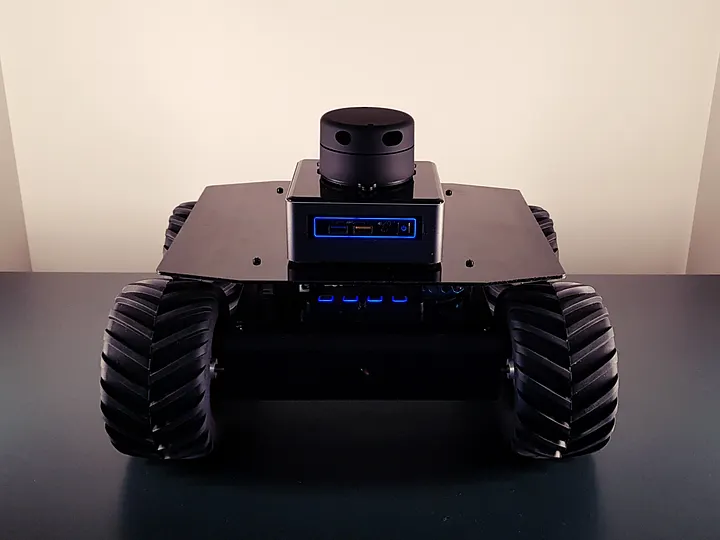
\includegraphics[width=0.75\linewidth]{figures/photos/rudra_lidar_front.png}

\vspace{1cm}

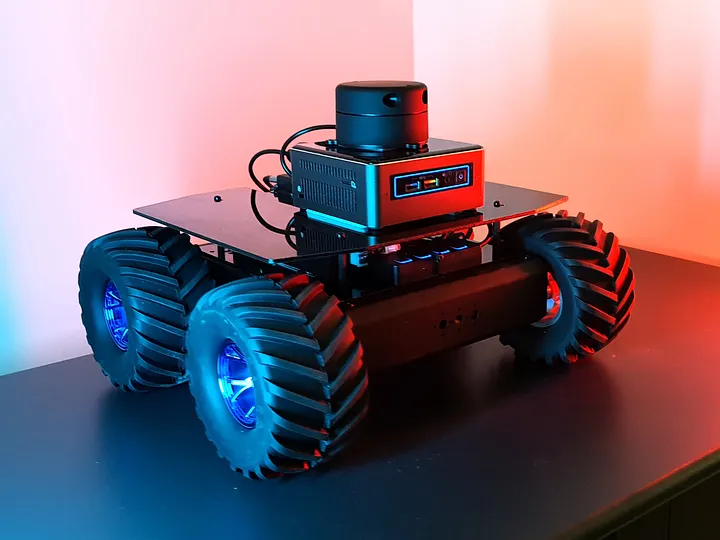
\includegraphics[width=0.75\linewidth]{figures/photos/rudra_finished_front.png}

\end{figure}
\clearpage

\chapter*{Preface}
\addcontentsline{toc}{chapter}{Preface}

This manual is written as the engineering development successor to the earlier \emph{\href{https://adarsh-gouda.medium.com/rudra-8e643e279d95?postPublishedType=repub}{Invoking the RUDRA}} article. The intent is to capture how \RUDRAv{} works as a complete robot system: why the hardware is split the way it is, how the ROS graph carries commands and telemetry, what equations sit underneath the motion model, how the serial protocols protect the base, how the LiDAR guard filters motion, how localization is staged, and how an operator should launch and monitor the machine.

\RUDRAv{} is a ROS 2 migration and modernization of the original RUDRAv3 rover. The hardware philosophy is preserved: the robot remains a modular differential-drive rover with a PS2 wireless controller, Arduino Uno, Teensy, dual Sabertooth motor drivers, YDLIDAR, and a main onboard computer. The important hardware upgrade for this edition is that the robot computer is an Intel NUC, not a Jetson Nano. The NUC is powered through a Mini-Box DCDC-USB rail, and the present ROS integration monitors that rail instead of attempting to control the converter output from ROS.

\begin{designbox}{How to read this manual}
Read Chapters~1--3 first if you are new to the system. Read Chapters~4--5 before touching motion or power. Read Chapters~6--11 before changing firmware, serial packets, obstacle behavior, or localization. Chapter~12 is the operator launch chapter. Chapters~13--14 are the commissioning, fault isolation, and roadmap chapters.
\end{designbox}

The manual is intentionally explicit about commands, file paths, message names, launch files, and parameter names because those details are where robot bringup usually fails. It also contains equations and implementation logic because RUDRA is not just a collection of launch commands. It is a physical machine whose behavior is constrained by kinematics, serial timing, controller deadbands, power integrity, sensor frame alignment, and safety timeouts.

\begin{safetybox}{Safety First}
Treat every software change as a potential motor command change. Lift the wheels or remove motor power for the first test after any firmware, serial, launch, or bridge modification. The NUC, Uno, Teensy, LiDAR, and ROS graph can be debugged without allowing the drive wheels to move.
\end{safetybox}

\tableofcontents
\listoffigures
\listoftables

\mainmatter
\chapter{System Intent and Development Philosophy}
\chapterquote{RUDRA is best understood as a layered robot, not as a single program. Each layer has one job and one failure boundary.}{Engineering principle for RUDRAv4}

\section{What RUDRAv4 is}

\RUDRAv{} is a four-wheel rover that uses differential-drive control. It accepts operator commands from a wireless PS2 controller and accepts ROS velocity commands through \topic{/cmd_vel}. It drives four DC motors through two Sabertooth motor controllers. It senses the surrounding space through a YDLIDAR and publishes robot telemetry into ROS 2 for monitoring, visualization, and eventual autonomous navigation.

The current architecture keeps the successful RUDRAv3 split-controller hardware model but replaces the old ROS 1 integration style with ROS 2 bridge nodes running on the NUC. Instead of pushing ROS directly into the microcontrollers, the NUC owns the ROS graph and the microcontrollers exchange compact plain-serial packets with it. This makes the system easier to debug because every boundary can be inspected with a serial terminal or a ROS topic echo.

\begin{figure}[htbp]
\centering
\resizebox{0.95\linewidth}{!}{\begin{tikzpicture}[node distance=9mm and 10mm, every node/.append style={font=\small}]
  \node[rudraHw,text width=24mm] (ps2) {PS2 wireless\\controller};
  \node[rudraHw,text width=24mm,right=of ps2] (uno) {Arduino Uno\\PS2 reader};
  \node[rudraBlock,text width=30mm,right=of uno] (nuc) {Intel NUC\\ROS~2 graph};
  \node[rudraHw,text width=24mm,right=of nuc] (teensy) {Teensy~4.1\\drive interface};
  \node[rudraHw,text width=26mm,right=of teensy] (sabers) {2x Sabertooth\\packet serial};
  \node[rudraHw,text width=20mm,right=of sabers] (motors) {4 drive\\motors};
  \node[rudraHw,text width=24mm,above=of nuc] (lidar) {YDLIDAR G2B\\LaserScan};
  \node[rudraHw,text width=28mm,below=of nuc] (dcdc) {DCDC-USB\\NUC power monitor};

  \draw[rudraArrow] (ps2) -- node[above=0.5]{\scriptsize wireless} (uno);
  \draw[rudraArrow] (uno) -- node[above=0.5]{\scriptsize \cmd{J,...}} (nuc);
  \draw[rudraArrow] (nuc) -- node[above=0.5]{\scriptsize \cmd{D,...}} (teensy);
  \draw[rudraArrow] (teensy) -- node[above=1]{\scriptsize 9600 baud} (sabers);
  \draw[rudraArrow] (sabers) -- (motors);
  \draw[rudraArrow] (lidar) -- node[right]{\scriptsize \topic{/scan}} (nuc);
  \draw[rudraDashed] (dcdc) -- node[right,align=center]{\scriptsize \topic{/rudra/}\\\scriptsize \topic{nuc_battery}} (nuc);
\end{tikzpicture}}
\caption{RUDRAv4 layered control architecture. ROS 2 lives on the NUC; the Uno, Teensy, and DCDC-USB remain hardware interface endpoints.}
\label{fig:system-layered}
\end{figure}

\section{The preserved design ideas}

The hardware baseline is intentionally familiar:

\begin{longtable}{p{0.28\linewidth}p{0.62\linewidth}}
\toprule
Element & Current role in RUDRAv4\\
\midrule
PS2 wireless controller & Human operator input for manual mode and obstacle-guard latch control.\\
Arduino Uno & Reads the PS2 receiver through the vendored PS2X library and publishes a compact serial joystick line.\\
Intel NUC & Runs Ubuntu, ROS 2 Lyrical, bridge nodes, LiDAR driver overlays, localization, RViz networking, and power diagnostics.\\
Teensy 4.1 & Receives final drive packets from the NUC and talks packet serial to both Sabertooth drivers. Optional firmware also emits IMU and wheel odometry telemetry.\\
Dual Sabertooth drivers & Drive the right and left motor sides through packet serial addresses 128 and 129.\\
YDLIDAR G2B & Publishes \topic{/scan} for obstacle guard, RViz, SLAM, and navigation experiments.\\
Mini-Box DCDC-USB & Regulates the dedicated NUC rail and exposes voltage/status telemetry over USB.\\
\bottomrule
\end{longtable}

\section{What changed from the older article}

The older RUDRA article mixed ROS 1, Jetson/Nano discussion, rosserial considerations, and the original firmware strategy. This edition keeps the engineering depth but changes the assumptions to match the current workspace:

\begin{itemize}
  \item The onboard computer is the NUC named \cmd{rudra}; the laptop station is \cmd{aghora}.
  \item The ROS stack is ROS 2 Lyrical and is sourced from \filep{/opt/ros/lyrical/setup.bash}.
  \item The robot workspace is \filep{/home/rudra/Projects/RUDRAv4}.
  \item The YDLIDAR SDK and driver are built in an external overlay at \filep{/home/rudra/ros2_ws}.
  \item The microcontrollers use plain serial instead of ROS serial. The plain serial boundary is deliberately simpler: \cmd{J,...} from Uno to NUC and \cmd{D,...} from NUC to Teensy.
  \item DCDC-USB is not treated as a motor-power device. It is the NUC power rail and is monitored through ROS diagnostics.
\end{itemize}

\section{System-of-systems view}

A rover that moves safely has at least five independent loops:

\begin{enumerate}
  \item \textbf{Human command loop}: PS2 controller to Uno to NUC.
  \item \textbf{Drive command loop}: NUC to Teensy to Sabertooth to motors.
  \item \textbf{Perception loop}: LiDAR to \topic{/scan} to obstacle guard and RViz.
  \item \textbf{State-estimation loop}: encoders and IMU to wheel odometry, raw IMU, EKF, and transforms.
  \item \textbf{Power-health loop}: DCDC-USB voltage readings to battery state and diagnostics.
\end{enumerate}

The important design choice is that the loops are coupled only at intentional points. LiDAR does not directly control the Sabertooth. It modifies the final forward command inside a ROS node. The DCDC monitor does not control the drivetrain. It publishes diagnostics. The Uno does not know about LiDAR. It only sends joystick state and the guard latch. This separation makes RUDRAv4 easier to test, easier to explain, and safer to develop.

\begin{figure}[htbp]
\centering
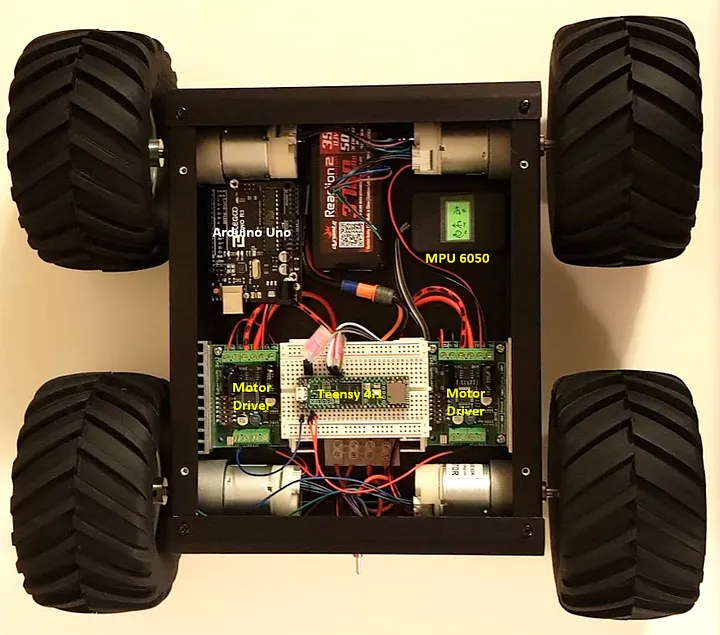
\includegraphics[width=0.72\linewidth]{figures/photos/rudra_chassis_top.png}
\caption{RUDRA chassis and internal electronics. This manual keeps the same modular hardware intent while documenting the current NUC-based RUDRAv4 software stack.}
\end{figure}

\section{Definition of done for the base platform}

For RUDRAv4, a base-control build is considered healthy when the following are all true:

\begin{itemize}
  \item \topic{/rudra/ps2_raw} updates at approximately controller-loop rate when the PS2 controller is active.
  \item \topic{/rudra/drive_cmd} shows only bounded \cmd{D,left,right,enable} lines.
  \item \topic{/rudra/teensy_ack} confirms that the Teensy receives those lines.
  \item \topic{/scan} publishes with frame \cmd{laser} after the YDLIDAR driver starts.
  \item \topic{/rudra/obstacle_guard} changes between clear, slowing, blocked, reverse/turn, disabled, or no-fresh-scan states as expected.
  \item \topic{/rudra/imu/raw}, \topic{/rudra/wheel_odom}, and \topic{/odometry/filtered} publish when localization firmware and launch are used.
  \item \topic{/rudra/nuc_battery} and \topic{/diagnostics} publish when the DCDC monitor is enabled.
  \item RViz on Aghora can view scan, marker, odometry, and transforms on the same DDS domain as Rudra.
\end{itemize}

\chapter{Hardware Architecture}

\section{Hardware inventory}

The current RUDRAv4 hardware is a modular base-control stack. The NUC is the central computer, but the low-level I/O remains distributed so that each device does what it is good at.

\begin{longtable}{p{0.22\linewidth}p{0.20\linewidth}p{0.48\linewidth}}
\toprule
Hardware & Interface to NUC or base & Engineering role\\
\midrule
Intel NUC & USB, Ethernet/Wi-Fi, DC input & Runs Ubuntu, ROS 2, launch files, bridge nodes, LiDAR driver overlays, monitoring, and development tools.\\
Mini-Box DCDC-USB & DC input/output and USB status & Regulates the NUC power rail and exposes voltage/status telemetry.\\
Arduino Uno & USB serial at 115200 baud & Reads PS2 receiver and publishes joystick packets.\\
PS2 controller/receiver & PS2X digital pins to Uno & Wireless manual driving and guard latch control.\\
Teensy 4.1 & USB serial at 115200 baud; Serial1 packet serial at 9600 baud & Converts NUC drive packets into Sabertooth packet serial and optional IMU/odometry telemetry.\\
Two Sabertooth drivers & Single-wire packet serial from Teensy TX1 & Right side address 128, left side address 129. Drives four motors as two differential sides.\\
YDLIDAR G2B & CP2102 USB serial adapter & Publishes 360-degree planar laser scans for obstacle guard and future SLAM.\\
MPU6050 & I2C to Teensy & Raw acceleration and gyro telemetry for localization experiments.\\
Wheel encoders & Interrupt pins to Teensy & Wheel-speed and odometry telemetry.\\
\bottomrule
\end{longtable}

\section{Physical and logical separation}

The architecture deliberately separates four domains:

\begin{enumerate}
  \item \textbf{Human input}: the PS2 receiver is on the Uno. If controller code changes, the Teensy motor driver firmware does not need to change.
  \item \textbf{Drive actuation}: the Teensy owns packet serial to the Sabertooths. The NUC never talks directly to the Sabertooth bus.
  \item \textbf{ROS intelligence}: the NUC owns topics, launch files, parameters, LiDAR processing, localization, and logging.
  \item \textbf{Power health}: DCDC-USB is monitored independently from the drivetrain power path.
\end{enumerate}

\begin{figure}[htbp]
\centering
\resizebox{0.98\linewidth}{!}{\begin{tikzpicture}[node distance=7mm and 10mm]
\node[rudraHw] (controller) {PS2\\controller};
\node[rudraHw,right=of controller] (receiver) {PS2 receiver\\to Uno pins};
\node[rudraHw,right=of receiver] (uno) {Arduino Uno\\PS2X};
\node[rudraBlock,right=of uno] (ros) {NUC ROS 2\\bridges};
\node[rudraHw,right=of ros] (teensy) {Teensy 4.1\\Serial1 TX};
\node[rudraHw,above right=of teensy] (right) {Right\\Sabertooth\\addr 128};
\node[rudraHw,below right=of teensy] (left) {Left\\Sabertooth\\addr 129};
\node[rudraHw,right=of right] (rm) {right motors};
\node[rudraHw,right=of left] (lm) {left motors};
\draw[rudraArrow] (controller) -- (receiver);
\draw[rudraArrow] (receiver) -- (uno);
\draw[rudraArrow] (uno) -- node[above=0.5]{USB \cmd{J,...}} (ros);
\draw[rudraArrow] (ros) -- node[above=0.5]{USB \cmd{D,...}} (teensy);
\draw[rudraArrow] (teensy) -- node[above=0.5,sloped]{packet serial} (right);
\draw[rudraArrow] (teensy) -- node[below=0.5,sloped]{same bus} (left);
\draw[rudraArrow] (right) -- (rm);
\draw[rudraArrow] (left) -- (lm);
\end{tikzpicture}}
\caption{RUDRAv4 hardware command chain from operator input to motor actuation.}
\end{figure}

\section{Known pin and address conventions}

The PS2 receiver remains wired to the Uno with the validated pinout:

\begin{center}
\begin{tabular}{lc}
\toprule
PS2 signal & Uno pin\\
\midrule
CLK & 9\\
CMD & 7\\
ATT & 6\\
DAT & 8\\
\bottomrule
\end{tabular}
\end{center}

The Sabertooth packet serial convention is:

\begin{center}
\begin{tabular}{lc}
\toprule
Device & Value\\
\midrule
Right Sabertooth address & 128\\
Left Sabertooth address & 129\\
Sabertooth packet serial baud & 9600\\
Teensy serial port to Sabertooth & \cmd{Serial1/TX1}\\
Command range & -127 to +127\\
\bottomrule
\end{tabular}
\end{center}

\begin{figure}[htbp]
\centering
\begin{subfigure}{0.46\linewidth}
\centering
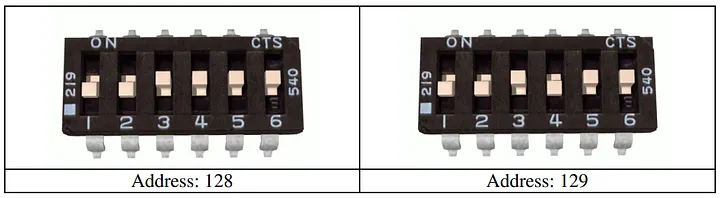
\includegraphics[width=\linewidth]{figures/photos/sabertooth_addresses_legacy.png}
\caption{Address convention retained from the previous hardware stack.}
\end{subfigure}\hfill
\begin{subfigure}{0.46\linewidth}
\centering
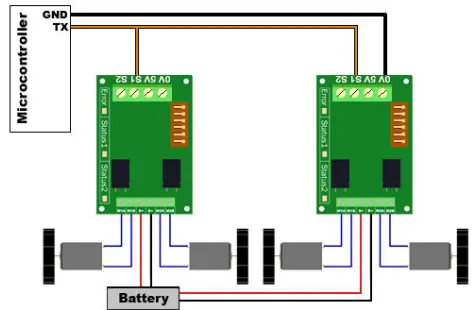
\includegraphics[width=\linewidth]{figures/photos/sabertooth_wiring_legacy.png}
\caption{Legacy Sabertooth wiring reference. Validate against the live robot before rewiring.}
\end{subfigure}
\caption{Sabertooth references retained as visual aids. RUDRAv4 uses the same addresses and single-wire packet serial principle.}
\end{figure}

\section{Why the NUC belongs at the center}

The NUC is the right place for ROS 2 because it can run the full graph, DDS discovery, LiDAR drivers, RViz networking, Python nodes, launch files, logging, and development tools. It also avoids tying robot software to microcontroller memory constraints. The microcontrollers remain excellent for deterministic low-level I/O. The NUC remains excellent for orchestration.

A practical rule follows:

\begin{operatorbox}{NUC vs. microcontroller responsibility rule}
Use the NUC for decisions that need ROS messages, parameters, launch files, sensor fusion, visualization, logs, or networking. Use the Teensy for packet serial timing, motor command ramping, encoder counting, IMU reading, and immediate command timeout. Use the Uno only for the PS2 receiver and compact joystick packet.
\end{operatorbox}

\section{USB device identity}

The robot should use persistent \filep{/dev/serial/by-id/...} device names, not short names like \filep{/dev/ttyACM0} or \filep{/dev/ttyUSB0}. Short names are assigned by probe order and can change after replugging, booting, or adding a device. Persistent names encode the USB device identity and are more stable.

Current stable paths in the workspace configuration are:

\begin{longtable}{p{0.18\linewidth}p{0.62\linewidth}p{0.13\linewidth}}
\toprule
Device & Preferred path & Typical short path\\
\midrule
Arduino Uno & \filep{/dev/serial/by-id/usb-Arduino__www.arduino.cc__0043_959313232323510182C0-if00} & \filep{/dev/ttyACM1}\\
Teensy 4.1 & \filep{/dev/serial/by-id/usb-Teensyduino_USB_Serial_9210670-if00} & \filep{/dev/ttyACM0}\\
YDLIDAR CP2102 & \filep{/dev/serial/by-id/usb-Silicon_Labs_CP2102_USB_to_UART_Bridge_Controller_0001-if00-port0} & \filep{/dev/ttyUSB0}\\
\bottomrule
\end{longtable}

Use the checked-in helper:

\begin{lstlisting}[language=bash]
cd /home/rudra/Projects/RUDRAv4
bash scripts/list_serial.sh
\end{lstlisting}

\section{Mechanical assumptions needed by software}

The software presently carries two key geometric constants from the older RUDRA design:

\begin{align}
R &= 0.0675\ \text{m} && \text{wheel radius reference},\\
L &= 0.29\ \text{m} && \text{wheelbase / track-width reference for differential motion}.
\end{align}

These values appear in the differential-drive equations, \cmd{/cmd_vel} conversion, and wheel odometry. If the physical wheel radius or track width changes, the firmware and ROS configuration must be updated together. A mismatched radius causes speed scale error. A mismatched track width causes yaw-rate error.

\chapter{ROS 2 Foundation for RUDRA}

\section{Why ROS 2 is the robot backbone}

\ros{} is not just a collection of libraries. In RUDRAv4 it is the distributed communication fabric that lets the NUC combine human input, motor command generation, LiDAR scans, state estimation, diagnostics, and remote visualization. The NUC runs nodes. Nodes communicate through topics and services. Launch files describe which nodes start together. YAML files store runtime parameters. DDS discovery allows Rudra and Aghora to see each other when they share the same domain.

The essential idea is that each robot function becomes a node with a clear interface. A node does not need to know how the other node is implemented. It needs only the message type and topic name.

\begin{figure}[htbp]
\centering
\resizebox{0.98\linewidth}{!}{\begin{tikzpicture}[node distance=8mm and 10mm]
\node[rudraBlock] (ps2) {\pkg{ps2_uno_to_teensy}};
\node[rudraBlock,right=of ps2] (guard) {\pkg{LidarObstacleGuard}\\inside bridge};
\node[rudraBlock,right=of guard] (teensy) {Teensy serial\\writer};
\node[rudraTopic,above=of ps2] (raw) {\topic{/rudra/ps2_raw}};
\node[rudraTopic,below=of ps2] (cmdvel) {\topic{/cmd_vel}};
\node[rudraTopic,above=of guard] (scan) {\topic{/scan}};
\node[rudraTopic,below=of guard] (status) {\topic{/rudra/obstacle_guard}};
\node[rudraTopic,above=of teensy] (drive) {\topic{/rudra/drive_cmd}};
\node[rudraTopic,below=of teensy] (ack) {\topic{/rudra/teensy_ack}};
\draw[rudraArrow] (ps2) -- (guard);
\draw[rudraArrow] (guard) -- (teensy);
\draw[rudraDashed] (ps2) -- (raw);
\draw[rudraDashed] (ps2) -- (cmdvel);
\draw[rudraArrow] (scan) -- (guard);
\draw[rudraDashed] (guard) -- (status);
\draw[rudraDashed] (teensy) -- (drive);
\draw[rudraDashed] (teensy) -- (ack);
\end{tikzpicture}}
\caption{ROS graph concept for manual driving. The node reads serial, publishes observability topics, applies LiDAR filtering, and writes final drive packets.}
\end{figure}

\section{Nodes, topics, messages, and parameters}

For RUDRAv4, the following ROS 2 terms are operationally important:

\begin{description}
  \item[Node] A running process or object that participates in ROS. Examples include \pkg{ps2_uno_to_teensy}, \pkg{cmd_vel_to_teensy}, \pkg{ydlidar_ros2_driver_node}, \pkg{ekf_filter_node}, and \pkg{dcdc_usb_monitor}.
  \item[Topic] A named stream of messages. Examples are \topic{/scan}, \topic{/cmd_vel}, \topic{/rudra/drive_cmd}, \topic{/rudra/wheel_odom}, and \topic{/diagnostics}.
  \item[Message type] The schema for a topic. \topic{/cmd_vel} uses \cmd{geometry_msgs/msg/Twist}. \topic{/scan} uses \cmd{sensor_msgs/msg/LaserScan}. \topic{/rudra/wheel_odom} uses \cmd{nav_msgs/msg/Odometry}.
  \item[Parameter] Runtime configuration loaded into a node. Serial ports, baud rates, stop distances, frame names, timeouts, and battery thresholds are parameters.
  \item[Launch file] A Python file that instantiates nodes with arguments, parameters, and optional includes.
\end{description}

\section{Workspace overlays}

RUDRAv4 uses an overlay chain. The order matters because later workspaces extend the environment created by earlier workspaces:

\begin{lstlisting}[language=bash]
source /opt/ros/lyrical/setup.bash
source /home/rudra/ros2_ws/install/setup.bash
source /home/rudra/Projects/RUDRAv4/install/setup.bash
\end{lstlisting}

The base ROS installation defines ROS 2 commands and core packages. The external workspace defines the YDLIDAR SDK and driver. The robot workspace defines \pkg{rudra_base_bridge}. If the LiDAR workspace is not sourced, ROS may still see the RUDRA bridge package but fail to find \pkg{ydlidar_ros2_driver}.

\section{DDS domain and remote visualization}

Rudra and Aghora must share a ROS domain to see each other. The helper scripts default to:

\begin{lstlisting}[language=bash]
export ROS_DOMAIN_ID=42
export ROS_LOCALHOST_ONLY=0
\end{lstlisting}

\cmd{ROS_DOMAIN_ID} separates independent ROS graphs on the same network. \cmd{ROS_LOCALHOST_ONLY=0} permits network discovery beyond the local machine. A common failure is that nodes are healthy on Rudra but Aghora sees nothing because the laptop is in a different domain or locked to localhost.

\section{Package structure}

The active robot package is \pkg{rudra_base_bridge}. Its development responsibilities are grouped as follows:

\begin{longtable}{p{0.30\linewidth}p{0.60\linewidth}}
\toprule
Path & Meaning\\
\midrule
\filep{config/rudra_v4_hardware.yaml} & Serial ports, robot constants, obstacle guard parameters, DCDC thresholds.\\
\filep{config/ydlidar_g2b.yaml} & YDLIDAR serial, frame, scan, intensity, frequency, range limits.\\
\filep{config/localization_ekf.yaml} & EKF inputs, frame names, two-dimensional mode, selected state variables.\\
\filep{launch/*.launch.py} & System bringup recipes.\\
\filep{rudra_base_bridge/*.py} & Python ROS 2 nodes and helper modules.\\
\filep{firmware/*/*.ino} & Uno and Teensy firmware sketches.\\
\filep{scripts/*.sh} & Operator wrappers that source the correct overlays and launch common modes.\\
\bottomrule
\end{longtable}

\section{ROS 2 mental model for RUDRA development}

When debugging, do not start by reading every file. Ask which boundary failed:

\begin{enumerate}
  \item Is the USB serial device visible at \filep{/dev/serial/by-id}? If not, the fault is below ROS.
  \item Is the node running? Use \cmd{ros2 node list}.
  \item Is the topic present? Use \cmd{ros2 topic list}.
  \item Is data arriving? Use \cmd{ros2 topic echo --once TOPIC}.
  \item Is the message frame correct? Use RViz, \cmd{ros2 topic echo}, and TF tools.
  \item Is a launch or parameter mistake causing a healthy node to use the wrong port, frame, or threshold?
\end{enumerate}

This is why the bridge nodes publish observability topics. The serial boundary is opaque unless you publish what was read and what was written. RUDRAv4 publishes \topic{/rudra/ps2_raw}, \topic{/rudra/drive_cmd}, \topic{/rudra/teensy_ack}, and \topic{/rudra/obstacle_guard} specifically to make that boundary visible.


\chapter{Fresh Ubuntu Setup for Rudra and Aghora}
\label{chap:fresh-setup}

\chapterquote{A robot workspace is only useful when a clean machine can be rebuilt into the same robot again. This chapter is the rebuild contract for the onboard NUC and the workstation.}{RUDRAv4 setup principle}

This chapter turns a fresh Ubuntu installation into a working two-machine \RUDRAv{} development system.  The robot computer is the Intel NUC mounted on the rover and named \cmd{rudra}.  The workstation laptop is named \cmd{aghora}.  Both machines run Ubuntu 26.04 and \ros{} Lyrical, but they have different jobs.  The NUC owns hardware, serial devices, the LiDAR driver, the Teensy bridge, DCDC monitoring, and launch files that move the robot.  Aghora is the engineering workstation: editing, Git, RViz, plotting, bag review, SLAM visualization, and remote operation.

\begin{designbox}{Outcome of the setup}
After this setup, opening a terminal on either machine should show a sourced \ros{} Lyrical environment, a consistent \cmd{ROS_DOMAIN_ID}, and the ability to build the RUDRAv4 workspace.  On \cmd{rudra}, hardware devices should appear under \filep{/dev/serial/by-id}.  On \cmd{aghora}, RViz should discover topics published by the NUC over the robot network.
\end{designbox}

\section{Machine roles}
\begin{table}[h]
\centering
\caption{Two-machine division of responsibility after a fresh install.}
\begin{tabularx}{\linewidth}{p{0.17\linewidth}p{0.28\linewidth}Y}
\toprule
Machine & Identity & Main responsibility \\
\midrule
\cmd{rudra} & Intel NUC7i7BNH on the rover & Hardware-facing \ros{} nodes: Uno bridge, Teensy bridge, LiDAR, obstacle guard, localization, DCDC-USB monitor, logs, and command safety. \\
\cmd{aghora} & Ubuntu workstation/laptop & Development, SSH access, Git, RViz, map building, launch observation, bag analysis, and remote visualization. \\
\bottomrule
\end{tabularx}
\end{table}

Both machines should use the same \cmd{ROS_DOMAIN_ID}.  RUDRAv4 uses \cmd{42} in the current workspace.  A mismatched DDS domain is the most common reason the laptop sees no topics even when both computers are healthy.

\section{Install Ubuntu 26.04}
Install Ubuntu 26.04 on both computers.  The NUC can run Desktop or Server; Desktop is more convenient during development because Arduino IDE, RViz, and VS Code are available locally.  The workstation should use Desktop.

Set the hostnames immediately after the first boot:

\begin{lstlisting}[language=bash,caption={Hostname setup on the NUC.}]
sudo hostnamectl set-hostname rudra
hostnamectl
cat /etc/hostname
\end{lstlisting}

\begin{lstlisting}[language=bash,caption={Hostname setup on the workstation.}]
sudo hostnamectl set-hostname aghora
hostnamectl
cat /etc/hostname
\end{lstlisting}

Update the base operating system on both machines:

\begin{lstlisting}[language=bash,caption={Base Ubuntu update.}]
sudo apt update
sudo apt upgrade -y
sudo apt install -y software-properties-common
sudo add-apt-repository universe
sudo reboot
\end{lstlisting}

\section{Bootstrap packages common to both machines}
The clean install should not assume build tools, Python headers, pip, venv, SSH, or network discovery tools are already present.  Install the common toolchain first:

\begin{lstlisting}[language=bash,caption={Common Linux development packages.}]
sudo apt update
sudo apt install -y \
  build-essential cmake pkg-config ninja-build \
  git curl wget gnupg ca-certificates lsb-release \
  locales software-properties-common \
  python3 python3-dev python3-pip python3-venv python3-setuptools python3-wheel \
  usbutils pciutils net-tools iproute2 udev \
  openssh-server avahi-daemon \
  terminator htop tree tmux unzip zip
\end{lstlisting}

Configure a UTF-8 locale before installing \ros{}:

\begin{lstlisting}[language=bash,caption={UTF-8 locale setup.}]
locale
sudo locale-gen en_US en_US.UTF-8
sudo update-locale LC_ALL=en_US.UTF-8 LANG=en_US.UTF-8
export LANG=en_US.UTF-8
locale
\end{lstlisting}

\section{Install ROS 2 Lyrical}
\ros{} Lyrical is the RUDRAv4 distribution for Ubuntu 26.04.  The official Lyrical installation page lists Ubuntu Resolute 26.04 as the binary package target.  Use the official ROS apt-source package rather than hand-written apt source lines because it avoids the signed-by conflicts that occur when old ROS source entries are left behind.

\begin{lstlisting}[language=bash,caption={Install the ROS apt source.}]
sudo apt update
sudo apt install -y curl
export ROS_APT_SOURCE_VERSION=$(curl -s https://api.github.com/repos/ros-infrastructure/ros-apt-source/releases/latest | grep -F "tag_name" | awk -F'"' '{print $4}')
curl -L -o /tmp/ros2-apt-source.deb \
  "https://github.com/ros-infrastructure/ros-apt-source/releases/download/${ROS_APT_SOURCE_VERSION}/ros2-apt-source_${ROS_APT_SOURCE_VERSION}.$(. /etc/os-release && echo ${UBUNTU_CODENAME:-${VERSION_CODENAME}})_all.deb"
sudo dpkg -i /tmp/ros2-apt-source.deb
\end{lstlisting}

Install the desktop distribution on both machines during development.  If the NUC must later be reduced, it can use \cmd{ros-lyrical-ros-base}, but Desktop is easier while bringing up a robot.

\begin{lstlisting}[language=bash,caption={Install ROS 2 Lyrical and core tools.}]
sudo apt update
sudo apt upgrade -y
sudo apt install -y \
  ros-lyrical-desktop \
  ros-dev-tools \
  python3-colcon-common-extensions \
  python3-rosdep \
  python3-vcstool
\end{lstlisting}

Install packages used by the current RUDRAv4 stack:

\begin{lstlisting}[language=bash,caption={RUDRAv4 ROS package set.}]
sudo apt install -y \
  ros-lyrical-rmw-fastrtps-cpp \
  ros-lyrical-rmw-cyclonedds-cpp \
  ros-lyrical-robot-state-publisher \
  ros-lyrical-joint-state-publisher-gui \
  ros-lyrical-xacro \
  ros-lyrical-tf2-tools \
  ros-lyrical-teleop-twist-keyboard \
  ros-lyrical-teleop-twist-joy \
  ros-lyrical-joy \
  ros-lyrical-joy-linux \
  ros-lyrical-imu-tools \
  ros-lyrical-imu-filter-madgwick \
  ros-lyrical-imu-complementary-filter \
  ros-lyrical-rviz-imu-plugin \
  ros-lyrical-robot-localization \
  diagnostic-updater \
  python3-serial \
  libcxx-serial-dev \
  libserialport-dev
\end{lstlisting}

Initialize rosdep:

\begin{lstlisting}[language=bash,caption={rosdep initialization.}]
sudo rosdep init || true
rosdep update
\end{lstlisting}

Verify ROS itself before cloning RUDRA:

\begin{lstlisting}[language=bash,caption={Basic ROS verification.}]
source /opt/ros/lyrical/setup.bash
echo "ROS_DISTRO=$ROS_DISTRO"
which ros2
ros2 doctor --report
\end{lstlisting}

\section{Clone and build the workspace}
On the NUC, the current workspace is:

\begin{lstlisting}[language=bash,caption={RUDRAv4 workspace path on the NUC.}]
mkdir -p /home/rudra/Projects
cd /home/rudra/Projects
git clone https://github.com/AdarshGouda/RUDRAv4.git
cd /home/rudra/Projects/RUDRAv4
\end{lstlisting}

On Aghora, use the same repository path when possible.  It keeps scripts, documentation, and local notes consistent:

\begin{lstlisting}[language=bash,caption={RUDRAv4 workspace path on Aghora.}]
mkdir -p ~/Projects
cd ~/Projects
git clone https://github.com/AdarshGouda/RUDRAv4.git
cd ~/Projects/RUDRAv4
\end{lstlisting}

Build the RUDRAv4 workspace:

\begin{lstlisting}[language=bash,caption={Build RUDRAv4.}]
cd /home/rudra/Projects/RUDRAv4
source /opt/ros/lyrical/setup.bash
rosdep install --from-paths src --ignore-src -r -y
colcon build --symlink-install
source install/setup.bash
ros2 pkg list | grep rudra
\end{lstlisting}

\section{Install serial permissions and board tools on the NUC}
The NUC opens three important USB serial devices: Arduino Uno, Teensy 4.1, and the CP2102 USB adapter used by the YDLIDAR.  Add the user to the serial groups and install udev rules before testing the robot.

\begin{lstlisting}[language=bash,caption={Serial permissions on the NUC.}]
sudo usermod -aG dialout,plugdev rudra
groups rudra
# Log out and back in after this step.
\end{lstlisting}

Install Teensy rules:

\begin{lstlisting}[language=bash,caption={Teensy udev rules.}]
curl -L -o /tmp/00-teensy.rules https://www.pjrc.com/teensy/00-teensy.rules
sudo install -m 0644 /tmp/00-teensy.rules /etc/udev/rules.d/00-teensy.rules
sudo udevadm control --reload-rules
sudo udevadm trigger
\end{lstlisting}

Install Arduino CLI and Teensy board support:

\begin{lstlisting}[language=bash,caption={Arduino CLI and Teensy board index.}]
sudo apt install -y arduino-cli
arduino-cli config init || true
arduino-cli config add board_manager.additional_urls https://www.pjrc.com/teensy/package_teensy_index.json
arduino-cli core update-index
arduino-cli core search teensy
\end{lstlisting}

Validate serial devices:

\begin{lstlisting}[language=bash,caption={Serial device identification.}]
cd /home/rudra/Projects/RUDRAv4
bash scripts/list_serial.sh
lsusb
ls -l /dev/serial/by-id
\end{lstlisting}

\section{Install the YDLIDAR external workspace on the NUC}
The current RUDRAv4 workspace treats the LiDAR driver as an external ROS workspace under \filep{/home/rudra/ros2_ws}.  Source order matters: base ROS, external LiDAR workspace, then RUDRAv4.

\begin{lstlisting}[language=bash,caption={Create the external LiDAR workspace.}]
mkdir -p /home/rudra/ros2_ws/src
cd /home/rudra/ros2_ws/src
git clone https://github.com/YDLIDAR/YDLidar-SDK.git
git clone -b humble https://github.com/YDLIDAR/ydlidar_ros2_driver.git
\end{lstlisting}

Build the SDK into the local external workspace rather than installing it globally:

\begin{lstlisting}[language=bash,caption={Build YDLidar-SDK locally.}]
cd /home/rudra/ros2_ws/src/YDLidar-SDK
mkdir -p build
cd build
cmake .. -DCMAKE_INSTALL_PREFIX=/home/rudra/ros2_ws/install/YDLidar-SDK
cmake --build .
cmake --install .
\end{lstlisting}

Build the ROS driver:

\begin{lstlisting}[language=bash,caption={Build YDLIDAR ROS 2 driver against the local SDK.}]
cd /home/rudra/ros2_ws
source /opt/ros/lyrical/setup.bash
export CMAKE_PREFIX_PATH=/home/rudra/ros2_ws/install/YDLidar-SDK:$CMAKE_PREFIX_PATH
colcon build --symlink-install --packages-select ydlidar_ros2_driver
source install/setup.bash
\end{lstlisting}

\section{Install the voice stack on the NUC}
\pkg{rudra_voice} needs a small Python environment that is separate from system Python but still able to see ROS Python packages. This is the fix for the \cmd{No module named 'sounddevice'} failure seen when ROS launches the node with the wrong interpreter.

Install audio and Python system dependencies:

\begin{lstlisting}[language=bash,caption={Voice OS dependencies.}]
sudo apt update
sudo apt install -y \
  alsa-utils espeak-ng \
  python3-venv python3-pip \
  libportaudio2 portaudio19-dev \
  curl wget unzip
\end{lstlisting}

Create the project voice virtual environment:

\begin{lstlisting}[language=bash,caption={Voice Python virtual environment.}]
cd /home/rudra/Projects/RUDRAv4
python3 -m venv --system-site-packages .venv_voice
source .venv_voice/bin/activate
python -m pip install --upgrade pip
python -m pip install vosk sounddevice numpy requests
python -c "import sounddevice, vosk, requests; print('voice python ok')"
\end{lstlisting}

\begin{designbox}{Why \cmd{--system-site-packages} is intentional}
ROS 2 Lyrical installs important Python modules through apt. The voice stack installs speech packages through pip. The \filep{.venv_voice} environment with \cmd{--system-site-packages} lets one Python interpreter see both worlds. If pip reports \cmd{externally-managed-environment}, pip is pointed at the system interpreter instead of \filep{.venv_voice}.
\end{designbox}

Download the Vosk speech-recognition model:

\begin{lstlisting}[language=bash,caption={Vosk model install.}]
mkdir -p /home/rudra/Projects/RUDRAv4/models
cd /home/rudra/Projects/RUDRAv4/models
wget https://alphacephei.com/vosk/models/vosk-model-small-en-us-0.15.zip
unzip vosk-model-small-en-us-0.15.zip
\end{lstlisting}

Install Piper locally for human-sounding offline speech. This keeps the install reproducible even when \cmd{sudo apt install piper} is not available or requires an interactive password:

\begin{lstlisting}[language=bash,caption={Local Piper install.}]
cd /home/rudra/Projects/RUDRAv4
mkdir -p tools/piper models/piper
curl -L --fail -o /tmp/piper_linux_x86_64.tar.gz \
  https://github.com/rhasspy/piper/releases/download/2023.11.14-2/piper_linux_x86_64.tar.gz
tar -xzf /tmp/piper_linux_x86_64.tar.gz -C tools/piper --strip-components=1
curl -L --fail -o models/piper/en_US-amy-medium.onnx \
  https://huggingface.co/rhasspy/piper-voices/resolve/main/en/en_US/amy/medium/en_US-amy-medium.onnx
curl -L --fail -o models/piper/en_US-amy-medium.onnx.json \
  https://huggingface.co/rhasspy/piper-voices/resolve/main/en/en_US/amy/medium/en_US-amy-medium.onnx.json
printf 'I am online. Ready for safe commands.\n' | \
  tools/piper/piper --model models/piper/en_US-amy-medium.onnx \
  --output_file /tmp/rudra_piper_test.wav
aplay /tmp/rudra_piper_test.wav
\end{lstlisting}

Check the P610 microphone and speakerphone:

\begin{lstlisting}[language=bash,caption={P610 audio check.}]
lsusb
arecord -l
aplay -l
arecord -f S16_LE -r 16000 -c 1 -d 5 /tmp/rudra_p610_test.wav
aplay /tmp/rudra_p610_test.wav
\end{lstlisting}

Ollama is optional. Install it only if natural-language routing is needed beyond deterministic commands. The full robot launch can start or check Ollama for you when \cmd{enable_ollama:=true}; the helper script below is also useful as a one-time readiness check after installation.

\begin{lstlisting}[language=bash,caption={Optional Ollama setup.}]
curl -fsSL https://ollama.com/install.sh | sh
bash /home/rudra/Projects/RUDRAv4/scripts/start_ollama.sh qwen2.5:3b
\end{lstlisting}

\section{Shell environment for every terminal}
Add the following block to \filep{~/.bashrc} on \cmd{rudra}.  On \cmd{aghora}, omit the external LiDAR workspace if it is not cloned locally.

\begin{lstlisting}[language=bash,caption={Recommended NUC bash environment.}]
# RUDRA ROS 2 environment
export RUDRA_WS="$HOME/Projects/RUDRAv4"
export RUDRA_LIDAR_WS="$HOME/ros2_ws"

if [ -f /opt/ros/lyrical/setup.bash ]; then
    source /opt/ros/lyrical/setup.bash
fi
if [ -f "$RUDRA_LIDAR_WS/install/setup.bash" ]; then
    source "$RUDRA_LIDAR_WS/install/setup.bash"
fi
if [ -f "$RUDRA_WS/install/setup.bash" ]; then
    source "$RUDRA_WS/install/setup.bash"
fi

export ROS_DOMAIN_ID=42
export ROS_LOCALHOST_ONLY=0
export ROS_AUTOMATIC_DISCOVERY_RANGE=SUBNET
export RMW_IMPLEMENTATION=rmw_fastrtps_cpp

alias rudra_ws='cd $RUDRA_WS'
alias cb='cd $RUDRA_WS && colcon build --symlink-install'
alias serialids='ls -l /dev/serial/by-id 2>/dev/null'
alias rosenv="printenv | grep -E 'ROS|RMW|RUDRA'"
printf '\n[RUDRA] ROS 2 Lyrical environment loaded. Workspace: %s\n' "$RUDRA_WS"
\end{lstlisting}

\section{SSH and network verification}
Enable SSH and mDNS on the NUC:

\begin{lstlisting}[language=bash,caption={NUC remote access.}]
sudo systemctl enable --now ssh
sudo systemctl enable --now avahi-daemon
hostname -I
systemctl status ssh --no-pager
\end{lstlisting}

From Aghora:

\begin{lstlisting}[language=bash,caption={SSH from Aghora to Rudra.}]
ssh rudra@rudra.local
\end{lstlisting}

Optional \filep{~/.ssh/config} entry on Aghora:

\begin{lstlisting}[caption={Aghora SSH shortcut.}]
Host rudra
    HostName rudra.local
    User rudra
    IdentityFile ~/.ssh/id_ed25519
\end{lstlisting}

Test ROS discovery.  On \cmd{rudra}:

\begin{lstlisting}[language=bash,caption={Publish a topic from the NUC.}]
source ~/.bashrc
ros2 run demo_nodes_cpp talker
\end{lstlisting}

On \cmd{aghora}:

\begin{lstlisting}[language=bash,caption={Listen from the workstation.}]
source ~/.bashrc
ros2 topic list
ros2 topic echo /chatter
\end{lstlisting}

\section{First clean-room bring-up checklist}
\begin{enumerate}
  \item Ubuntu updated on both machines.
  \item \cmd{rudra} and \cmd{aghora} hostnames set.
  \item \ros{} Lyrical installed and sourced on both machines.
  \item \cmd{ROS_DOMAIN_ID=42} on both machines.
  \item RUDRAv4 workspace cloned and built.
  \item \filep{.venv_voice} exists and \cmd{python -c "import sounddevice, vosk, requests"} succeeds inside it.
  \item Vosk model exists under \filep{models/vosk-model-small-en-us-0.15}.
  \item Piper binary exists at \filep{tools/piper/piper}; Piper test audio plays through \cmd{aplay}.
  \item \cmd{espeak-ng} is installed as the fallback speech output.
  \item NUC user belongs to \cmd{dialout} and \cmd{plugdev}.
  \item Teensy rules installed.
  \item \filep{/dev/serial/by-id} shows Uno, Teensy, and LiDAR adapter.
  \item Aghora can SSH into \cmd{rudra}.
  \item Aghora can see ROS topics from \cmd{rudra}.
\end{enumerate}

\section{First integrated launch after clean setup}
After the checklist passes, use the single full launch file:

\begin{lstlisting}[language=bash,caption={Integrated RUDRAv4 bringup on the NUC.}]
cd /home/rudra/Projects/RUDRAv4
source /opt/ros/lyrical/setup.bash
source /home/rudra/ros2_ws/install/setup.bash
source install/setup.bash
ros2 launch rudra_base_bridge rudra_full.launch.py
\end{lstlisting}

For the normal robot-mounted NUC, enable DCDC monitoring:

\begin{lstlisting}[language=bash,caption={Integrated launch with NUC power monitoring.}]
ros2 launch rudra_base_bridge rudra_full.launch.py enable_dcdc_monitor:=true
\end{lstlisting}

To let the voice stack use Ollama for uncertain phrases, opt in explicitly:

\begin{lstlisting}[language=bash,caption={Integrated launch with Ollama voice routing.}]
ros2 launch rudra_base_bridge rudra_full.launch.py \
  enable_dcdc_monitor:=true \
  enable_ollama:=true \
  voice_use_llm_router:=true
\end{lstlisting}

Expected early launch signs are: the launch prints the voice Python as \filep{.venv_voice/bin/python}, the P610 is detected by name, \topic{/scan} appears after the LiDAR finishes startup, \topic{/rudra/wheel_odom} and \topic{/rudra/imu/raw} publish from Teensy telemetry, \topic{/odometry/filtered} publishes from the EKF, and \topic{/rudra_voice/transcript} updates when speech is heard. The full launch keeps \cmd{voice_use_llm_router} off unless you turn it on, so deterministic voice commands work even if Ollama is stopped.

\begin{operatorbox}{First launch rule of thumb}
After a clean NUC install, use \cmd{ros2 launch rudra_base_bridge rudra_full.launch.py} as the main bringup command. Add launch arguments only for the capability being tested: \cmd{enable_dcdc_monitor:=true} for NUC power diagnostics, \cmd{enable_rviz:=true} for local visualization, and \cmd{enable_ollama:=true voice_use_llm_router:=true} for LLM-assisted voice phrases.
\end{operatorbox}

\begin{safetybox}{Do not test motion yet}
The purpose of this chapter is to rebuild the software platform.  Wheels should stay lifted or motor battery power should stay disconnected until the firmware and serial bridge chapters have been validated.
\end{safetybox}

\chapter{Differential-Drive Theory}

\section{Why RUDRA is a differential-drive robot}

RUDRA steers by commanding different speeds on the left and right sides. If both sides move forward at the same speed, the rover translates forward. If the right side is faster than the left, the rover turns left. If the two sides move in opposite directions, the rover spins about a point near its center.

\begin{figure}[htbp]
\centering
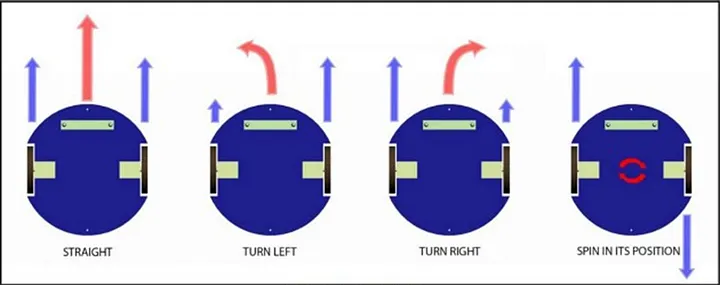
\includegraphics[width=0.72\linewidth]{figures/photos/differential_turn_modes_legacy.png}
\caption{Differential-drive motion modes: straight, turn, rotate, and spin-in-place behavior.}
\end{figure}

Although RUDRA has four wheels, the control abstraction is two-sided: a left virtual wheel and a right virtual wheel. Each virtual side represents the average ground speed of the two wheels on that side.

\section{Forward kinematics}

Let:

\begin{align*}
R &= \text{wheel radius},\\
L &= \text{distance between left and right wheel centerlines},\\
\omega_r &= \text{right wheel angular speed},\\
\omega_l &= \text{left wheel angular speed},\\
v &= \text{body forward speed},\\
\Omega &= \text{body yaw rate}.
\end{align*}

The wheel linear speeds are:

\begin{align}
v_r &= R\omega_r,\\
v_l &= R\omega_l.
\end{align}

The body forward speed and yaw rate are:

\begin{align}
v &= \frac{v_r+v_l}{2} = \frac{R}{2}(\omega_r+\omega_l), \label{eq:body-v}\\
\Omega &= \frac{v_r-v_l}{L} = \frac{R}{L}(\omega_r-\omega_l). \label{eq:body-w}
\end{align}

The planar pose is:

\begin{equation}
\mathbf{x}=\begin{bmatrix}x & y & \theta\end{bmatrix}^T.
\end{equation}

Its continuous-time derivative is:

\begin{equation}
\dot{\mathbf{x}} =
\begin{bmatrix}
\dot{x}\\ \dot{y}\\ \dot{\theta}
\end{bmatrix}
=
\begin{bmatrix}
v\cos\theta\\ v\sin\theta\\ \Omega
\end{bmatrix}.
\label{eq:pose-derivative}
\end{equation}

\section{Inverse kinematics}

ROS navigation and teleoperation commonly express a mobile-base command as \cmd{Twist}: linear velocity \(v\) and angular velocity \(\Omega\). RUDRA must convert that into side speeds:

\begin{align}
v_l &= v - \frac{\Omega L}{2}, \label{eq:left-side-speed}\\
v_r &= v + \frac{\Omega L}{2}. \label{eq:right-side-speed}
\end{align}

If wheel angular speeds are needed:

\begin{align}
\omega_l &= \frac{v_l}{R}=\frac{2v-\Omega L}{2R},\\
\omega_r &= \frac{v_r}{R}=\frac{2v+\Omega L}{2R}.
\end{align}

\begin{figure}[htbp]
\centering
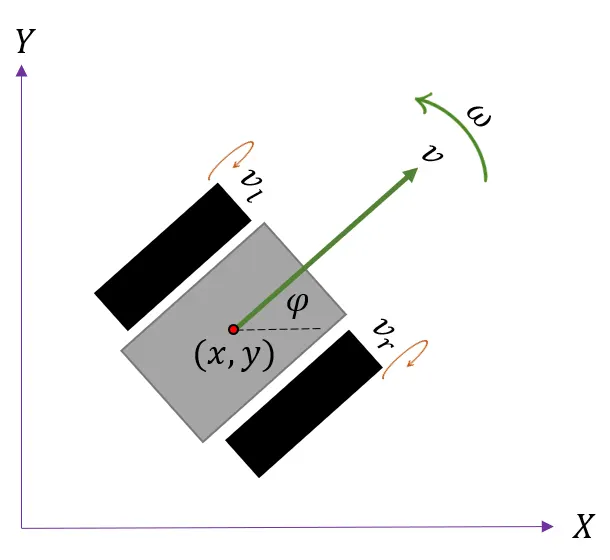
\includegraphics[width=0.55\linewidth]{figures/photos/diff_drive_frame_legacy.png}
\caption{Differential-drive coordinate frame and wheel-speed notation.}
\end{figure}

\section{Discrete odometry}

For telemetry, the Teensy can estimate wheel linear speed from encoder counts. If \(\Delta n\) counts are observed over \(\Delta t\), encoder counts per revolution are \(N\), and wheel radius is \(R\), then:

\begin{equation}
v_{wheel} = \frac{\Delta n}{N}\frac{2\pi R}{\Delta t}.
\label{eq:encoder-speed}
\end{equation}

RUDRAv4 firmware uses \(R=0.0675\) m, \(L=0.29\) m, and \(N=1683\) counts per revolution in the IMU/odometry Teensy sketch. Left and right side speeds are averaged from two encoders per side:

\begin{align}
v_l &= \frac{v_{L1}+v_{L2}}{2},\\
v_r &= \frac{v_{R1}+v_{R2}}{2}.
\end{align}

The firmware then computes:

\begin{align}
v_x &= \frac{v_l+v_r}{2},\\
\Omega_{enc} &= \frac{v_r-v_l}{L}.
\end{align}

For a sample period \(\Delta t\):

\begin{align}
\Delta \theta_{enc} &= \Omega_{enc}\Delta t,\\
\theta_k &= \theta_{k-1} + \Delta \theta,\\
x_k &= x_{k-1} + v_x\Delta t\cos(\theta_k),\\
y_k &= y_{k-1} + v_x\Delta t\sin(\theta_k).
\end{align}

The current firmware optionally blends encoder yaw increment and gyro yaw increment:

\begin{equation}
\Delta\theta = \alpha\Delta\theta_{enc} + (1-\alpha)\omega_{z,imu}\Delta t,
\end{equation}

where the present sketch uses \(\alpha=0.5\). This is a simple complementary blend in firmware; the ROS-side EKF is still the proper place to perform state estimation once the raw signals are stable.

\section{Command normalization to Sabertooth range}

The Teensy expects signed integer side commands:

\begin{equation}
u_l,u_r \in [-127,127].
\end{equation}

The \pkg{cmd_vel_to_teensy} bridge converts \topic{/cmd_vel} into side speeds and normalizes by the configured maximum linear speed:

\begin{align}
\tilde{u}_l &= \mathrm{sat}\left(\frac{v_l}{v_{max}},-1,1\right),\\
\tilde{u}_r &= \mathrm{sat}\left(\frac{v_r}{v_{max}},-1,1\right),\\
u_l &= \mathrm{round}(127\tilde{u}_l),\\
u_r &= \mathrm{round}(127\tilde{u}_r).
\end{align}

This is not closed-loop wheel-speed control. It is a bounded open-loop command mapping. The present design intentionally brings up serial, telemetry, LiDAR guard, and localization before adding wheel PID.

\section{Manual joystick mixing}

The PS2 bridge uses tank-style mixing from joystick throttle and steering:

\begin{align}
u_{throttle} &= f(\text{Ly}),\\
u_{steer} &= f(\text{Rx}),\\
u_l &= \mathrm{sat}(u_{throttle}-u_{steer}, -127, 127),\\
u_r &= \mathrm{sat}(u_{throttle}+u_{steer}, -127, 127).
\end{align}

The axis mapping function centers the raw PS2 value around 127, scales it by 127, applies a deadband, and clamps the result to the Sabertooth command range. The important practical consequence is that a noisy joystick center does not command motion.

\section{Why PID is not yet the first control problem}

A PID loop is useful only after the sensing and command chain is trustworthy. RUDRAv4 has the correct staging order:

\begin{enumerate}
  \item Verify PS2 packets and \topic{/cmd_vel} mapping.
  \item Verify Teensy drive packet acknowledgement and motor directions.
  \item Verify encoder sign, scale, and side assignment.
  \item Verify IMU scale and yaw sign.
  \item Verify odometry and TF consistency.
  \item Add PID only after the open-loop system is observable.
\end{enumerate}

A wheel PID loop would compare target wheel speed and measured wheel speed:

\begin{equation}
e(t)=v_{target}(t)-v_{measured}(t),
\end{equation}

and compute:

\begin{equation}
u(t)=K_p e(t)+K_i\int_0^t e(\tau)d\tau+K_d\frac{de(t)}{dt}.
\end{equation}

But if encoder polarity, CPR, radius, sample time, or side mapping is wrong, PID will hide or amplify the wrong problem. The current open-loop base is therefore the correct commissioning foundation.

\chapter{Power and Electrical Architecture}

\section{Power separation}

RUDRAv4 should be treated as two electrical systems sharing the robot chassis:

\begin{enumerate}
  \item \textbf{Drive power}: motor battery, Sabertooth motor drivers, and drive motors.
  \item \textbf{Compute power}: 4S LiPo, DCDC-USB, regulated NUC input, USB telemetry connection, and ROS diagnostics.
\end{enumerate}

The NUC rail must not be confused with the Sabertooth motor rail. The DCDC-USB integration is for powering and monitoring the NUC. It is not a drivetrain controller.

\begin{figure}[htbp]
\centering
\resizebox{0.85\linewidth}{!}{\begin{tikzpicture}[node distance=9mm and 12mm]
\node[rudraHw] (lipo) {4S LiPo\\16.8 V full\\14.8 V nominal};
\node[rudraHw,right=of lipo] (dcdc) {Mini-Box\\DCDC-USB};
\node[rudraHw,right=of dcdc] (nuc) {Intel NUC\\19 V input};
\node[rudraBlock,below=of dcdc] (mon) {\pkg{dcdc_usb_monitor}};
\node[rudraTopic,below=of mon] (topics) {\topic{/rudra/nuc_battery}\\\topic{/diagnostics}};
\node[rudraHw,above=of dcdc] (drive) {Separate drive battery\\to Sabertooths};
\draw[rudraArrow] (lipo) -- node[above=0.5]{DC in} (dcdc);
\draw[rudraArrow] (dcdc) -- node[above=0.5]{regulated output} (nuc);
\draw[rudraDashed] (dcdc) -- node[right]{USB status} (mon);
\draw[rudraDashed] (mon) -- (topics);
\draw[rudraArrow] (drive) -- ++(3,0) node[right]{motors};
\end{tikzpicture}}
\caption{DCDC-USB is the NUC rail monitor and regulator; drivetrain power remains a separate safety-critical path.}
\end{figure}

\section{NUC voltage tolerance}

The NUC rail is treated as a 19 V input with a \(\pm 10\%\) acceptable range:

\begin{align}
V_{min} &= 19(1-0.10)=17.1\ \text{V},\\
V_{max} &= 19(1+0.10)=20.9\ \text{V}.
\end{align}

The workspace configuration uses:

\begin{lstlisting}[language={},caption={DCDC output thresholds in hardware YAML}]
expected_output_min_voltage: 17.1
expected_output_max_voltage: 20.9
\end{lstlisting}

Before plugging the DCDC output into the NUC, measure the live output with a multimeter. A USB-only DCDC status reading can show a programmed target voltage even when the input/output power stage is not live.

\section{4S LiPo thresholds}

The current monitor configuration assumes a 4S LiPo pack. The important values are:

\begin{center}
\begin{tabular}{lcc}
\toprule
State & Pack voltage & Average cell voltage\\
\midrule
Full & 16.8 V & 4.20 V/cell\\
Nominal & 14.8 V & 3.70 V/cell\\
Warning & 14.4 V & 3.60 V/cell\\
Critical & 13.2 V & 3.30 V/cell\\
Optional shutdown threshold & 12.8 V & 3.20 V/cell\\
\bottomrule
\end{tabular}
\end{center}

The monitor estimates battery percentage linearly from input voltage:

\begin{equation}
\mathrm{SOC}_{est}=\mathrm{sat}\left(\frac{V_{in}-V_{empty}}{V_{full}-V_{empty}},0,1\right).
\end{equation}

This is a dashboard estimate, not a coulomb counter. LiPo voltage depends on load, temperature, internal resistance, and recovery after load removal.

\begin{figure}[htbp]
\centering
\resizebox{0.98\linewidth}{!}{\begin{tikzpicture}
\begin{axis}[
width=0.78\linewidth,height=6cm,
xlabel={4S LiPo input voltage (V)},ylabel={Estimated percentage},
xmin=12.6,xmax=17.0,ymin=0,ymax=1.05,grid=both,
legend pos=south east]
\addplot[thick,rudraTeal,domain=13.2:16.8,samples=2]{(x-13.2)/(16.8-13.2)};
\addplot[thick,rudraAmber,dashed] coordinates {(14.4,0) (14.4,1)};
\addplot[thick,black,dashed] coordinates {(13.2,0) (13.2,1)};
\legend{linear estimate, warning, critical}
\end{axis}
\end{tikzpicture}}
\caption{Linear state-of-charge estimate used for the NUC DCDC input monitor.}
\end{figure}

\section{DCDC-USB monitor behavior}

The ROS node \pkg{dcdc_usb_monitor} wraps the vendor command:

\begin{lstlisting}[language=bash]
dcdc-usb -a
\end{lstlisting}

It parses voltage and status fields, then publishes:

\begin{itemize}
  \item \topic{/rudra/nuc_battery} as \cmd{sensor_msgs/msg/BatteryState}
  \item \topic{/diagnostics} as \cmd{diagnostic_msgs/msg/DiagnosticArray}
\end{itemize}

The utility does not provide current, so the node cannot compute NUC power. Instead, it monitors input voltage, output voltage, programmed output, output enable state, and input voltage sag. Sag is a useful warning that the pack is weak, wiring resistance is high, or NUC load is unusually high.

\section{Monitor-first integration}

Automatic shutdown is available but intentionally disabled by default:

\begin{lstlisting}[language={}]
shutdown_enabled: false
shutdown_voltage: 12.8
shutdown_hold_sec: 5.0
shutdown_command: "sudo shutdown -h now"
\end{lstlisting}

Enable shutdown only after the DCDC readings are verified against a multimeter and the NUC has been tested under realistic load. Premature shutdown automation can be more disruptive than helpful during bringup.

\begin{safetybox}{Power-on validation}
Validate in three stages: USB-only DCDC communication, powered DCDC output without the NUC load, then NUC-powered integration with ROS monitoring. Do not skip the multimeter check between DCDC and NUC.
\end{safetybox}

\section{USB power caveats}

The Uno, Teensy, and YDLIDAR are USB devices from the NUC. The LiDAR can continue spinning if the USB port remains powered even after a driver process stops. The software can request driver shutdown, but it cannot remove physical USB power unless the hub or port supports that capability. If the LiDAR continues spinning after shutdown, unplug it or cut power at the USB hub.

The same practical rule applies to motor power: stopping ROS is not the same as disconnecting drive battery power. Keep a physical disconnect accessible during tests.


\chapter{Intel NUC7i7BNH and DCDC-USB}
\label{chap:nuc-dcdc}

The onboard computer is an Intel NUC7i7BNH.  In earlier RUDRA material the robot deck used a Jetson Nano.  RUDRAv4 now uses the NUC as the primary ROS computer, so the power architecture, runtime monitoring, shutdown policy, and mechanical mounting assumptions should be documented around the NUC.

\section{NUC role in the robot}
The NUC is not a microcontroller.  It is a Linux computer running \ros{}, launch files, Python bridge nodes, LiDAR drivers, RViz when needed, logging, and networking.  It should not directly toggle motor-driver pins or depend on real-time Linux timing for wheel safety.  The NUC sends commands to the Teensy; the Teensy owns the immediate motor-output timing and timeout behavior.

\begin{table}[h]
\centering
\caption{NUC responsibilities versus firmware responsibilities.}
\begin{tabularx}{\linewidth}{p{0.28\linewidth}Y}
\toprule
NUC responsibility & Firmware responsibility \\
\midrule
ROS graph, launch files, parameters, logs, SSH, RViz, LiDAR driver, DCDC monitor, obstacle guard, localization, command arbitration & Pin timing, PS2 electrical interface, MPU6050 I2C reads, encoder counting, packet serial to Sabertooth, immediate motor stop on missing command \\
\bottomrule
\end{tabularx}
\end{table}

\section{NUC7i7BNH electrical input}
The NUC is treated as a 19 V class load.  The current RUDRAv4 configuration monitors the DCDC output against a 19 V nominal rail with an accepted range of \SI{17.1}{\volt} to \SI{20.9}{\volt}.  That range is also encoded in \filep{src/rudra_base_bridge/config/rudra_v4_hardware.yaml}:

\begin{lstlisting}[caption={NUC DCDC output range from RUDRAv4 hardware config.}]
expected_output_min_voltage: 17.1
expected_output_max_voltage: 20.9
\end{lstlisting}

At power \(P\), output voltage \(V_o\), and DCDC efficiency \(\eta\), the battery input current is approximated by:
\begin{equation}
I_{in} \approx \frac{P}{\eta V_{in}}.
\end{equation}

This equation matters because the DCDC-USB status utility reports voltages and status fields, but not output current.  The monitor cannot compute watts directly.  Instead, RUDRAv4 watches input voltage, output voltage, programmed output voltage, and sudden input sag.

\section{DCDC-USB role}
The Mini-Box DCDC-USB is the regulated supply between the dedicated 4S NUC LiPo and the NUC DC input.  It provides a programmable output and a USB telemetry/configuration interface.  The robot wiring intent is:

\begin{center}
\resizebox{0.92\linewidth}{!}{%
\begin{tikzpicture}[node distance=16mm and 18mm, every node/.append style={font=\small}]
  \node[rudraHw, minimum width=30mm] (bat) {OVONIC 4S LiPo\\14.8 V nominal};
  \node[rudraBlock, right=of bat, minimum width=30mm] (dcdc) {Mini-Box\\DCDC-USB};
  \node[rudraHw, right=of dcdc, minimum width=34mm] (nuc) {Intel NUC7i7BNH\\ROS 2 computer};
  \node[rudraTopic, below=14mm of dcdc, minimum width=38mm] (usb) {USB telemetry\\\cmd{dcdc-usb -a}};
  \node[rudraBlock, right=of usb, minimum width=38mm] (mon) {ROS monitor\\\pkg{dcdc_usb_monitor}};
  \draw[rudraArrow] (bat) -- (dcdc);
  \draw[rudraArrow] (dcdc) -- (nuc);
  \draw[rudraDashed] (dcdc) -- (usb);
  \draw[rudraArrow] (usb) -- (mon);
  \node[font=\scriptsize, above=1mm of dcdc] {programmable 19 V class output};
  \node[font=\scriptsize, below=1mm of bat] {6-34 V DCDC input window};
\end{tikzpicture}}
\end{center}

The DCDC-USB does not power the Sabertooths and it does not command motors.  It is a dedicated NUC rail.

\section{Programming the DCDC-USB}
RUDRAv4 includes a source snapshot of the Mini-Box Linux utility under \filep{reference/DCDC/dcdc-usb}.  The current repo includes \filep{scripts/install_dcdc_usb_tool.sh}, which builds the tool, installs it, and adds a udev rule for the USB device.

\begin{lstlisting}[language=bash,caption={Install the DCDC-USB Linux utility from the RUDRAv4 workspace.}]
cd /home/rudra/Projects/RUDRAv4
bash scripts/install_dcdc_usb_tool.sh
\end{lstlisting}

Reconnect the USB cable and read the board:

\begin{lstlisting}[language=bash,caption={Read all DCDC-USB status fields.}]
dcdc-usb -a
\end{lstlisting}

The included utility readme states that running \cmd{dcdc-usb} with no parameters displays the current output voltage, \cmd{sudo dcdc-usb -a} displays all settings, and \cmd{sudo dcdc-usb -v 20.50} programs a \SI{20.5}{\volt} output.  For RUDRAv4, use a 19 V class setting and verify with a multimeter before connecting the NUC.

\begin{lstlisting}[language=bash,caption={Example: program a 19.6 V NUC output target.}]
# Bench only. Do not connect the NUC until the output is verified with a meter.
sudo dcdc-usb -v 19.60
sudo dcdc-usb -a
\end{lstlisting}

\begin{safetybox}{Programming is not verification}
A programmed target voltage is not the same as a verified live output.  Before plugging the DCDC output into the NUC, power the DCDC input from the 4S LiPo and measure the DCDC output with a multimeter under a safe no-NUC condition.
\end{safetybox}

\section{Interpreting DCDC-USB output}
The status output can contain two separate output-voltage meanings: a live output reading and a programmed target.  The RUDRAv4 parser preserves this distinction.  If the board is connected only over USB but the LiPo input is absent, it is possible to see \cmd{input voltage: 0.00} and a programmed target field.  That does not mean the NUC rail is powered.

\begin{lstlisting}[caption={Typical status fields used by RUDRAv4.}]
input voltage: 15.42
output voltage: 19.40
mode: 0 (dumb)
output enable: On
\end{lstlisting}

The ROS node parses these fields into \topic{/rudra/nuc_battery} and \topic{/diagnostics}.  It estimates state of charge from pack voltage only:
\begin{equation}
\mathrm{SOC}_{est}=\mathrm{clip}\left(\frac{V_{in}-V_{empty}}{V_{full}-V_{empty}},0,1\right).
\end{equation}

Because LiPo voltage sags under load, \(\mathrm{SOC}_{est}\) is a dashboard hint, not a precision fuel gauge.

\section{ROS monitor}
Run the DCDC monitor alone:

\begin{lstlisting}[language=bash,caption={Launch the standalone DCDC monitor.}]
cd /home/rudra/Projects/RUDRAv4
source /opt/ros/lyrical/setup.bash
source install/setup.bash
ros2 launch rudra_base_bridge dcdc_usb_monitor.launch.py
\end{lstlisting}

Monitor topics:

\begin{lstlisting}[language=bash,caption={DCDC monitor topics.}]
ros2 topic echo /rudra/nuc_battery
ros2 topic echo /diagnostics
\end{lstlisting}

The node publishes \topic{/rudra/nuc_battery} as \cmd{sensor_msgs/msg/BatteryState}.  Since the DCDC-USB utility does not report output current, \cmd{current}, \cmd{charge}, \cmd{capacity}, and \cmd{design_capacity} are intentionally unknown.  The voltage fields and diagnostic message are the useful signals.

\section{Shutdown policy}
The configuration contains warning, critical, and shutdown thresholds for the NUC 4S input pack:

\begin{lstlisting}[caption={DCDC monitor safety thresholds.}]
full_voltage: 16.8
empty_voltage: 13.2
warning_voltage: 14.4
critical_voltage: 13.2
shutdown_voltage: 12.8
shutdown_enabled: false
shutdown_hold_sec: 5.0
\end{lstlisting}

Leave shutdown disabled until the DCDC telemetry agrees with a multimeter and the NUC runtime has been tested.  After validation, enabling shutdown can protect the filesystem from brownout, but it must not surprise an operator during bench testing.

\section{Bench validation sequence}
\begin{enumerate}
  \item USB-only test: connect the DCDC-USB to the NUC over USB and verify \cmd{dcdc-usb -a} can communicate.
  \item Programming test: set the 19 V class output target with \cmd{sudo dcdc-usb -v 19.60}.
  \item Powered no-load test: connect the 4S LiPo to the DCDC input, leave the NUC output disconnected, and verify output with a multimeter.
  \item Loaded bench test: power the NUC from the DCDC output while still on the bench.  Run \cmd{dcdc-usb -a} and \topic{/rudra/nuc_battery}.
  \item Robot test: route wiring cleanly, strain-relieve the barrel output, and confirm the NUC does not reboot during LiDAR startup.
\end{enumerate}


\chapter{Sabertooth Motor Driver System}
\label{chap:sabertooth}

RUDRAv4 uses two Dimension Engineering Sabertooth dual regenerative motor drivers.  Each driver controls two brushed DC motors, so two boards support the four-wheel differential-drive base.  The RUDRA design uses packetized serial from the Teensy to the Sabertooths rather than direct PWM from the NUC.

\begin{figure}[h]
\centering
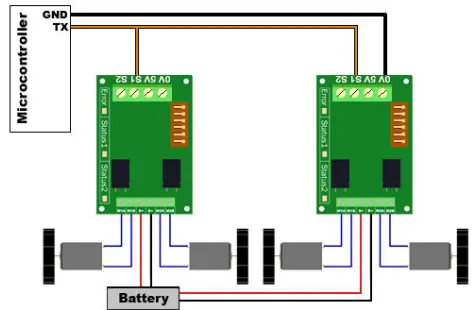
\includegraphics[width=0.92\linewidth]{figures/photos/sabertooth_wiring_article.png}
\caption{Sabertooth motor-driver wiring concept preserved from the RUDRA article assets.}
\end{figure}

\section{Why the Sabertooth is used}
A small H-bridge module can spin a motor on a bench, but RUDRA needs a driver that can tolerate real robot loads, regenerative events, bidirectional drive, and differential steering.  The Sabertooth 2x12 class driver is designed for medium robots and supports multiple control modes, including serial and packetized serial.  In RUDRAv4, packetized serial keeps the wiring simple: one Teensy serial bus can command both motor-controller addresses.

\section{Addressing model}
The current RUDRAv4 firmware contract uses:

\begin{lstlisting}[caption={Sabertooth address contract.}]
Right Sabertooth address: 128
Left  Sabertooth address: 129
Packet serial baud:       9600
Motor command range:      -127 to +127
\end{lstlisting}

The Teensy is the only board that talks packet serial to the Sabertooths.  The NUC sends high-level drive commands to the Teensy; the Teensy converts those commands into Sabertooth packet serial.

\begin{figure}[htbp]
\centering
\resizebox{0.92\linewidth}{!}{%
\begin{tikzpicture}[node distance=8mm and 11mm, every node/.append style={font=\small}]
  \node[rudraBlock,text width=31mm] (nuc) {NUC ROS~2\\\topic{/cmd_vel} or PS2 bridge};
  \node[rudraTopic,text width=32mm,right=of nuc] (packet) {USB serial\\\cmd{D,left,right,enable}};
  \node[rudraBlock,text width=28mm,right=of packet] (teensy) {Teensy~4.1\\base controller};
  \node[rudraHw,text width=25mm,below left=12mm and 2mm of teensy] (leftsab) {Sabertooth\\addr~129};
  \node[rudraHw,text width=25mm,below right=12mm and 2mm of teensy] (rightsab) {Sabertooth\\addr~128};
  \node[rudraHw,text width=25mm,below=of leftsab] (lmotors) {Left-side\\motors};
  \node[rudraHw,text width=25mm,below=of rightsab] (rmotors) {Right-side\\motors};
  \draw[rudraArrow] (nuc) -- (packet);
  \draw[rudraArrow] (packet) -- (teensy);
  \draw[rudraArrow] (teensy) -- node[left,pos=0.45]{\scriptsize Serial1 9600} (leftsab);
  \draw[rudraArrow] (teensy) -- node[right,pos=0.45]{\scriptsize Serial1 9600} (rightsab);
  \draw[rudraArrow] (leftsab) -- (lmotors);
  \draw[rudraArrow] (rightsab) -- (rmotors);
\end{tikzpicture}}
\caption{Command path from ROS to the two Sabertooth motor-driver addresses. The diagram is redrawn in a compact vertical layout to keep all labels legible.}
\end{figure}

\section{DIP switches and packet serial}
The DIP switches define the Sabertooth operating mode and addressing.  Treat the switch position as hardware configuration, not software.  Photograph the final positions and include them in the robot logbook.  The address figure below is retained as a practical wiring reference.

\begin{figure}[h]
\centering
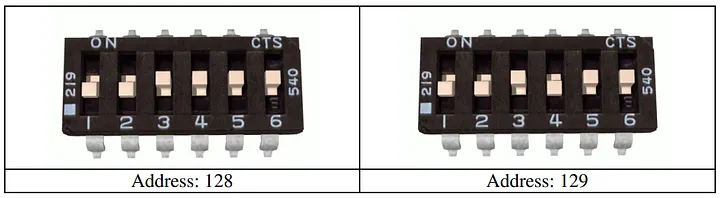
\includegraphics[width=0.75\linewidth]{figures/photos/sabertooth_dip_switch_article.png}
\caption{Sabertooth address setup reference from the original RUDRA material.  Verify against the current Dimension Engineering user guide before changing switch positions.}
\end{figure}

\section{Command mapping}
The RUDRAv4 bridge maps joystick or \topic{/cmd_vel} intent into left and right commands.  At the low level, each command is saturated to the Sabertooth signed command limit:
\begin{equation}
D_L=\mathrm{sat}_{[-127,127]}(k_v v - k_\omega \omega), \qquad
D_R=\mathrm{sat}_{[-127,127]}(k_v v + k_\omega \omega).
\end{equation}

For manual PS2 operation, the current behavior preserves the older RUDRA mixing convention:
\begin{equation}
\mathrm{left}=\mathrm{throttle}-\mathrm{steering}, \qquad
\mathrm{right}=\mathrm{throttle}+\mathrm{steering}.
\end{equation}

In closed-loop operation, those commands become wheel-speed targets; encoder feedback is used to reduce the difference between requested and measured wheel velocity.

\section{Regeneration and battery safety}
A regenerative driver can push energy back toward the battery during deceleration or when the robot is driven by external forces.  This is useful but it makes power wiring important.  The motor battery must remain connected when the Sabertooths are powered, and the emergency stop should remove motive power in a controlled manner.  Do not test motors with a weak supply, floating battery connection, or undersized bench supply that cannot tolerate regen.

\section{Motor bring-up procedure}
\begin{enumerate}
  \item Disconnect or lift all wheels.
  \item Confirm motor battery polarity and Sabertooth power wiring.
  \item Confirm each Sabertooth address with a small command.
  \item Send zero command and verify all motors stop.
  \item Send low positive left and right commands independently.
  \item Fix sign errors in firmware mapping, not by swapping random wires after the robot is assembled.
  \item Confirm the command timeout stops all motors when the NUC serial bridge is killed.
  \item Only then place the robot on the floor at low speed.
\end{enumerate}

\begin{safetybox}{Single owner of the Teensy serial port}
Never run \pkg{ps2_uno_to_teensy} and \pkg{cmd_vel_to_teensy} at the same time.  Both attempt to own the Teensy USB serial device, and both can generate motor commands.  Pick one drive bridge per test.
\end{safetybox}


\chapter{Teensy 4.1, Arduino Uno, and PS2 Controller Layer}
\label{chap:teensy-uno-ps2}

RUDRAv4 deliberately splits microcontroller responsibilities.  The Arduino Uno reads the wireless PS2 controller and sends compact joystick packets to the NUC.  The Teensy 4.1 receives final motor commands from the NUC, commands both Sabertooth drivers, and returns acknowledgements, IMU data, and wheel odometry.  This split is not accidental; it keeps manual input, ROS supervision, and motor safety understandable.

\section{Teensy 4.1 as the base controller}
The Teensy 4.1 is fast enough to own the base hardware loop while still exposing a simple USB serial interface to Linux.  It has independent hardware serial ports, which is why RUDRA can use USB serial for NUC communication and \cmd{Serial1} for the Sabertooth packet-serial bus.

\begin{figure}[h]
\centering
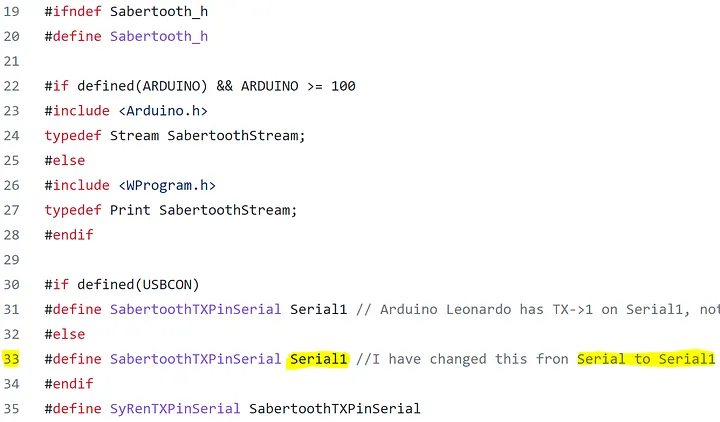
\includegraphics[width=0.72\linewidth]{figures/photos/sabertooth_serial1_article.png}
\caption{Firmware note from legacy assets: the Teensy uses a hardware serial port for Sabertooth communication while USB serial remains available to the NUC.}
\end{figure}

Current firmware files in the RUDRAv4 workspace are:

\begin{lstlisting}[caption={RUDRAv4 firmware locations.}]
src/rudra_base_bridge/firmware/uno_ps2_plain_serial/uno_ps2_plain_serial.ino
src/rudra_base_bridge/firmware/teensy_sabertooth_serial_controller/teensy_sabertooth_serial_controller.ino
src/rudra_base_bridge/firmware/teensy_sabertooth_imu_odom_controller/teensy_sabertooth_imu_odom_controller.ino
\end{lstlisting}

\section{Arduino Uno as the PS2 input controller}
The Uno keeps the PS2 receiver isolated from the main motor controller.  The current Uno packet is:

\begin{lstlisting}[caption={Uno to NUC joystick packet.}]
J,select,ry,rx,ly,lx,guard
\end{lstlisting}

The known PS2 receiver pin configuration from the RUDRA material is:

\begin{lstlisting}[language=C++,caption={PS2X receiver pin mapping.}]
ps2x.config_gamepad(9, 7, 6, 8, true, true);
// clock=9, command=7, attention=6, data=8
\end{lstlisting}

\begin{figure}[h]
\centering
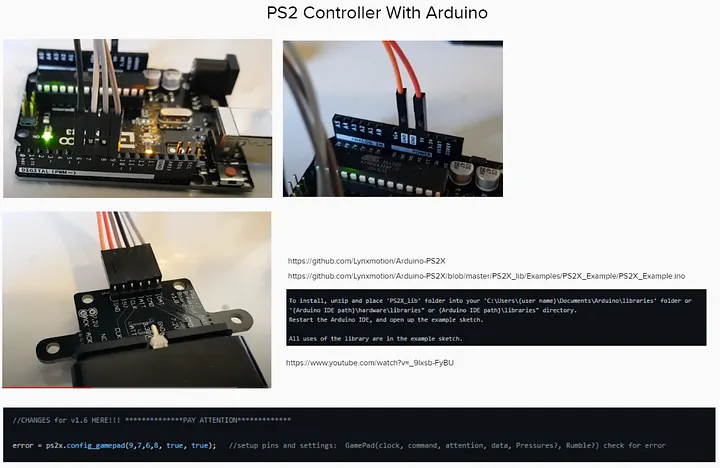
\includegraphics[width=0.92\linewidth]{figures/photos/ps2_controller_arduino_photo.png}
\caption{PS2 controller with Arduino reference image from the RUDRA article assets.}
\end{figure}

\section{Guard latch semantics}
The seventh Uno field, \cmd{guard}, is a latched obstacle-guard command.  Pressing \cmd{START} toggles the latch in the Uno firmware.  The ROS bridge follows that state and publishes \topic{/rudra/obstacle_guard}.  This means obstacle-guard enablement is observable in ROS rather than hidden in a controller sketch.

\section{Teensy command and acknowledgement contract}
The current manual drive path sends this line from the NUC to the Teensy:

\begin{lstlisting}[caption={NUC to Teensy drive packet.}]
D,left,right,enable
\end{lstlisting}

The Teensy replies with an acknowledgement line such as:

\begin{lstlisting}[caption={Teensy acknowledgement packet.}]
ACK,left,right,enable
\end{lstlisting}

For localization firmware, the Teensy also emits telemetry:

\begin{lstlisting}[caption={Teensy telemetry packet types.}]
IMU,ax,ay,az,gx,gy,gz
ODOM,x,y,theta,linear_x,angular_z,left_vel,right_vel
\end{lstlisting}

These packets are not a debug print afterthought.  They are the firmware-to-ROS contract.  Changing a field order in firmware must be matched by a change in the ROS parser and documented in the serial-protocol chapter.

\section{Firmware timing}
The Teensy should perform three timing-sensitive tasks even if ROS is temporarily delayed:

\begin{enumerate}
  \item Maintain a command watchdog.  If no valid command arrives within the timeout, write zero motor commands.
  \item Keep motor-output updates deterministic.  The Sabertooth bus is slow compared with internal MCU execution, so command scheduling must be simple.
  \item Keep encoder and IMU acquisition independent of Linux scheduling jitter.
\end{enumerate}

\begin{figure}[htbp]
\centering
\resizebox{0.90\linewidth}{!}{%
\begin{tikzpicture}[node distance=10mm and 14mm, every node/.append style={font=\small}]
  \node[rudraHw,text width=22mm] (ps2) {PS2\\receiver};
  \node[rudraBlock,text width=28mm,right=of ps2] (uno) {Arduino Uno\\\cmd{J,...}};
  \node[rudraBlock,text width=34mm,right=of uno] (nuc) {NUC ROS bridge\\topics and guard};
  \node[rudraBlock,text width=33mm,below=12mm of nuc] (teensy) {Teensy~4.1\\\cmd{D,...}, \cmd{ACK,...},\\IMU, ODOM};
  \node[rudraHw,text width=31mm,right=of teensy] (st) {Two Sabertooths};
  \draw[rudraArrow] (ps2) -- (uno);
  \draw[rudraArrow] (uno) -- node[above=0.5]{\scriptsize USB 115200} (nuc);
  \draw[rudraArrow] (nuc) -- node[left]{\scriptsize USB 115200} (teensy);
  \draw[rudraArrow] (teensy) -- node[above=0.75]{\scriptsize Serial1 9600} (st);
\end{tikzpicture}}
\caption{Microcontroller timing and ownership boundaries. The NUC supervises ROS-side behavior, while the Teensy remains the deterministic motor-control endpoint.}
\end{figure}

\section{Flashing workflow}
\begin{enumerate}
  \item Open the correct sketch in Arduino IDE or build it with Arduino CLI.
  \item Select the correct board: Uno for PS2 firmware, Teensy 4.1 for base firmware.
  \item Select the correct serial port.  Prefer \filep{/dev/serial/by-id} for runtime, but IDEs often display \filep{/dev/ttyACM*}.
  \item Upload the sketch.
  \item Close Serial Monitor before launching ROS.  Serial Monitor can hold the same port ROS needs.
  \item Run \cmd{bash scripts/list_serial.sh} again and update \filep{rudra_v4_hardware.yaml} if the by-id path changed.
\end{enumerate}

\section{Test ladder}
\begin{enumerate}
  \item Uno only: echo \topic{/rudra/ps2_raw}; sticks and SELECT should change.
  \item Teensy only: send neutral drive packets and expect \topic{/rudra/teensy_ack}.
  \item Teensy with wheels lifted: send low left/right commands.
  \item Full PS2 bridge with SELECT disabled: no wheel motion.
  \item Full PS2 bridge with SELECT enabled: low-speed manual motion.
  \item Kill the ROS launch while motors are spinning slowly: the Teensy watchdog must stop the motors.
\end{enumerate}


\chapter{Inertial Measurement Layer}
\label{chap:mpu6050}

RUDRAv4 uses an MPU6050-class six-axis inertial measurement unit.  The sensor provides three-axis acceleration and three-axis angular-rate measurements.  It does not provide a magnetometer.  Therefore, yaw will drift if it is only integrated from gyro rate.  The robot should use the IMU as one input to the localization stack, not as an absolute heading oracle.

\section{Sensor model}
The IMU output can be modeled as:
\begin{align}
\tilde{\boldsymbol{\omega}} &= \boldsymbol{\omega} + \boldsymbol{b}_{g} + \boldsymbol{n}_{g}, \\
\tilde{\boldsymbol{a}} &= \mathbf{R}^{T}(\boldsymbol{a}-\boldsymbol{g}) + \boldsymbol{b}_{a} + \boldsymbol{n}_{a},
\end{align}
where \(\tilde{\boldsymbol{\omega}}\) is the measured angular rate, \(\tilde{\boldsymbol{a}}\) is the measured acceleration, \(\boldsymbol{b}_{g}\) and \(\boldsymbol{b}_{a}\) are gyro and accelerometer biases, and \(\boldsymbol{n}_{g}\), \(\boldsymbol{n}_{a}\) are noise terms.

For a ground robot, the most important IMU signal is usually yaw rate about the vertical axis.  Roll and pitch are useful for sanity checking bumps and mounting errors, but RUDRA navigation depends mostly on planar motion.

\section{Firmware conversion}
The Teensy reads the MPU6050 over I2C.  Raw accelerometer and gyro counts must be converted exactly once.  Do not scale in firmware and then scale again on the NUC.

\begin{lstlisting}[caption={Current ROS topic contract for IMU telemetry.}]
Teensy packet: IMU,ax,ay,az,gx,gy,gz
ROS topic:     /rudra/imu/raw
ROS type:      sensor_msgs/msg/Imu
Frame:         imu_link
\end{lstlisting}

If the firmware sends acceleration in \(\mathrm{m/s^2}\) and gyro rate in \(\mathrm{rad/s}\), the ROS bridge should publish those values directly.  If the firmware sends raw counts, the ROS bridge must apply the conversion factors and document them.

\section{Frame convention}
The IMU frame must be fixed relative to \cmd{base_link}.  In the current localization launch, a static transform connects \cmd{base_link} to \cmd{imu_link}.  The physical orientation should be verified by moving the robot by hand and checking RViz or \topic{/rudra/imu/raw}:

\begin{enumerate}
  \item Push the robot forward gently.  The acceleration sign should match the expected \cmd{base_link} forward axis.
  \item Rotate the robot counterclockwise on the floor.  The yaw-rate sign should match ROS right-hand convention.
  \item Keep the robot still.  Gyro rates should settle near zero after bias, and acceleration magnitude should be near \SI{9.81}{m/s^2}.
\end{enumerate}

\section{Filtering and fusion}
Raw IMU data is noisy and biased.  RUDRAv4 uses the IMU with wheel odometry and \pkg{robot_localization}.  The conceptual filter state for a planar robot is:
\begin{equation}
\mathbf{x} = \begin{bmatrix} x & y & \theta & v_x & \omega_z \end{bmatrix}^{T}.
\end{equation}

Wheel odometry constrains planar position and velocity.  The IMU constrains angular velocity and, if orientation estimation is enabled, attitude.  The EKF prediction and update cycle is:
\begin{align}
\hat{\mathbf{x}}_{k|k-1} &= f(\hat{\mathbf{x}}_{k-1|k-1},\mathbf{u}_{k}) ,\\
\mathbf{P}_{k|k-1} &= \mathbf{F}_{k}\mathbf{P}_{k-1|k-1}\mathbf{F}_{k}^{T}+\mathbf{Q}_{k},\\
\mathbf{K}_{k} &= \mathbf{P}_{k|k-1}\mathbf{H}_{k}^{T}\left(\mathbf{H}_{k}\mathbf{P}_{k|k-1}\mathbf{H}_{k}^{T}+\mathbf{R}_{k}\right)^{-1},\\
\hat{\mathbf{x}}_{k|k} &= \hat{\mathbf{x}}_{k|k-1} + \mathbf{K}_{k}\left(\mathbf{z}_{k}-h(\hat{\mathbf{x}}_{k|k-1})\right).
\end{align}

\section{Practical calibration}
\begin{table}[h]
\centering
\caption{MPU6050 validation checks before trusting localization.}
\begin{tabularx}{\linewidth}{p{0.26\linewidth}Y}
\toprule
Check & What to do \\
\midrule
Static bias & Leave the robot still for 30 seconds, record gyro mean, and confirm yaw rate is near zero after correction. \\
Gravity magnitude & With the robot stationary, acceleration magnitude should be close to \SI{9.81}{m/s^2}. \\
Axis sign & Rotate the robot by hand and verify yaw-rate sign in ROS. \\
Vibration & Drive slowly on the floor and check if motor vibration creates spikes.  If yes, improve mounting and tune filter covariance. \\
Timestamp stability & IMU and odom messages should arrive with stable intervals.  Irregular bursts indicate serial parsing or firmware timing issues. \\
\bottomrule
\end{tabularx}
\end{table}

\section{Why the IMU does not replace wheel odometry}
An accelerometer integrated twice drifts quickly.  A gyro integrated once also drifts.  Encoders slip, but they are usually better for short-term planar translation.  The engineering solution is not choosing one sensor; it is fusing both sensors and monitoring when they disagree.


\chapter{LiDAR Scan and Obstacle Avoidance}
\label{chap:ydlidar-custom}

RUDRAv4 uses a YDLIDAR G2-class 360 degree laser scanner.  The current robot does not use the manufacturer's driver as a black box.  It keeps the YDLidar-SDK and \pkg{ydlidar_ros2_driver} in an external workspace and launches the driver through RUDRAv4-owned launch and parameter files.  That makes the LiDAR setup reproducible and keeps the robot's frame names, serial port, baud rate, and obstacle-guard behavior under version control.

\section{Why the driver is external}
The LiDAR driver depends on the vendor SDK.  Installing that SDK globally makes future rebuilds harder because the dependency is outside the workspace.  RUDRAv4 instead builds the SDK into \filep{/home/rudra/ros2_ws/install/YDLidar-SDK} and builds \pkg{ydlidar_ros2_driver} against that prefix.

\begin{lstlisting}[language=bash,caption={External LiDAR workspace overlay order.}]
source /opt/ros/lyrical/setup.bash
source /home/rudra/ros2_ws/install/setup.bash
source /home/rudra/Projects/RUDRAv4/install/setup.bash
\end{lstlisting}

\section{RUDRAv4 customization points}
The robot-owned files are:

\begin{lstlisting}[caption={LiDAR files owned by RUDRAv4.}]
src/rudra_base_bridge/launch/lidar.launch.py
src/rudra_base_bridge/config/ydlidar_g2b.yaml
scripts/run_lidar.sh
scripts/stop_lidar.sh
scripts/run_ps2_lidar_bridge.sh
scripts/run_ps2_lidar_localization.sh
\end{lstlisting}

The parameter file freezes the working robot settings:

\begin{lstlisting}[caption={Current RUDRAv4 YDLIDAR settings.}]
port: /dev/serial/by-id/usb-Silicon_Labs_CP2102_USB_to_UART_Bridge_Controller_0001-if00-port0
frame_id: laser
baudrate: 128000
lidar_type: 1
device_type: 0
sample_rate: 5
fixed_resolution: true
reversion: true
inverted: true
auto_reconnect: true
intensity: true
intensity_bit: 8
support_motor_dtr: false
range_min: 0.28
range_max: 16.0
frequency: 10.0
\end{lstlisting}

The exact baud rate and scan parameters should stay in the robot config rather than in a command typed by memory.

\section{LiDAR in the robot graph}
The LiDAR publishes \topic{/scan} in the \cmd{laser} frame.  The RUDRAv4 launch also publishes a static transform from \cmd{base_link} to \cmd{laser}.  This makes the scan visible in RViz and usable by the obstacle guard.

\begin{center}
\resizebox{0.98\linewidth}{!}{%
\begin{tikzpicture}[node distance=8mm and 11mm]
  \node[rudraHw] (lidar) {YDLIDAR G2B\\USB CP2102};
  \node[rudraBlock, right=of lidar] (driver) {\pkg{ydlidar_ros2_driver_node}};
  \node[rudraTopic, right=of driver] (scan) {\topic{/scan}\\\cmd{LaserScan}};
  \node[rudraBlock, below=of scan] (guard) {Obstacle guard\\front sector filter};
  \node[rudraTopic, left=of guard] (status) {\topic{/rudra/obstacle_guard}};
  \node[rudraTopic, right=of guard] (cmd) {filtered motor\\command};
  \draw[rudraArrow] (lidar) -- (driver);
  \draw[rudraArrow] (driver) -- (scan);
  \draw[rudraArrow] (scan) -- (guard);
  \draw[rudraArrow] (guard) -- (status);
  \draw[rudraArrow] (guard) -- (cmd);
\end{tikzpicture}}
\end{center}

\section{Known startup behavior}
The existing system manual captures practical LiDAR behavior that matters during launch: the first valid \topic{/scan} can take 10 to 15 seconds, startup checksum warnings can appear before scans begin, and the driver can print repeated fixed-point warnings while still publishing valid scans.  Therefore, the primary health signal is not a clean console; it is whether \topic{/scan} publishes with frame \cmd{laser}.

\begin{lstlisting}[language=bash,caption={LiDAR bring-up and validation.}]
cd /home/rudra/Projects/RUDRAv4
source /opt/ros/lyrical/setup.bash
source /home/rudra/ros2_ws/install/setup.bash
source install/setup.bash
bash scripts/run_lidar.sh /dev/serial/by-id/usb-Silicon_Labs_CP2102_USB_to_UART_Bridge_Controller_0001-if00-port0

# In another terminal
ros2 topic echo --once /scan
ros2 topic hz /scan
\end{lstlisting}

\section{Obstacle guard mathematics}
The guard examines a frontal angular sector and computes the minimum valid range in that sector.  If the scan angle for beam \(i\) is \(\alpha_i\), then the forward sector is:
\begin{equation}
\left|\alpha_i\right| \leq \frac{\alpha_{front}}{2}.
\end{equation}

Let \(r_{min}\) be the minimum finite range in that sector.  The command scale for forward motion is conceptually:
\begin{equation}
s(r_{min}) =
\begin{cases}
0, & r_{min} \leq r_{stop},\\
\dfrac{r_{min}-r_{stop}}{r_{slow}-r_{stop}}, & r_{stop}<r_{min}<r_{slow},\\
1, & r_{min}\geq r_{slow}.
\end{cases}
\end{equation}

Current RUDRAv4 defaults are \(\alpha_{front}=70^\circ\), \(r_{stop}=\SI{0.45}{m}\), and \(r_{slow}=\SI{1.00}{m}\).  Reverse and turn-in-place commands are allowed so the robot can back away from an obstacle.

\section{Debugging no scan}
\begin{enumerate}
  \item Run \cmd{bash scripts/list_serial.sh} and verify the CP2102 by-id path.
  \item Source the external LiDAR workspace before the RUDRAv4 workspace.
  \item Launch \cmd{lidar.launch.py} without any drive bridge.
  \item Wait at least 15 seconds before declaring failure.
  \item Echo \topic{/scan}; then check RViz with fixed frame \cmd{base_link} and LaserScan reliability set to Best Effort.
  \item If the LiDAR still spins after shutdown, remember that the motor is still powered by USB; cut USB power or unplug it.
\end{enumerate}


\chapter{RUDRAv4 Hardware}
\label{chap:body-batteries-bom}

This chapter documents the physical robot stack: chassis, drive motors, motor battery, NUC battery, wiring, and the visible bill of materials.  The hardware is the same RUDRA base used in the earlier article except the robot computer is now the Intel NUC, not the Jetson Nano, and the NUC is powered through the Mini-Box DCDC-USB.

\section{Robot body}
The robot body is the Lynxmotion A4WD1 aluminum 4WD rover platform.  It is a differential-drive platform: the two left wheels act as the left track, and the two right wheels act as the right track.  The base can drive forward, reverse, arc-turn, or spin in place by commanding different left and right wheel velocities.

\begin{figure}[h]
\centering
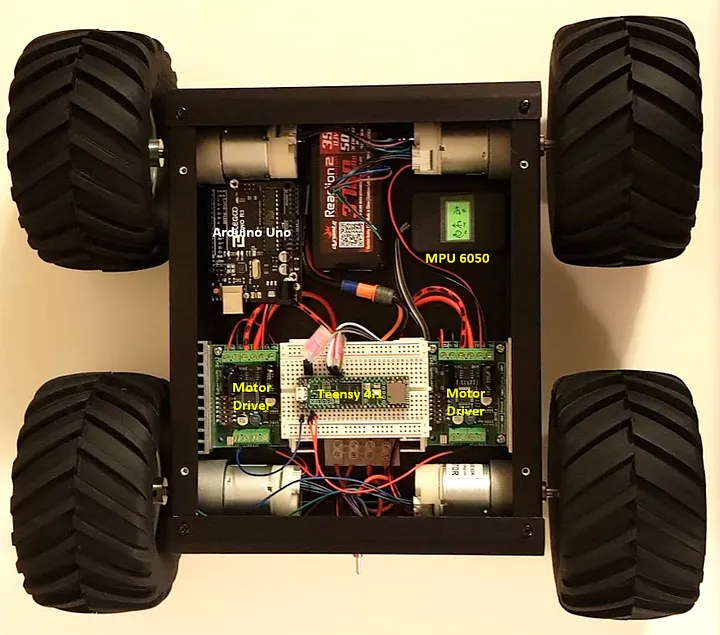
\includegraphics[width=0.88\linewidth]{figures/photos/rudra_chassis_top.png}
\caption{RUDRA chassis and deck layout reference from the engineering asset set.}
\end{figure}

For a 4WD skid-steer/differential rover, the ideal kinematic model is still the differential-drive model:
\begin{align}
v &= \frac{v_R+v_L}{2},\\
\omega &= \frac{v_R-v_L}{b},
\end{align}
where \(v\) is forward velocity, \(\omega\) is yaw rate, \(v_R\) and \(v_L\) are right and left side linear wheel velocities, and \(b\) is the wheelbase/track-width term used by the controller.  Real skid steer also includes scrub and slip, so odometry must be treated as a measured estimate, not ground truth.

\section{RUDRAv4 battery architecture}
RUDRAv4 uses two battery domains:

\begin{table}[h]
\centering
\caption{Battery domains used by RUDRAv4.}
\begin{tabularx}{\linewidth}{p{0.18\linewidth}p{0.27\linewidth}p{0.23\linewidth}Y}
\toprule
Domain & Pack & Nominal voltage & Purpose \\
\midrule
Motor power & Dynamite Reaction 2, 3S, \SI{11.1}{V}, 50C, \SI{41.07}{Wh} & \SI{11.1}{V} & Feeds Sabertooth motor drivers and drive motors. \\
NUC power & OVONIC, \SI{1550}{mAh}, 100C, 4S1P, \SI{14.8}{V}, \SI{22.94}{Wh} & \SI{14.8}{V} & Feeds Mini-Box DCDC-USB, which regulates to the NUC 19 V class input. \\
\bottomrule
\end{tabularx}
\end{table}

\begin{designbox}{Corrected OVONIC pack capacity}
The NUC battery is \SI{1550}{mAh}.  At \SI{14.8}{V} nominal, the stated pack energy is consistent: \(1.55\,\mathrm{Ah}\times14.8\,\mathrm{V}=\SI{22.94}{Wh}\).  Use the label value and measured runtime for operating decisions.
\end{designbox}

\section{Battery calculations}
For a LiPo pack:
\begin{equation}
E_{Wh}=V_{nominal} \times C_{Ah}.
\end{equation}

For the motor pack:
\begin{equation}
C_{Ah}=\frac{41.07}{11.1}=\SI{3.70}{Ah}.
\end{equation}

For the NUC pack as stated by capacity and nominal voltage:
\begin{equation}
E_{Wh}=14.8 \times 1.55=\SI{22.94}{Wh}.
\end{equation}

The approximate runtime is:
\begin{equation}
t_{hr}=\frac{E_{Wh}\eta}{P_{load}}.
\end{equation}

\begin{center}
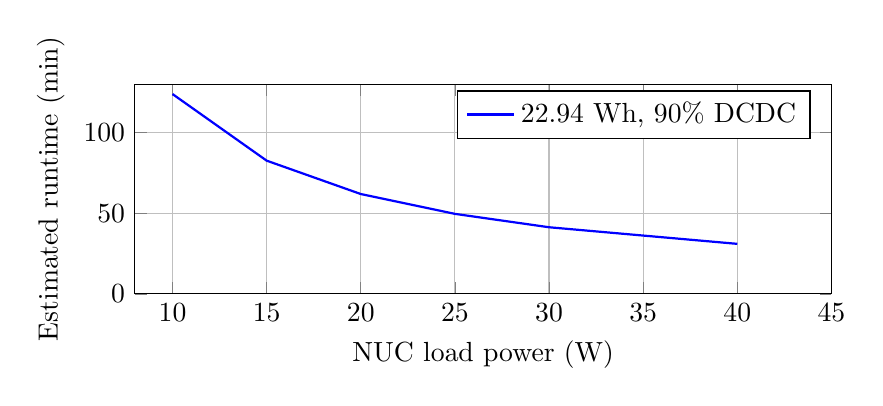
\begin{tikzpicture}
\begin{axis}[
  width=0.86\linewidth,
  height=0.35\linewidth,
  xlabel={NUC load power (W)},
  ylabel={Estimated runtime (min)},
  xmin=8,xmax=45,
  ymin=0,ymax=130,
  grid=both,
  legend pos=north east]
\addplot+[mark=none,thick] coordinates {(10,123.9) (15,82.6) (20,61.9) (25,49.6) (30,41.3) (40,31.0)};
\addlegendentry{22.94 Wh, 90\% DCDC}
\end{axis}
\end{tikzpicture}
\end{center}

The plot shows why the NUC battery should be monitored.  A small 4S pack can boot and run the NUC, but runtime depends strongly on CPU load, LiDAR/USB load, Wi-Fi, and DCDC efficiency.

\section{C-rating caution}
Theoretical discharge current from C-rating is:
\begin{equation}
I_{max,theory}=C_{rating} \times C_{Ah}.
\end{equation}

For the motor battery this gives \(50\times3.70=\SI{185}{A}\).  For the NUC battery using \SI{1.55}{Ah}, it gives \(100\times1.55=\SI{155}{A}\).  These values are marketing/pack capability indicators, not a reason to omit fuses, wire sizing, connector checks, or thermal checks.  The robot should be designed around measured current, connector limits, wiring gauge, and safe fuse ratings.

\section{Physical wiring and BOM reference}
The full wiring image from the RUDRA article remains valuable as the physical architecture reference.

\begin{figure}[h]
\centering
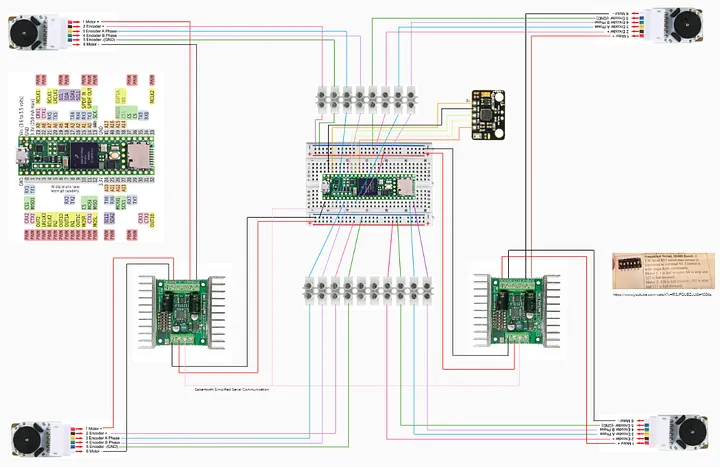
\includegraphics[width=0.96\linewidth]{figures/photos/rudra_wiring_detailed_full.png}
\caption{Detailed RUDRA base wiring reference: Teensy, Sabertooths, motors, IMU, encoder wiring, and power distribution.}
\end{figure}

The attached BOM screenshot is preserved below as a visual procurement reference.  It should not replace a version-controlled BOM file, but it is useful in the manual because it shows the real component stack used during the RUDRA build.

\begin{figure}[h]
\centering
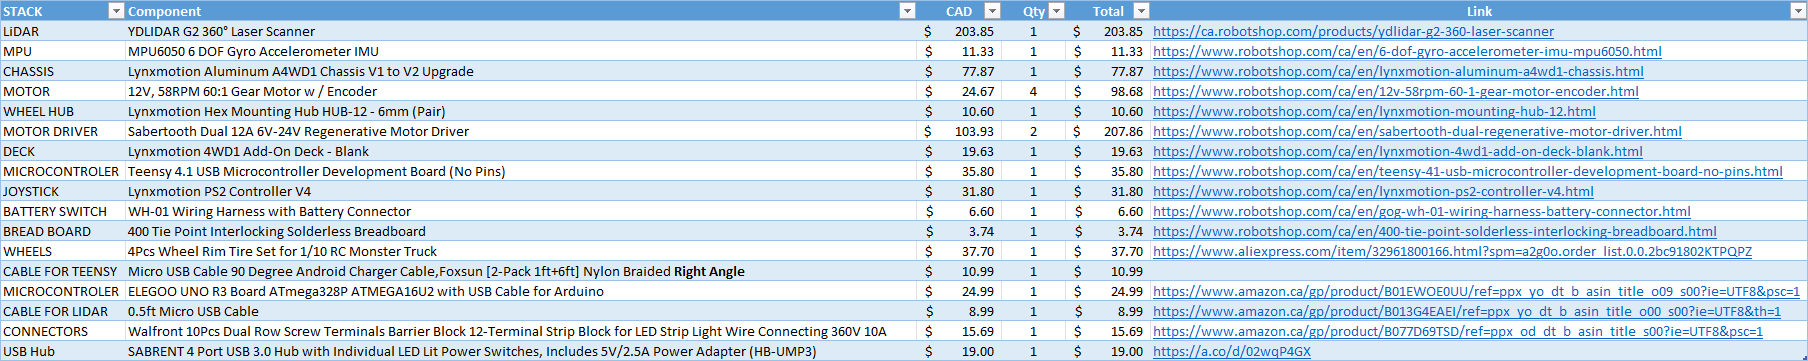
\includegraphics[width=0.96\linewidth]{figures/photos/rudra_bom_screenshot.png}
\caption{RUDRA hardware BOM screenshot supplied with this revision.  Keep the spreadsheet/source BOM under version control for exact part numbers, quantities, prices, and links.}
\end{figure}

\section{Mechanical integration notes}
\begin{itemize}
  \item Mount the NUC so the barrel connector and USB cables have strain relief.
  \item Keep the DCDC-USB and NUC power wiring away from the Sabertooth motor output wiring where practical.
  \item Route encoder and IMU signal wiring away from high-current motor leads.
  \item Secure LiPo packs mechanically; do not let them move during a sudden stop.
  \item Do not charge LiPo packs while installed inside a closed robot deck.
  \item Put an inline fuse or switch in the motor battery path and a separate accessible disconnect for the NUC rail.
\end{itemize}

\section{Verification before closing the deck}
\begin{enumerate}
  \item All grounds that must be common are common; power domains remain intentionally separated where required.
  \item Motor battery powers only the motor side.
  \item NUC battery powers the DCDC-USB input only.
  \item DCDC-USB output is verified before connecting to the NUC.
  \item USB cables are data-capable, not charge-only.
  \item \cmd{bash scripts/list_serial.sh} shows Uno, Teensy, and YDLIDAR adapter.
  \item \topic{/rudra/nuc_battery} publishes when the DCDC monitor is launched.
\end{enumerate}

\chapter{Engineering System Schematics}
\label{chap:engineering-schematics}

This chapter adds the high-level engineering interconnect sheets for the current RUDRAv4 hardware stack.  The intent is to provide a clean, reviewable system schematic that sits one level above the pictorial wiring image: it separates compute power, motor power, USB/data connections, packetized Sabertooth control, encoder feedback, and IMU wiring into two readable sheets.

\begin{designbox}{How to use these sheets}
Use these schematics as the engineering map for bring-up and troubleshooting.  Use Sheet 1 for power-domain and NUC-level wiring checks.  Use Sheet 2 for Teensy, Sabertooth, encoder, IMU, and PS2 controller pin-level checks.  The schematics intentionally avoid pictorial wire clutter and use named nets/off-page references so the drawing remains readable in print.
\end{designbox}

\begin{landscape}
\begin{figure}[p]
\centering
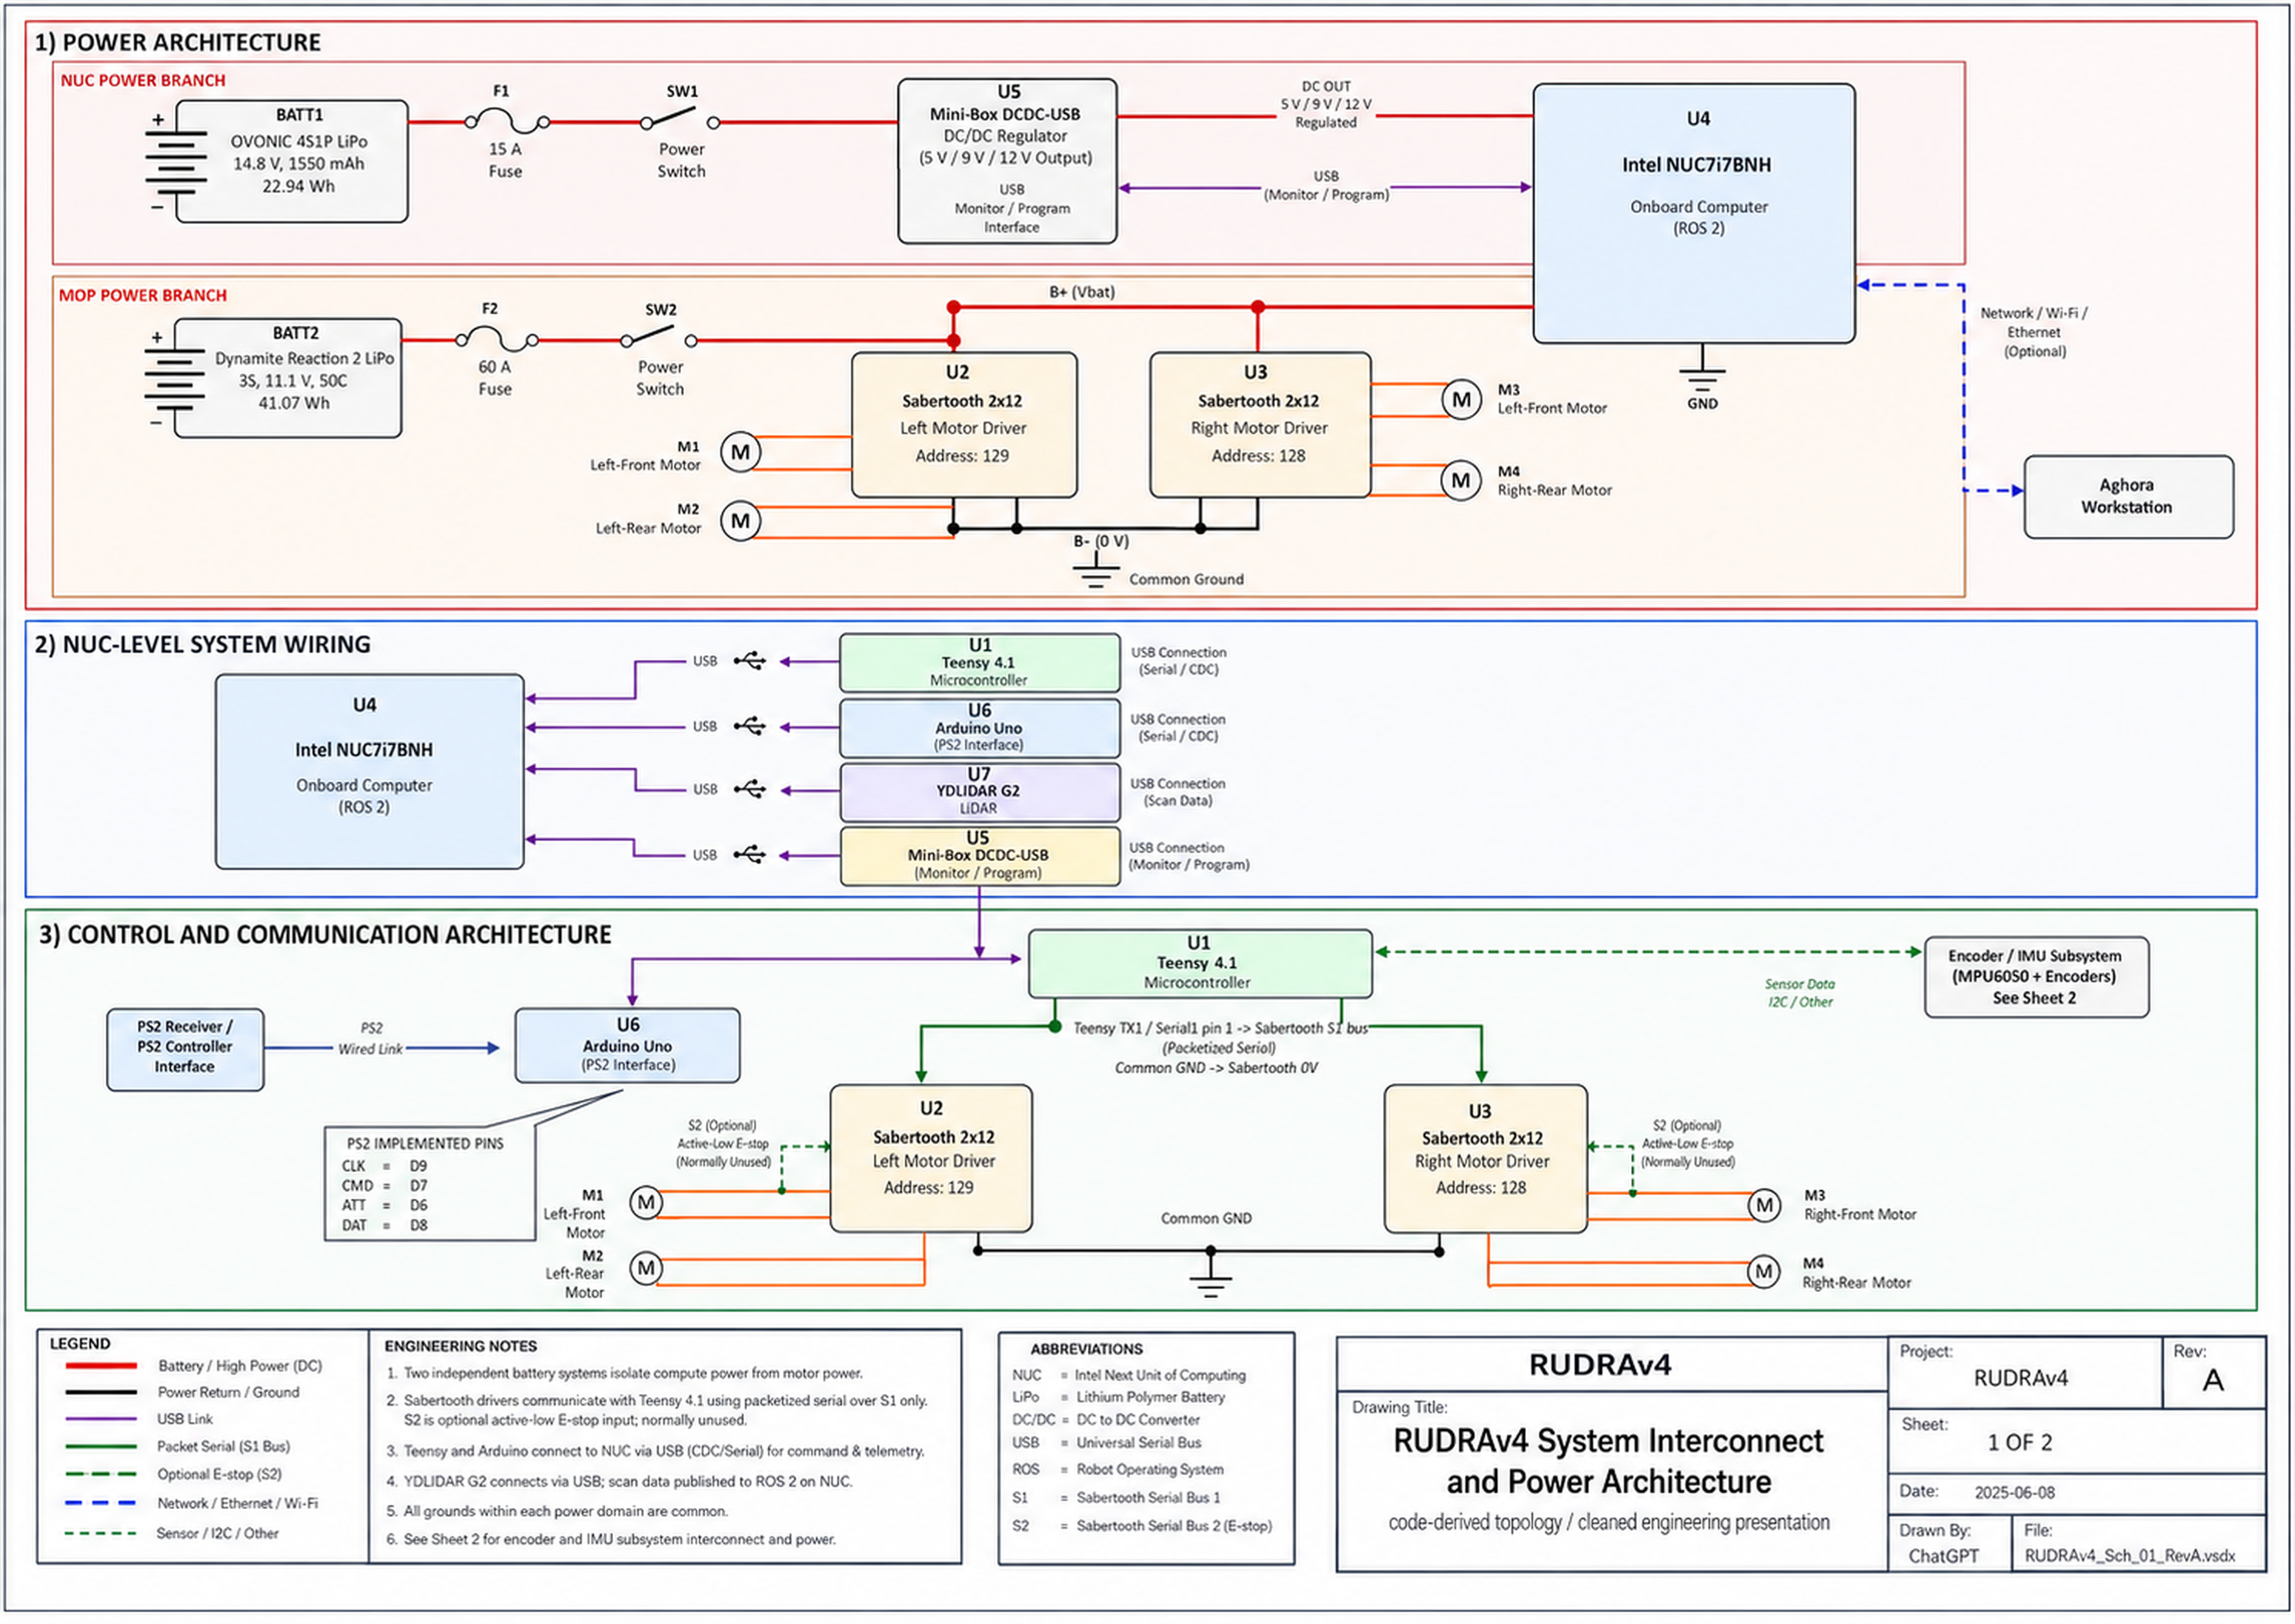
\includegraphics[width=0.96\linewidth,height=0.82\textheight,keepaspectratio]{figures/schematics/rudrav4_system_interconnect_schematic_highres.png}
\caption{RUDRAv4 Sheet 1 of 2: system interconnect and power architecture.  This sheet shows the NUC power branch through the Mini-Box DCDC-USB, the motor power branch through the Sabertooth drivers, the NUC USB wiring to Teensy/Uno/YDLIDAR/DCDC-USB, and the high-level control and communication architecture.}
\label{fig:rudra-sch-sheet1}
\end{figure}
\end{landscape}

\begin{landscape}
\begin{figure}[p]
\centering
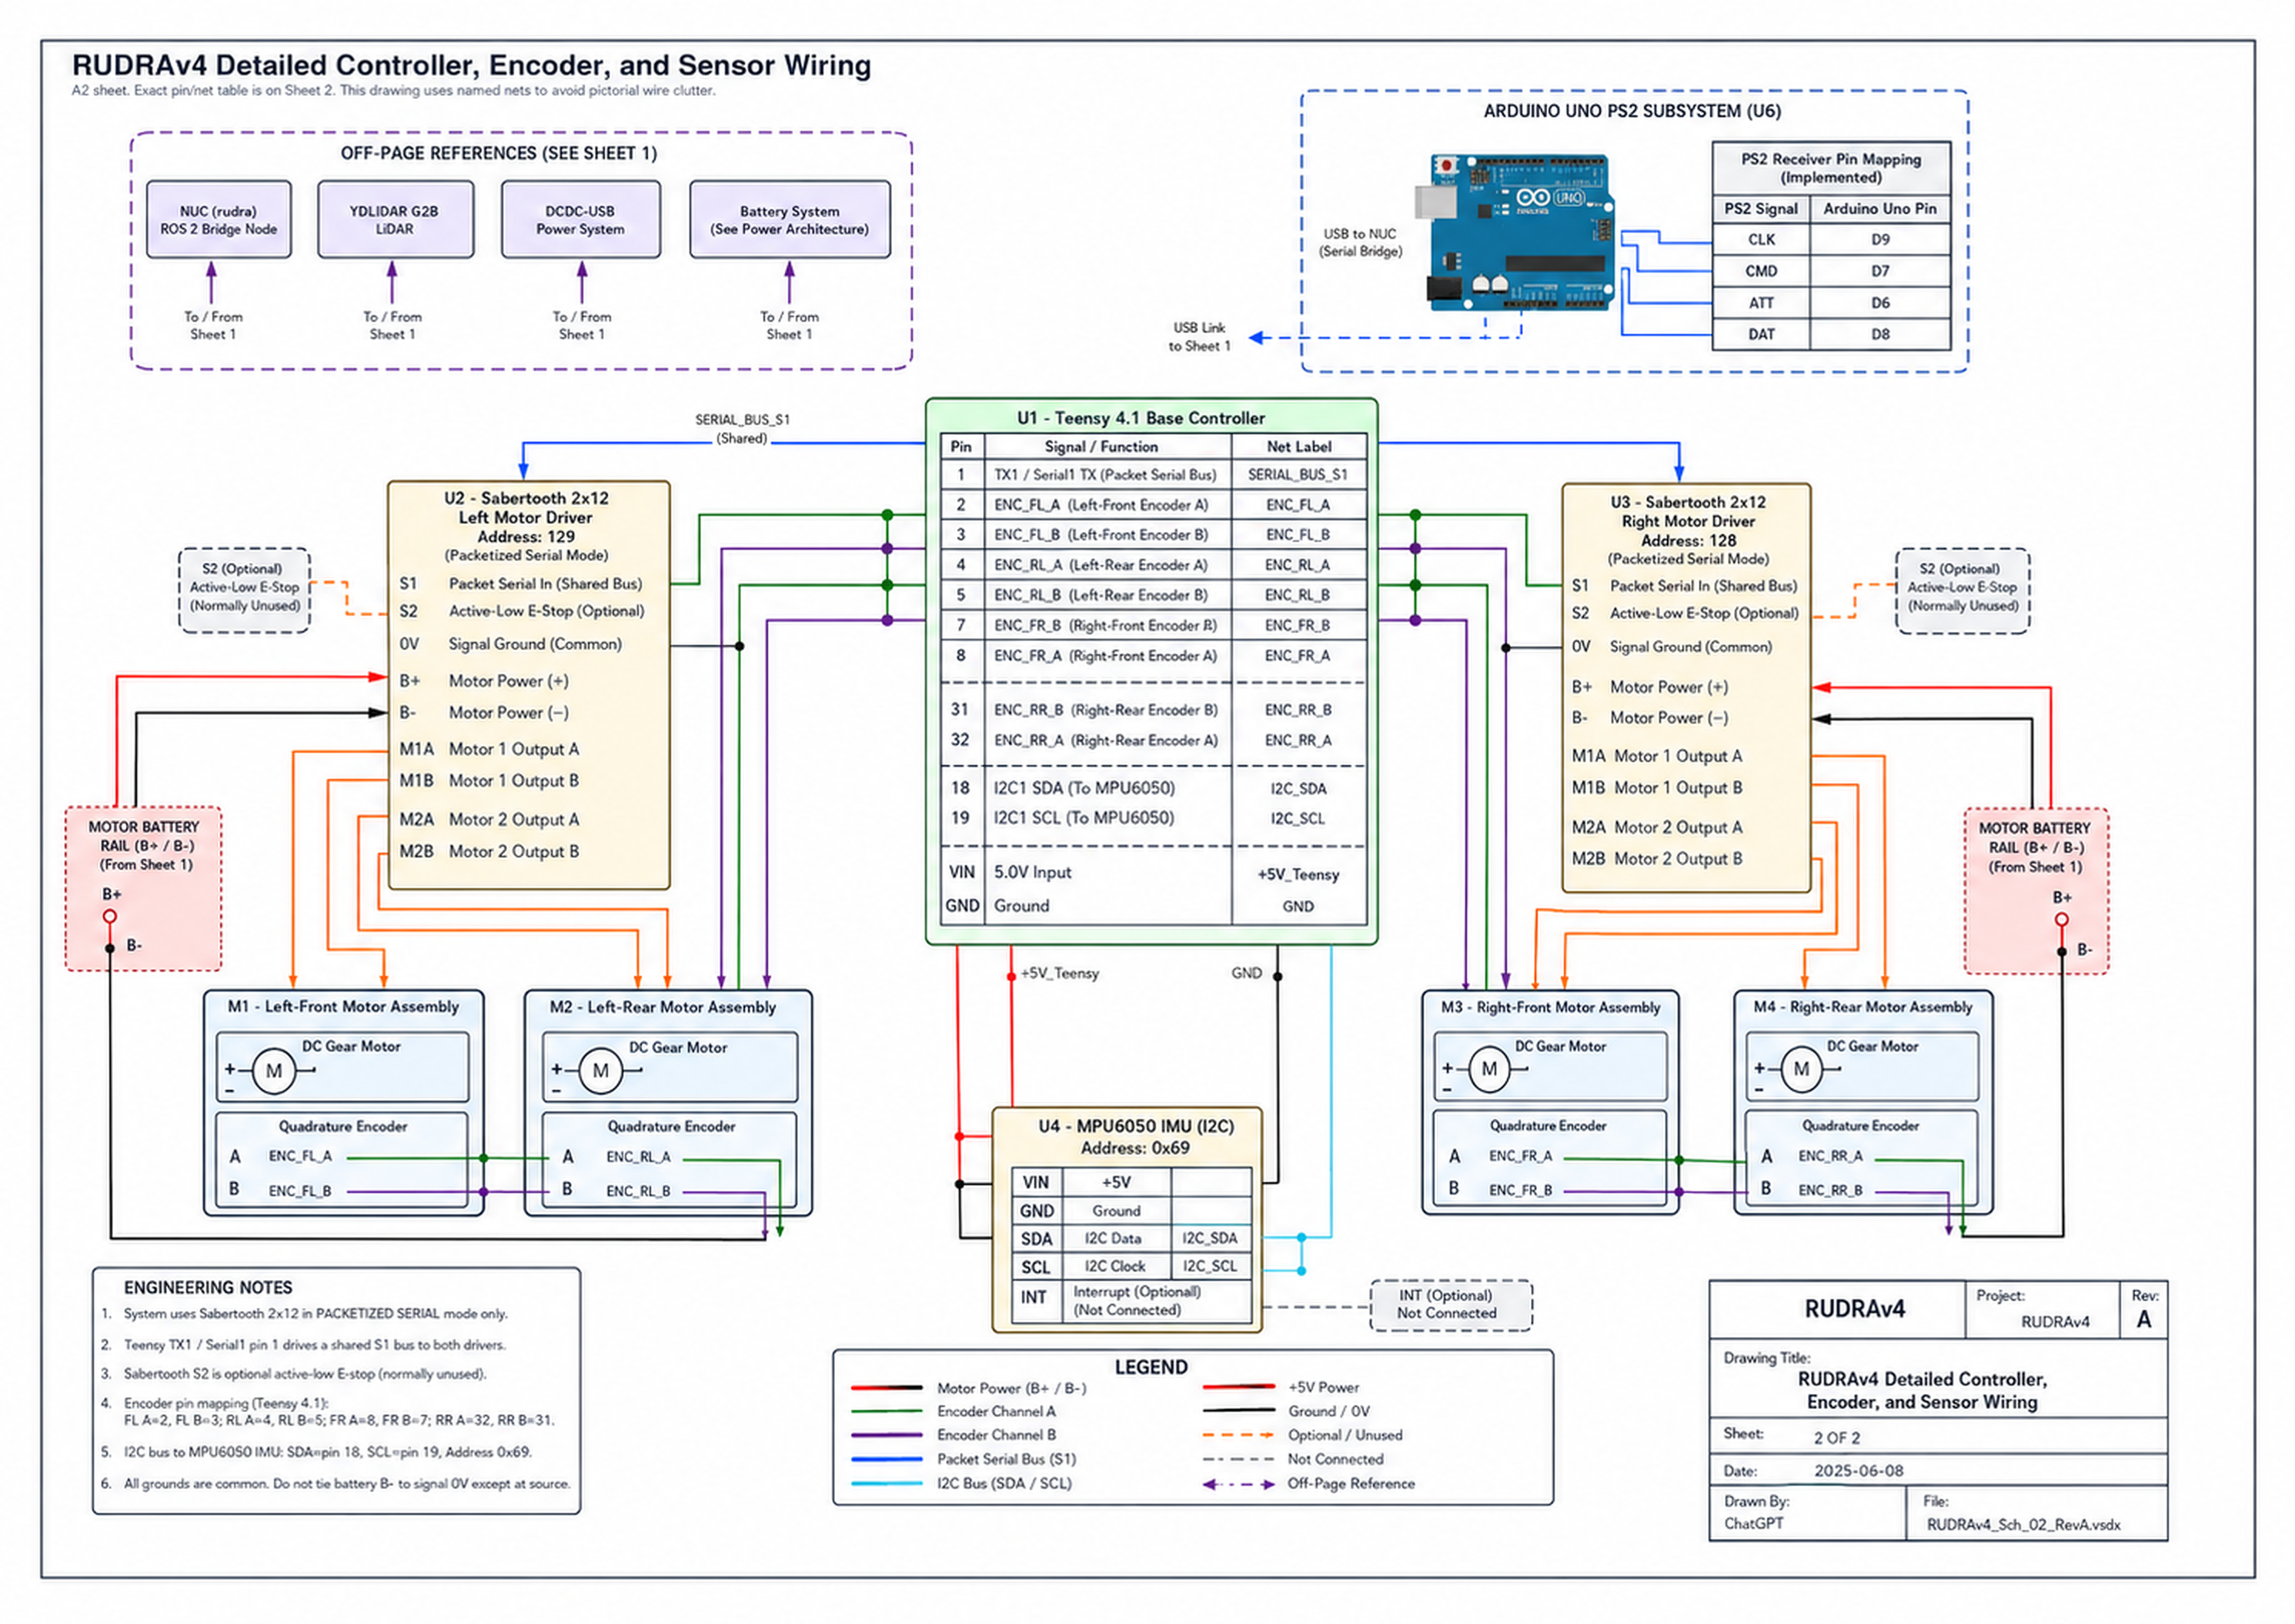
\includegraphics[width=0.96\linewidth,height=0.82\textheight,keepaspectratio]{figures/schematics/rudrav4_controller_wiring_schematic_highres.png}
\caption{RUDRAv4 Sheet 2 of 2: detailed controller, encoder, and sensor wiring.  This sheet documents the implemented Teensy pin mapping, shared packetized-serial Sabertooth S1 bus, optional S2 e-stop concept, motor/encoder wiring, MPU6050 I2C wiring, and Arduino Uno PS2 receiver pin mapping.}
\label{fig:rudra-sch-sheet2}
\end{figure}
\end{landscape}

\section{Schematic interpretation notes}

The two-sheet schematic set should be read with the firmware contracts in \cref{chap:teensy-uno-ps2,chap:sabertooth}.  The important implementation constraints are:

\begin{itemize}
  \item Sabertooth command is packetized serial, not PWM/DIR.
  \item Teensy \cmd{TX1}/\cmd{Serial1} drives the shared Sabertooth \cmd{S1} bus.
  \item Sabertooth \cmd{S2} is shown as optional active-low emergency stop and is not used as an RX channel.
  \item The NUC owns the ROS graph and connects by USB to the Teensy, Uno, YDLIDAR, and DCDC-USB monitor/programming interface.
  \item The NUC LiPo and motor LiPo are separate power branches; grounds are handled intentionally at the documented boundaries.
\end{itemize}

\chapter{Firmware Architecture}

\section{Why firmware is split}

RUDRAv4 has two microcontroller firmware roles. The Uno is a controller reader. The Teensy is a drive interface. This separation prevents PS2 controller library issues from interfering with Sabertooth packet serial timing, and it avoids forcing the Uno to handle tasks beyond its capacity.

\begin{figure}[htbp]
\centering
\resizebox{0.94\linewidth}{!}{\begin{tikzpicture}[node distance=9mm and 12mm, every node/.append style={font=\small}]
\node[rudraHw,text width=37mm] (uno) {Uno firmware\\\filep{uno_ps2_plain_serial.ino}};
\node[rudraBlock,text width=28mm,right=of uno] (nuc) {NUC ROS bridge};
\node[rudraHw,text width=32mm,right=of nuc] (teensy) {Teensy firmware\\drive + telemetry};
\node[rudraHw,text width=27mm,right=of teensy] (sabers) {Sabertooth\\drivers};
\draw[rudraArrow] (uno) -- node[above=0.75,align=center]{\scriptsize \cmd{J,select,ry,rx,ly,lx,guard}} (nuc);
\draw[rudraArrow] (nuc) -- node[above=0.75,align=center]{\scriptsize \cmd{D,left,right,enable}} (teensy);
\draw[rudraArrow] (teensy) -- node[above=0.75]{\scriptsize packet serial} (sabers);
\draw[rudraDashed] (teensy.south) to[bend right=-20] node[below,align=center]{\scriptsize \cmd{ACK}\\\cmd{IMU}\\\cmd{ODOM}} (nuc.south);
\end{tikzpicture}}
\caption{Firmware data contracts. The NUC is the translation layer between joystick packets, ROS topics, and drive packets.}
\end{figure}

\section{Uno PS2 firmware}

The Uno sketch is:

\begin{lstlisting}[language=bash]
src/rudra_base_bridge/firmware/uno_ps2_plain_serial/uno_ps2_plain_serial.ino
\end{lstlisting}

Its job is deliberately small:

\begin{itemize}
  \item configure the PS2 controller interface on pins CLK=9, CMD=7, ATT=6, DAT=8;
  \item poll the controller at roughly 20 Hz;
  \item latch manual mode on SELECT rising edge;
  \item latch obstacle guard enable on START rising edge;
  \item print one compact serial line per loop.
\end{itemize}

The emitted line is:

\begin{lstlisting}[language={}]
J,select,ry,rx,ly,lx,guard
\end{lstlisting}

The fields are raw and intentionally simple. The Uno does not know the robot kinematics. It does not know obstacle distance. It does not know Sabertooth addresses. It simply exposes operator intent to the NUC.

\section{Teensy base-drive firmware}

The plain drive firmware is:

\begin{lstlisting}[language=bash]
src/rudra_base_bridge/firmware/teensy_sabertooth_serial_controller/teensy_sabertooth_serial_controller.ino
\end{lstlisting}

It accepts:

\begin{lstlisting}[language={}]
D,left,right,enable
\end{lstlisting}

where \cmd{left} and \cmd{right} are clamped to \([-127,127]\) and \cmd{enable} is 0 or 1. If enabled, the target commands are ramped toward the requested values. If disabled or timed out, both targets go to zero.

The ramp is:

\begin{equation}
u_{k+1}=u_k+\mathrm{sat}(u_{target}-u_k,-s,s),
\end{equation}

where \(s\) is the ramp step. The current sketch uses \cmd{RAMP_STEP=6}, \cmd{CONTROL_PERIOD_MS=20}, and \cmd{COMMAND_TIMEOUT_MS=300}. Disabled ramp-down uses twice the step to stop faster.

\section{Teensy IMU and odometry firmware}

The telemetry-capable firmware is:

\begin{lstlisting}[language=bash]
src/rudra_base_bridge/firmware/teensy_sabertooth_imu_odom_controller/teensy_sabertooth_imu_odom_controller.ino
\end{lstlisting}

It preserves the same drive command input but adds:

\begin{lstlisting}[language={}]
IMU,ax,ay,az,gx,gy,gz
ODOM,x,y,theta,linear_x,angular_z,left_vel,right_vel
\end{lstlisting}

This is important. The telemetry firmware is backward-compatible with the ROS bridge because the NUC already drains Teensy serial lines and routes telemetry lines to \topic{/rudra/imu/raw} and \topic{/rudra/wheel_odom}. Non-telemetry lines remain available as \topic{/rudra/teensy_ack}.

\section{IMU scale and encoder scale}

The MPU6050 constants in the current firmware are:

\begin{align}
\mathrm{ACCEL\_SCALE} &= \frac{1}{16384},\\
\mathrm{GYRO\_SCALE} &= \frac{1}{131},\\
g &= 9.81\ \mathrm{m/s^2},\\
\mathrm{deg2rad} &= \frac{\pi}{180}.
\end{align}

The conversion is:

\begin{align}
a_x &= (\mathrm{raw}_x-b_x)\frac{1}{16384}g,\\
\omega_z &= (\mathrm{raw}_{gz}-b_{gz})\frac{1}{131}\frac{\pi}{180}.
\end{align}

Encoder speed follows \cref{eq:encoder-speed}. The telemetry firmware uses four encoder objects: two left and two right. The side speeds are averaged before odometry is integrated.

\section{Firmware validation checklist}

\begin{operatorbox}{Firmware checks before ROS driving}
\begin{enumerate}
  \item With motor power removed, open the Uno serial monitor and confirm \cmd{BOOT,PS2_ERROR,0} or investigate any nonzero PS2 error.
  \item Move sticks and verify \cmd{J,...} changes.
  \item Press SELECT and confirm the second field toggles 0/1.
  \item Press START and confirm the seventh field toggles 0/1.
  \item With Teensy connected and motor power removed, send \cmd{D,0,0,0} and confirm \cmd{ACK,0,0,0}.
  \item Send small commands such as \cmd{D,10,10,1} only with wheels lifted.
  \item Confirm timeout stops commands when the NUC stops sending.
\end{enumerate}
\end{operatorbox}

\section{When to reflash}

Reflash the Uno only when the controller packet is wrong, PS2 library behavior is wrong, or the START guard latch is missing. Reflash the Teensy when \cmd{D,...} is not accepted, \cmd{ACK,...} is missing, Sabertooth outputs are wrong, encoder telemetry is wrong, or IMU telemetry is required. Avoid reflashing both boards at once during troubleshooting. Change one boundary at a time.

\chapter{ROS Workspace Architecture}

\section{Repository layout}

The robot repository is the workspace at:

\begin{lstlisting}[language=bash]
/home/rudra/Projects/RUDRAv4
\end{lstlisting}

The primary package is:

\begin{lstlisting}[language=bash]
src/rudra_base_bridge
\end{lstlisting}

The package is Python-based, but it carries firmware sketches, YAML configuration, RViz files, and launch files. This is acceptable for a robot-development workspace because the package is the unit of bringup, not merely the unit of Python code. The normal operator launch is \filep{rudra_full.launch.py}; lower-level launch files and shell wrappers remain available for commissioning individual subsystems.

\section{Node inventory}

\begin{longtable}{p{0.25\linewidth}p{0.25\linewidth}p{0.40\linewidth}}
\toprule
Executable & Source file & Purpose\\
\midrule
\pkg{ps2_uno_to_teensy} & \filep{ps2_uno_to_teensy.py} & Reads \cmd{J,...} from Uno, applies joystick mixing and obstacle guard, writes \cmd{D,...} to Teensy, publishes observability topics.\\
\pkg{cmd_vel_to_teensy} & \filep{cmd_vel_to_teensy.py} & Converts ROS \topic{/cmd_vel} into left/right Sabertooth commands and writes them to Teensy.\\
\pkg{dcdc_usb_monitor} & \filep{dcdc_usb_monitor.py} & Parses \cmd{dcdc-usb -a} output and publishes NUC battery state and diagnostics.\\
\pkg{odom_tf_broadcaster} & \filep{odom_tf_broadcaster.py} & Broadcasts \cmd{odom -> base_link} from odometry messages when localization is active.\\
\pkg{serial_port_list} & \filep{serial_port_list.py} & Helper to list serial ports.\\
\bottomrule
\end{longtable}

\section{Helper modules}

Three helper modules are central to maintainability:

\begin{description}
\item[\pkg{serial_utils.py}] Provides \pkg{LineSerial}, a reconnecting line-oriented wrapper around pyserial, plus clamp, map, and deadband helpers.
\item[\pkg{obstacle_guard.py}] Encapsulates LiDAR scan filtering and command scaling. Both bridge nodes use the same guard behavior.
\item[\pkg{teensy_telemetry.py}] Parses optional \cmd{IMU,...} and \cmd{ODOM,...} lines and publishes ROS messages.
\end{description}

This modularity matters because the two drive bridges should not maintain two independent obstacle-guard implementations or two independent telemetry parsers.

\section{Launch file inventory}

\begin{longtable}{p{0.31\linewidth}p{0.59\linewidth}}
\toprule
Launch file & Role\\
\midrule
\filep{rudra_full.launch.py} & Main operator launch. Starts PS2 manual bridge, Teensy serial owner, LiDAR, obstacle guard, localization, voice, and optional Ollama, RViz, and DCDC monitoring.\\
\filep{rudra_ps2.launch.py} & Starts manual PS2 bridge only.\\
\filep{rudra_ps2_lidar.launch.py} & Starts PS2 bridge, YDLIDAR driver, and static \cmd{base_link -> laser} transform.\\
\filep{rudra_ps2_lidar_localization.launch.py} & Includes PS2+LiDAR launch, includes localization launch, and can optionally start DCDC monitor.\\
\filep{cmd_vel_to_teensy.launch.py} & Starts the autonomous or teleop \topic{/cmd_vel} bridge.\\
\filep{lidar.launch.py} & Starts only the YDLIDAR driver and static LiDAR transform.\\
\filep{lidar_view.launch.py} & Starts RViz view for scan and obstacle marker. It does not start a driver.\\
\filep{localization.launch.py} & Starts EKF, odom TF broadcaster, and \cmd{base_link -> imu_link} static transform.\\
\filep{localization_view.launch.py} & Starts RViz view for odometry, fused odometry, scan, and transforms.\\
\filep{dcdc_usb_monitor.launch.py} & Starts NUC power monitor only.\\
\filep{rudra_voice.launch.py} & Starts the voice node and command guard. The full launch includes this when \cmd{enable_voice:=true}.\\
\bottomrule
\end{longtable}

\begin{figure}[htbp]
\centering
\resizebox{0.98\linewidth}{!}{\begin{tikzpicture}[node distance=7mm]
\node[rudraBlock] (full) {\filep{rudra_full.launch.py}};
\node[rudraBlock,below left=of full] (base) {\filep{rudra_ps2_lidar_localization.launch.py}};
\node[rudraBlock,below right=of full] (voice) {\filep{rudra_voice.launch.py}};
\node[rudraBlock,below=of full] (helpers) {optional\\Ollama, RViz, DCDC};
\node[rudraBlock,below left=of base] (ps2lidar) {\filep{rudra_ps2_lidar.launch.py}};
\node[rudraBlock,below right=of base] (loc) {\filep{localization.launch.py}};
\node[rudraTopic,below left=of ps2lidar] (ps2) {\pkg{ps2_uno_to_teensy}};
\node[rudraTopic,below=of ps2lidar] (lidar) {\pkg{ydlidar_ros2_driver_node}};
\node[rudraTopic,below right=of ps2lidar] (tf1) {static TF\\\cmd{base_link -> laser}};
\node[rudraTopic,below left=of loc] (ekf) {\pkg{ekf_filter_node}};
\node[rudraTopic,below=of loc] (tf2) {\pkg{odom_tf_broadcaster}};
\node[rudraTopic,below right=of loc] (imu_tf) {static TF\\\cmd{base_link -> imu_link}};
\draw[rudraArrow] (full) -- (base);
\draw[rudraArrow] (full) -- (voice);
\draw[rudraDashed] (full) -- (helpers);
\draw[rudraArrow] (base) -- (ps2lidar);
\draw[rudraArrow] (base) -- (loc);
\draw[rudraArrow] (ps2lidar) -- (ps2);
\draw[rudraArrow] (ps2lidar) -- (lidar);
\draw[rudraArrow] (ps2lidar) -- (tf1);
\draw[rudraArrow] (loc) -- (ekf);
\draw[rudraArrow] (loc) -- (tf2);
\draw[rudraArrow] (loc) -- (imu_tf);
\end{tikzpicture}}
\caption{Launch dependency tree for the full robot bringup.}
\end{figure}

\section{Configuration files}

The three YAML files form the runtime contract:

\begin{description}
\item[\filep{rudra_v4_hardware.yaml}] Base bridge parameters: ports, baud, timeouts, joystick mapping, maximum speeds, obstacle guard parameters, telemetry topics, and DCDC thresholds.
\item[\filep{ydlidar_g2b.yaml}] YDLIDAR parameters: port, frame, baudrate, sample rate, scan range, frequency, intensity mode, and inversion/reversion flags.
\item[\filep{localization_ekf.yaml}] EKF parameters: two-dimensional mode, frames, wheel odom input, IMU input, selected measurement variables, queue sizes, and timeouts.
\end{description}

\section{Build model}

The repository build uses \cmd{colcon}. The minimal robot package build is:

\begin{lstlisting}[language=bash]
cd /home/rudra/Projects/RUDRAv4
bash scripts/install_deps.sh
source /opt/ros/lyrical/setup.bash
colcon build --packages-select rudra_base_bridge
source install/setup.bash
\end{lstlisting}

The checked-in \filep{scripts/build_ws.sh} wraps this idea. The build output goes into \filep{install/}. The runtime source order must still be respected in every terminal that launches robot nodes.

\section{Why wrapper scripts still exist}

The full launch is the normal operator path. Wrapper scripts are retained for subsystem commissioning because they set domain variables, source overlays, select known-good config files, and reduce typing mistakes while testing one boundary at a time. For example:

\begin{lstlisting}[language=bash]
bash scripts/run_ps2_lidar_localization.sh
\end{lstlisting}

is useful when proving the PS2, LiDAR, and EKF stack before adding voice or optional helpers. Once commissioning passes, return to \filep{rudra_full.launch.py} for normal operation.

\chapter{Serial Protocols and Safety State Machines}

\section{Why plain serial}

RUDRAv4 uses plain, line-oriented serial at the microcontroller boundary. This is simpler than embedding ROS inside microcontrollers and is easier to test with a serial monitor. Every protocol line is human-readable, newline-terminated, and short.

\section{Uno to NUC protocol}

The Uno emits:

\begin{lstlisting}[language={}]
J,select,ry,rx,ly,lx,guard
\end{lstlisting}

\begin{longtable}{p{0.16\linewidth}p{0.18\linewidth}p{0.56\linewidth}}
\toprule
Field & Type/range & Meaning\\
\midrule
\cmd{J} & literal & Packet type: joystick.\\
\cmd{select} & 0 or 1 & Latched manual-enable mode toggled by SELECT.\\
\cmd{ry} & 0--255-ish raw & Right stick Y raw value. Used only for optional guard chord logic if enabled.\\
\cmd{rx} & 0--255-ish raw & Right stick X raw value. Used for steering.\\
\cmd{ly} & 0--255-ish raw & Left stick Y raw value. Used for throttle.\\
\cmd{lx} & 0--255-ish raw & Left stick X raw value. Published but not presently used for driving.\\
\cmd{guard} & 0 or 1 & Latched obstacle guard enable toggled by START.\\
\bottomrule
\end{longtable}

The bridge accepts both the new seven-field packet and the older six-field form. If the guard field is absent, the bridge cannot update guard state from the controller latch.

\section{NUC to Teensy protocol}

The NUC emits:

\begin{lstlisting}[language={}]
D,left,right,enable
\end{lstlisting}

\begin{longtable}{p{0.16\linewidth}p{0.18\linewidth}p{0.56\linewidth}}
\toprule
Field & Type/range & Meaning\\
\midrule
\cmd{D} & literal & Packet type: drive command.\\
\cmd{left} & -127 to 127 & Left-side Sabertooth command after joystick mixing or \topic{/cmd_vel} conversion and obstacle filtering.\\
\cmd{right} & -127 to 127 & Right-side Sabertooth command.\\
\cmd{enable} & 0 or 1 & If 0, Teensy forces both sides to zero.\\
\bottomrule
\end{longtable}

The Teensy replies:

\begin{lstlisting}[language={}]
ACK,left,right,enable
ERR,bad_format
ERR,line_too_long
BOOT,RUDRA_TEENSY_SABERTOOTH_READY
BOOT,RUDRA_TEENSY_IMU_ODOM_READY
\end{lstlisting}

\section{Telemetry protocol}

The telemetry-capable Teensy firmware adds:

\begin{lstlisting}[language={}]
IMU,ax,ay,az,gx,gy,gz
ODOM,x,y,theta,linear_x,angular_z,left_vel,right_vel
\end{lstlisting}

The NUC parser treats these lines as telemetry and does not publish them as acknowledgements. All other Teensy lines go to \topic{/rudra/teensy_ack}. This allows the operator to see both control acknowledgement and richer telemetry without changing the base protocol.

\section{Timing and timeout}

The relevant timing constants are:

\begin{center}
\begin{tabular}{lcc}
\toprule
Loop & Period/timeout & Location\\
\midrule
Uno joystick print loop & 50 ms & Uno firmware\\
ROS bridge timer & 20 ms & Python node parameter\\
Teensy control loop & 20 ms & Teensy firmware\\
Teensy telemetry loop & 50 ms & telemetry firmware\\
Command timeout & 300 ms & ROS bridge and Teensy firmware\\
\bottomrule
\end{tabular}
\end{center}

The timeout design is layered. If the Uno disappears, the ROS bridge sends stop. If the NUC disappears, the Teensy times out and stops. If \topic{/cmd_vel} disappears, the \topic{/cmd_vel} bridge sends stop. No single software loop should be the only stop mechanism.

\begin{figure}[htbp]
\centering
\resizebox{0.98\linewidth}{!}{\begin{tikzpicture}[x=1cm,y=1cm]
\draw[->,thick] (0,0) -- (12,0) node[right]{time};
\foreach \x/\lab in {0/0,2/100ms,4/200ms,6/300ms,8/400ms,10/500ms} {
  \draw (\x,0.1) -- (\x,-0.1) node[below]{\lab};
}
\draw[rudraTeal,thick] (0,1.2) -- (5.8,1.2);
\draw[rudraAmber,thick] (5.8,1.2) -- (10.5,1.2);
\node[left] at (0,1.2) {commands};
\node[above] at (2.8,1.2) {valid \cmd{D,...}};
\node[above] at (8.2,1.2) {no update};
\draw[dashed] (6,0) -- (6,1.6);
\node[above] at (6,1.6) {timeout boundary};
\draw[rudraArrow] (6,0.65) -- (7.8,0.65) node[right]{Teensy forces target to zero};
\end{tikzpicture}}
\caption{Command timeout model. If fresh commands stop for more than about 300 ms, the Teensy disables drive.}
\end{figure}

\section{State machines}

The joystick bridge has a simple safety state machine:

\begin{enumerate}
  \item \textbf{No Uno / bad line}: send stop.
  \item \textbf{Valid packet but manual disabled}: send stop if configured.
  \item \textbf{Valid packet and enabled}: mix throttle/steering, apply obstacle guard, send drive.
  \item \textbf{Packet timeout}: send stop and publish zero \topic{/cmd_vel} preview.
\end{enumerate}

The Teensy state machine is even smaller:

\begin{enumerate}
  \item Parse latest \cmd{D,...} line.
  \item Clamp and store targets if enabled, otherwise zero targets.
  \item If command timeout expires, zero targets.
  \item Ramp actual commands toward targets.
  \item Write packet serial outputs to both Sabertooths.
\end{enumerate}

This split keeps high-level decisions on the NUC while ensuring the motor interface still has a local timeout if the NUC or USB link fails.

\chapter{Manual Control Bridge}

\section{Purpose of \pkg{ps2_uno_to_teensy}}

The manual bridge is the normal operator-control path. It connects the PS2 controller chain to the Teensy drive chain and publishes enough ROS topics to make that connection visible.

\begin{figure}[htbp]
\centering
\resizebox{0.94\linewidth}{!}{\begin{tikzpicture}[node distance=9mm and 8mm, every node/.append style={font=\small}]
\node[rudraHw,text width=24mm] (uno) {Uno serial\\\cmd{J,...}};
\node[rudraBlock,text width=27mm,right=of uno] (parse) {Parse packet\\\pkg{Ps2Packet}};
\node[rudraBlock,text width=26mm,right=of parse] (mix) {Axis scale\\deadband\\tank mix};
\node[rudraBlock,text width=27mm,right=of mix] (guard) {LiDAR guard\\forward filter};
\node[rudraHw,text width=24mm,right=of guard] (teensy) {Teensy serial\\\cmd{D,...}};
\node[rudraTopic,text width=28mm,below=of parse] (raw) {\topic{/rudra/ps2_raw}};
\node[rudraTopic,text width=28mm,below=of mix] (cmdv) {\topic{/cmd_vel} preview};
\node[rudraTopic,text width=33mm,below=of guard] (stat) {\topic{/rudra/obstacle_guard}};
\node[rudraTopic,text width=34mm,below=of teensy] (drive) {\topic{/rudra/drive_cmd}\\\topic{/rudra/teensy_ack}};
\draw[rudraArrow] (uno) -- (parse);
\draw[rudraArrow] (parse) -- (mix);
\draw[rudraArrow] (mix) -- (guard);
\draw[rudraArrow] (guard) -- (teensy);
\draw[rudraDashed] (parse) -- (raw);
\draw[rudraDashed] (mix) -- (cmdv);
\draw[rudraDashed] (guard) -- (stat);
\draw[rudraDashed] (teensy) -- (drive);
\end{tikzpicture}}
\caption{Manual bridge processing pipeline, redrawn with wider nodes and clearer spacing for print readability.}
\end{figure}

\section{Axis mapping}

The PS2 library returns raw analog values centered around 127. The bridge maps a raw axis value \(a\) into a signed command using:

\begin{align}
a_c &= a - a_0,\\
a_s &= \mathrm{round}\left(\frac{a_c}{a_{range}}u_{max}\right),\\
u &= \begin{cases}
0, & |a_s|\leq d,\\
\mathrm{sat}(a_s,-u_{max},u_{max}), & \text{otherwise},
\end{cases}
\end{align}

where \(a_0=127\), \(a_{range}=127\), \(u_{max}=127\), and the current deadband is \(d=15\).

The bridge inverts Ly and Rx so the physical controller direction matches the robot convention used during earlier RUDRA development.

\section{Manual mixing}

After scaling, the bridge computes:

\begin{align}
throttle &= f(Ly),\\
steering &= f(Rx),\\
left &= \mathrm{sat}(throttle-steering,-127,127),\\
right &= \mathrm{sat}(throttle+steering,-127,127).
\end{align}

SELECT toggles manual enable in the Uno firmware. When manual enable is false, the bridge sends \cmd{D,0,0,0} if \param{send_stop_when_disabled} is true.

\section{Obstacle-guard latch}

START toggles the guard latch in the Uno firmware. The seventh field of the joystick packet carries that latched state. The bridge compares the packet latch to the internal guard state and calls \cmd{set_enabled()} when they differ. This makes obstacle guarding an operator-visible mode rather than a hidden parameter.

\begin{safetybox}{Guard latch is not a safety-rated stop}
The LiDAR guard is a development safety layer for forward motion. It is not a certified safety system. It cannot see every obstacle, it depends on a valid \topic{/scan}, and it can be intentionally disabled. Keep physical control of motor power during tests.
\end{safetybox}

\section{Published topics}

\begin{longtable}{p{0.25\linewidth}p{0.18\linewidth}p{0.47\linewidth}}
\toprule
Topic & Type & Meaning\\
\midrule
\topic{/rudra/ps2_raw} & \cmd{String} & Raw joystick line from Uno.\\
\topic{/rudra/drive_cmd} & \cmd{String} & Final \cmd{D,left,right,enable} sent to Teensy.\\
\topic{/rudra/teensy_ack} & \cmd{String} & Non-telemetry response lines from Teensy.\\
\topic{/cmd_vel} & \cmd{Twist} & Preview of the manual command as a ROS velocity command.\\
\topic{/rudra/obstacle_guard} & \cmd{String} & Guard state, closest distance, and forward scale.\\
\topic{/rudra/imu_raw} & \cmd{Imu} & Optional telemetry parsed from Teensy.\\
\topic{/rudra/wheel_odom} & \cmd{Odometry} & Optional telemetry parsed from Teensy.\\
\bottomrule
\end{longtable}

\section{Launch}

Manual PS2-only bringup:

\begin{lstlisting}[language=bash]
cd /home/rudra/Projects/RUDRAv4
source /opt/ros/lyrical/setup.bash
source install/setup.bash
bash scripts/run_ps2_bridge.sh
\end{lstlisting}

Manual PS2 with LiDAR obstacle guard:

\begin{lstlisting}[language=bash]
cd /home/rudra/Projects/RUDRAv4
source /opt/ros/lyrical/setup.bash
source /home/rudra/ros2_ws/install/setup.bash
source install/setup.bash
bash scripts/run_ps2_lidar_bridge.sh \
  /dev/serial/by-id/usb-Silicon_Labs_CP2102_USB_to_UART_Bridge_Controller_0001-if00-port0
\end{lstlisting}

Manual PS2 with LiDAR, odometry, IMU, EKF, and optional power monitor:

\begin{lstlisting}[language=bash]
bash scripts/run_ps2_lidar_localization.sh
# or enable the DCDC monitor explicitly:
ros2 launch rudra_base_bridge rudra_ps2_lidar_localization.launch.py \
  enable_dcdc_monitor:=true
\end{lstlisting}

\section{Operator sequence}

\begin{enumerate}
  \item Confirm the robot is stable, wheels are lifted for first test, and motor power is controlled.
  \item Start the selected manual bridge launch.
  \item Echo \topic{/rudra/ps2_raw}. Move sticks and press SELECT/START to verify packet changes.
  \item Press SELECT once to enable manual mode.
  \item Use small stick deflections first. Watch \topic{/rudra/drive_cmd} and \topic{/rudra/teensy_ack}.
  \item If LiDAR is active, place an object inside the front cone and verify \topic{/rudra/obstacle_guard} changes before driving on the floor.
\end{enumerate}

\chapter{LiDAR and Obstacle Guard}

\section{YDLIDAR role}

The YDLIDAR is a USB serial sensor. Its ROS 2 driver publishes \topic{/scan} as \cmd{sensor_msgs/msg/LaserScan}. The scan is used by RViz, the obstacle guard, and future SLAM/navigation layers. The LiDAR is not wired into the Sabertooth chain; it influences motion only through the ROS bridge.

The current known-good LiDAR configuration is in:

\begin{lstlisting}[language=bash]
src/rudra_base_bridge/config/ydlidar_g2b.yaml
\end{lstlisting}

Important parameters include:

\begin{center}
\small
\begin{tabularx}{\linewidth}{p{0.22\linewidth}Y}
\toprule
Parameter & Value\\
\midrule
\param{port} & \filep{/dev/serial/by-id/usb-Silicon_Labs_CP2102_USB_to_UART_Bridge_Controller_0001-if00-port0}\\
\param{baudrate} & 128000\\
\param{frame_id} & \cmd{laser}\\
\param{sample_rate} & 5\\
\param{frequency} & 10.0\\
\param{range_min} & 0.28 m\\
\param{range_max} & 16.0 m\\
\param{intensity} & true\\
\bottomrule
\end{tabularx}
\end{center}

\section{LaserScan geometry}

A LaserScan message contains an array of ranges. Each index maps to an angle:

\begin{equation}
\theta_i=\theta_{min}+i\Delta\theta.
\end{equation}

Each valid point can be converted into LiDAR-frame Cartesian coordinates:

\begin{align}
x_i &= r_i\cos\theta_i,\\
y_i &= r_i\sin\theta_i.
\end{align}

The RUDRA obstacle guard does not build a map. It computes only the closest valid range inside a front cone.

\begin{figure}[htbp]
\centering
\resizebox{0.98\linewidth}{!}{\begin{tikzpicture}[scale=2.1]
\draw[->,thick] (0,0) -- (2.2,0) node[right]{front x};
\draw[->,thick] (0,-1.2) -- (0,1.2) node[above]{y};
\draw[rudraTeal,thick] (0,0) -- ({2*cos(35)},{2*sin(35)});
\draw[rudraTeal,thick] (0,0) -- ({2*cos(-35)},{2*sin(-35)});
\draw[rudraTealSoft,fill=rudraTealSoft,opacity=0.55] (0,0) -- ({2*cos(35)},{2*sin(35)}) arc (35:-35:2) -- cycle;
\draw[rudraAmber,thick,dashed] (0,0) circle (0.45);
\draw[rudraTeal,thick,dashed] (0,0) circle (1.0);
\node at (1.15,0.62) {front cone};
\node[rudraAmber] at (0.62,-0.18) {stop};
\node[rudraTeal] at (1.26,-0.18) {slow};
\fill[rudraAmber] (0.55,0.2) circle (0.04) node[above right]{closest obstacle};
\end{tikzpicture}}
\caption{Obstacle guard geometry. Only finite scan points inside the configured front cone are considered.}
\end{figure}

\section{Guard scale law}

The current guard parameters are:

\begin{align}
\phi_{front} &= 70^\circ,\\
d_{stop} &= 0.45\ \text{m},\\
d_{slow} &= 1.00\ \text{m},\\
t_{scan} &= 0.75\ \text{s}.
\end{align}

Let \(d\) be the closest valid front-cone obstacle distance. The forward scale is:

\begin{equation}
s(d)=
\begin{cases}
1, & \text{guard disabled},\\
1, & \text{no fresh scan},\\
1, & d \ge d_{slow},\\
0, & d \le d_{stop},\\
\dfrac{d-d_{stop}}{d_{slow}-d_{stop}}, & d_{stop}<d<d_{slow}.
\end{cases}
\end{equation}

For positive forward commands, the filtered command is:

\begin{equation}
u_{forward,filtered}=s(d)u_{forward}.
\end{equation}

Reverse and turn-in-place remain available so the robot can back away from an obstacle.

\begin{figure}[htbp]
\centering
\resizebox{0.98\linewidth}{!}{\begin{tikzpicture}
\begin{axis}[width=0.82\linewidth,height=6cm,xlabel={closest front distance (m)},ylabel={forward scale},xmin=0,xmax=1.4,ymin=-0.05,ymax=1.05,grid=both]
\addplot[thick,rudraTeal,domain=0:0.45,samples=2]{0};
\addplot[thick,rudraTeal,domain=0.45:1.0,samples=50]{(x-0.45)/(1.0-0.45)};
\addplot[thick,rudraTeal,domain=1.0:1.4,samples=2]{1};
\addplot[thick,rudraAmber,dashed] coordinates {(0.45,-0.05) (0.45,1.05)};
\addplot[thick,black,dashed] coordinates {(1.0,-0.05) (1.0,1.05)};
\node at (axis cs:0.23,0.12) {blocked};
\node at (axis cs:0.72,0.55) {slowing};
\node at (axis cs:1.18,0.92) {clear};
\end{axis}
\end{tikzpicture}}
\caption{Forward-speed scaling used by the obstacle guard.}
\end{figure}

\section{Marker and status output}

The guard publishes:

\begin{itemize}
  \item \topic{/rudra/obstacle_guard}: string status containing reason, enabled flag, closest front distance, and forward scale.
  \item \topic{/rudra/obstacle_guard_marker}: RViz marker at the closest front obstacle point.
\end{itemize}

Marker colors are:

\begin{center}
\begin{tabular}{ll}
\toprule
Marker color & Meaning\\
\midrule
Green & clear\\
Orange & slowing\\
Red & blocked\\
Gray & disabled\\
Deleted/no marker & no closest front point or stale scan\\
\bottomrule
\end{tabular}
\end{center}

\section{LiDAR startup behavior}

The YDLIDAR driver may take 10--15 seconds before the first valid scan appears. Startup checksum warnings and repeated fixed-point warnings can occur while scans are still valid. The operational test is not a warning-free console; it is whether \topic{/scan} publishes with frame \cmd{laser} and the scan is visible in RViz.

\section{Launching LiDAR}

LiDAR only:

\begin{lstlisting}[language=bash]
cd /home/rudra/Projects/RUDRAv4
source /opt/ros/lyrical/setup.bash
source /home/rudra/ros2_ws/install/setup.bash
source install/setup.bash
bash scripts/run_lidar.sh \
  /dev/serial/by-id/usb-Silicon_Labs_CP2102_USB_to_UART_Bridge_Controller_0001-if00-port0
\end{lstlisting}

View from Aghora:

\begin{lstlisting}[language=bash]
source /opt/ros/lyrical/setup.bash
export ROS_DOMAIN_ID=42
export ROS_LOCALHOST_ONLY=0
cd /home/rudra/Projects/RUDRAv4
source install/setup.bash
ros2 launch rudra_base_bridge lidar_view.launch.py
\end{lstlisting}

The viewer launch starts RViz only. It does not start the LiDAR driver and does not start a drive bridge.

\chapter{Localization, Odometry, and TF}

\section{The frame problem}

A mobile robot must report not only sensor values but also where those values live. RUDRA uses a standard planar frame chain:

\begin{equation}
\cmd{odom} \rightarrow \cmd{base_link} \rightarrow \cmd{laser}
\end{equation}

and:

\begin{equation}
\cmd{base_link} \rightarrow \cmd{imu_link}.
\end{equation}

\cmd{base_link} is the robot body frame. \cmd{laser} is the LiDAR frame. \cmd{imu_link} is the IMU frame. \cmd{odom} is a locally continuous frame used for odometry. A future SLAM layer can add:

\begin{equation}
\cmd{map} \rightarrow \cmd{odom}.
\end{equation}

\begin{figure}[htbp]
\centering
\resizebox{0.98\linewidth}{!}{\begin{tikzpicture}[node distance=11mm]
\node[rudraTopic] (map) {\cmd{map}\\future SLAM};
\node[rudraTopic,right=of map] (odom) {\cmd{odom}};
\node[rudraTopic,right=of odom] (base) {\cmd{base_link}};
\node[rudraTopic,above right=of base] (laser) {\cmd{laser}};
\node[rudraTopic,below right=of base] (imu) {\cmd{imu_link}};
\draw[rudraDashed] (map) -- node[above=0.5]{SLAM} (odom);
\draw[rudraArrow] (odom) -- node[above=0.5]{dynamic} (base);
\draw[rudraArrow] (base) -- node[above,sloped]{static} (laser);
\draw[rudraArrow] (base) -- node[below,sloped]{static} (imu);
\end{tikzpicture}}
\caption{RUDRAv4 TF tree. The map frame is not required for base bringup; it is introduced when SLAM is stable.}
\end{figure}

\section{Telemetry sources}

The localization layer expects the Teensy telemetry firmware to publish:

\begin{lstlisting}[language={}]
IMU,ax,ay,az,gx,gy,gz
ODOM,x,y,theta,linear_x,angular_z,left_vel,right_vel
\end{lstlisting}

The ROS bridge converts these into:

\begin{itemize}
  \item \topic{/rudra/imu/raw} as \cmd{sensor_msgs/msg/Imu}
  \item \topic{/rudra/wheel_odom} as \cmd{nav_msgs/msg/Odometry}
\end{itemize}

The IMU message intentionally leaves orientation unset by setting \cmd{orientation_covariance[0] = -1.0}. That tells downstream consumers that orientation is not available from this message.

That convention is important. A ROS IMU message with an arbitrary quaternion can be worse than no orientation at all, because downstream filters may treat it as a real attitude measurement. RUDRAv4 publishes raw acceleration and angular velocity first, then lets the EKF choose only the measurement components that are trustworthy for the current robot.

\section{Wheel odometry from encoder telemetry}

Wheel odometry is the robot's short-term estimate based on wheel motion. It is locally smooth but can drift because of wheel slip, floor irregularity, unequal wheel radius, encoder count errors, and unmodeled skid-steer effects. The mathematical basis was introduced in \cref{eq:pose-derivative}. For implementation, the robot integrates:

\begin{align}
x_k &= x_{k-1} + v_k\Delta t\cos\theta_k,\\
y_k &= y_{k-1} + v_k\Delta t\sin\theta_k,\\
\theta_k &= \theta_{k-1} + \Omega_k\Delta t.
\end{align}

This produces the \topic{/rudra/wheel_odom} message.

\section{IMU telemetry}

The MPU6050 provides acceleration and gyro readings. Gyro yaw rate is useful for correcting short-term yaw motion, but integrating gyro alone drifts over time. Acceleration is noisy and includes gravity components. Therefore, raw IMU is useful but should not be trusted alone for global pose.

The Teensy estimates gyro and accelerometer biases during startup by averaging stationary samples. Bias removal improves short-term behavior, but it is not a complete inertial navigation solution. Gyro bias changes with temperature, vibration, mounting stress, and supply noise. The correct use of this sensor in RUDRAv4 is therefore incremental: use yaw rate to stabilize local odometry, not to claim global heading.

\section{EKF fusion}

The ROS-side EKF is configured in:

\begin{lstlisting}[language=bash]
src/rudra_base_bridge/config/localization_ekf.yaml
\end{lstlisting}

The current filter runs in two-dimensional mode and uses:

\begin{itemize}
  \item \topic{/rudra/wheel_odom} for x, y, yaw, forward velocity, and yaw rate components.
  \item \topic{/rudra/imu/raw} for yaw-rate component only.
\end{itemize}

A simplified EKF model can be written as:

\begin{align}
\mathbf{x}_k &= f(\mathbf{x}_{k-1},\mathbf{u}_{k-1}) + \mathbf{w}_k,\\
\mathbf{z}_k &= h(\mathbf{x}_k) + \mathbf{v}_k,
\end{align}

where \(\mathbf{x}\) is the state estimate, \(\mathbf{z}\) is the measurement vector, \(\mathbf{w}\) is process noise, and \(\mathbf{v}\) is measurement noise. RUDRA's practical EKF value is not mathematical complexity; it is the disciplined combination of wheel and IMU signals into one consistent odometry output.

\subsection{Covariance as trust}

In ROS localization, covariance is how the system communicates uncertainty. Small covariance tells the filter that a measurement is trusted. Large covariance tells the filter that the measurement is noisy. A missing or overconfident covariance can destabilize fusion even when the raw numbers look plausible.

RUDRAv4 starts with conservative fixed covariances in the bridge:

\begin{itemize}
  \item IMU orientation covariance begins with \(-1\), meaning orientation is intentionally absent.
  \item IMU angular velocity covariance is small enough to use yaw rate, but not zero.
  \item Wheel odometry pose and twist covariances are nonzero because encoder odometry drifts and slips.
\end{itemize}

These values are engineering starting points. Tune them from logs: if fused yaw follows wheel slip too aggressively, reduce trust in wheel yaw; if fused yaw follows gyro drift too aggressively, reduce trust in IMU yaw rate.

\subsection{Two-dimensional mode}

The robot is a ground rover. It does not need to estimate altitude, roll, pitch, or lateral velocity for the current base-localization problem. The EKF therefore runs in two-dimensional mode. This reduces state ambiguity and avoids letting weak measurements corrupt unused degrees of freedom.

\section{Why publish TF outside the EKF}

The current EKF config sets \param{publish_tf: false}. The separate \pkg{odom_tf_broadcaster} subscribes to \topic{/odometry/filtered} and broadcasts \cmd{odom -> base_link}. This separation makes TF behavior explicit and easier to debug during development.

\section{Launch}

Full manual, LiDAR, localization stack:

\begin{lstlisting}[language=bash]
cd /home/rudra/Projects/RUDRAv4
source /opt/ros/lyrical/setup.bash
source /home/rudra/ros2_ws/install/setup.bash
source install/setup.bash
bash scripts/run_ps2_lidar_localization.sh
\end{lstlisting}

RViz localization view:

\begin{lstlisting}[language=bash]
bash scripts/view_localization.sh
\end{lstlisting}

In the localization view, fixed frame should be \cmd{odom}. Confirm the following:

\begin{itemize}
  \item raw wheel odom: \topic{/rudra/wheel_odom}
  \item fused odom: \topic{/odometry/filtered}
  \item scan: \topic{/scan}
  \item TF tree: \cmd{odom -> base_link -> laser} and \cmd{base_link -> imu_link}
\end{itemize}

\begin{operatorbox}{Localization bringup rule}
Do not add SLAM until odom, scan, and TF are stable. SLAM debugging is almost impossible if the base odometry or frame tree is already wrong.
\end{operatorbox}

\chapter{Launching, Operating, and Monitoring RUDRA}

\section{Pre-launch checklist}

Before launching robot nodes:

\begin{enumerate}
  \item Confirm motor power can be disconnected immediately.
  \item Confirm the wheels are lifted for the first test after any change.
  \item Confirm the Uno, Teensy, LiDAR, and DCDC-USB appear under \filep{/dev/serial/by-id} or expected USB listings.
  \item Close Arduino Serial Monitor or any terminal that owns a serial port.
  \item Confirm both Rudra and Aghora use \cmd{ROS_DOMAIN_ID=42} and \cmd{ROS_LOCALHOST_ONLY=0}.
  \item Source overlays in order: base ROS, external LiDAR workspace, then RUDRAv4.
\end{enumerate}

\section{Mode selection}

\begin{longtable}{p{0.24\linewidth}p{0.34\linewidth}p{0.32\linewidth}}
\toprule
Mode & Use when & Command\\
\midrule
PS2 only & Basic manual drive without LiDAR driver & \cmd{bash scripts/run_ps2_bridge.sh}\\
PS2 + LiDAR & Manual driving with \topic{/scan} and obstacle guard & \cmd{bash scripts/run_ps2_lidar_bridge.sh}\\
PS2 + LiDAR + localization & Full development bringup with IMU/wheel odom and EKF & \cmd{bash scripts/run_ps2_lidar_localization.sh}\\
\topic{/cmd_vel} bridge & Keyboard teleop, Nav2, autonomy, or external command publisher & \cmd{bash scripts/run_cmd_vel_bridge.sh}\\
LiDAR only & Sensor and RViz debug without drive bridge & \cmd{bash scripts/run_lidar.sh}\\
DCDC monitor only & Power rail debug & \cmd{ros2 launch rudra_base_bridge dcdc_usb_monitor.launch.py}\\
\bottomrule
\end{longtable}

\begin{safetybox}{One Teensy owner only}
Do not run \pkg{ps2_uno_to_teensy} and \pkg{cmd_vel_to_teensy} at the same time. Both write to the same Teensy serial port.
\end{safetybox}

\section{Full bringup sequence}

On Rudra:

\begin{lstlisting}[language=bash]
cd /home/rudra/Projects/RUDRAv4
bash scripts/list_serial.sh
source /opt/ros/lyrical/setup.bash
source /home/rudra/ros2_ws/install/setup.bash
source install/setup.bash
bash scripts/run_ps2_lidar_localization.sh
\end{lstlisting}

On Aghora:

\begin{lstlisting}[language=bash]
source /opt/ros/lyrical/setup.bash
export ROS_DOMAIN_ID=42
export ROS_LOCALHOST_ONLY=0
cd /home/rudra/Projects/RUDRAv4
source install/setup.bash
ros2 launch rudra_base_bridge localization_view.launch.py
\end{lstlisting}

\section{Monitoring commands}

Use a separate terminal for monitors:

\begin{lstlisting}[language=bash]
ros2 node list
ros2 topic list
ros2 topic echo /rudra/ps2_raw
ros2 topic echo /rudra/drive_cmd
ros2 topic echo /rudra/teensy_ack
ros2 topic echo /rudra/obstacle_guard
ros2 topic echo --once /scan
ros2 topic echo --once /rudra/imu/raw
ros2 topic echo --once /rudra/wheel_odom
ros2 topic echo --once /odometry/filtered
ros2 topic echo /rudra/nuc_battery
ros2 topic echo /diagnostics
\end{lstlisting}

\section{What good looks like}

\begin{longtable}{p{0.33\linewidth}p{0.57\linewidth}}
\toprule
Observation & Interpretation\\
\midrule
\topic{/rudra/ps2_raw} changes when sticks move & Uno and PS2 controller are reaching ROS.\\
\topic{/rudra/drive_cmd} shows bounded \cmd{D,...} lines & Bridge is computing final motor packets.\\
\topic{/rudra/teensy_ack} echoes \cmd{ACK,...} & Teensy is receiving drive commands.\\
\topic{/scan} publishes with frame \cmd{laser} & YDLIDAR driver is healthy enough for RViz and guard.\\
\topic{/rudra/obstacle_guard} changes when an obstacle is placed ahead & Scan reaches guard and forward scale logic is active.\\
\topic{/rudra/imu_raw} and \topic{/rudra/wheel_odom} publish & Telemetry firmware and parser are active.\\
\topic{/odometry/filtered} publishes & EKF has inputs and is alive.\\
RViz displays scan and marker & DDS domain, TF, and display settings are correct.\\
\bottomrule
\end{longtable}

\section{Shutdown}

A conservative shutdown order is:

\begin{enumerate}
  \item Release sticks or stop the \topic{/cmd_vel} publisher.
  \item Stop the drive launch with Ctrl-C.
  \item Stop LiDAR if needed:
\begin{lstlisting}[language=bash]
bash scripts/stop_lidar.sh
\end{lstlisting}
  \item Remove Sabertooth motor power.
  \item Shut down the NUC cleanly:
\begin{lstlisting}[language=bash]
sudo shutdown now
\end{lstlisting}
\end{enumerate}

If the LiDAR still spins, it is still receiving USB power. Remove USB power physically.

\chapter{Testing and Commissioning}

\section{Commissioning philosophy}

Commission RUDRA by proving each boundary before proving the whole robot. A system launch that starts every node is not proof that the robot is safe. The correct sequence is serial identity, firmware packets, drive packets, LiDAR scan, obstacle guard, telemetry, localization, then integrated motion.

\section{Stage 0: static inspection}

\begin{enumerate}
  \item Inspect all power wiring before connecting batteries.
  \item Confirm NUC power rail output with a multimeter.
  \item Confirm Sabertooth battery wiring and polarity.
  \item Confirm Teensy TX1 to Sabertooth S1 shared packet serial connection.
  \item Confirm Uno PS2 receiver pins CLK=9, CMD=7, ATT=6, DAT=8.
  \item Confirm LiDAR USB adapter is connected and mechanically secure.
\end{enumerate}

\section{Stage 1: serial identity}

Run:

\begin{lstlisting}[language=bash]
cd /home/rudra/Projects/RUDRAv4
bash scripts/list_serial.sh
\end{lstlisting}

Expected devices are Arduino Uno, Teensy, and CP2102 LiDAR adapter. Edit \filep{src/rudra_base_bridge/config/rudra_v4_hardware.yaml} if the persistent paths differ.

\section{Stage 2: firmware packet tests}

With motor power removed:

\begin{itemize}
  \item Open Uno serial and verify \cmd{J,...} output.
  \item Toggle SELECT and START and verify the correct packet fields change.
  \item Open Teensy serial and send \cmd{D,0,0,0}; verify \cmd{ACK,0,0,0}.
  \item Send \cmd{D,10,10,1}; verify ACK, then stop.
\end{itemize}

Do not move to powered motor tests until serial behavior is boring.

\section{Stage 3: ROS bridge tests}

Run the PS2 bridge with wheels lifted:

\begin{lstlisting}[language=bash]
bash scripts/run_ps2_bridge.sh
\end{lstlisting}

In another terminal:

\begin{lstlisting}[language=bash]
ros2 topic echo /rudra/ps2_raw
ros2 topic echo /rudra/drive_cmd
ros2 topic echo /rudra/teensy_ack
\end{lstlisting}

Confirm that enabling manual mode through SELECT is required before nonzero drive commands are sent.

\section{Stage 4: motor direction test}

With the robot lifted and motor power connected, use very small commands. The expected behavior is:

\begin{center}
\begin{tabular}{ll}
\toprule
Command intent & Expected motion\\
\midrule
small forward throttle & all wheels drive forward\\
small reverse throttle & all wheels drive reverse\\
small left turn & right side faster than left side\\
small right turn & left side faster than right side\\
spin & left and right sides opposite signs\\
\bottomrule
\end{tabular}
\end{center}

If one motor is reversed, fix polarity or motor mapping before changing ROS signs. If an entire side is reversed, investigate the side mapping between Teensy, Sabertooth, and motor wiring.

\section{Stage 5: LiDAR and guard test}

Run:

\begin{lstlisting}[language=bash]
bash scripts/run_ps2_lidar_bridge.sh
\end{lstlisting}

After scans begin, echo:

\begin{lstlisting}[language=bash]
ros2 topic echo /rudra/obstacle_guard
\end{lstlisting}

Place an object in front of the robot. The state should move from clear to slowing and then blocked as the object moves inside the stop distance. Reverse and turning should remain available.

\section{Stage 6: telemetry and localization}

Flash the telemetry Teensy firmware, then run:

\begin{lstlisting}[language=bash]
bash scripts/run_ps2_lidar_localization.sh
\end{lstlisting}

Confirm:

\begin{lstlisting}[language=bash]
ros2 topic echo --once /rudra/imu/raw
ros2 topic echo --once /rudra/wheel_odom
ros2 topic echo --once /odometry/filtered
\end{lstlisting}

Move the robot slowly and verify that odometry direction and yaw sign match physical motion. If forward motion decreases x, or left rotation decreases yaw when the frame convention expects the opposite, fix signs before attempting SLAM.

\section{Stage 7: power monitor test}

Run:

\begin{lstlisting}[language=bash]
dcdc-usb -a
ros2 launch rudra_base_bridge dcdc_usb_monitor.launch.py
ros2 topic echo /rudra/nuc_battery
ros2 topic echo /diagnostics
\end{lstlisting}

Compare reported input and output voltage to a multimeter. Validate thresholds before enabling shutdown.

\section{Stage 8: integrated full launch}

After the subsystem stages pass, use the canonical full launch with wheels lifted:

\begin{lstlisting}[language=bash]
cd /home/rudra/Projects/RUDRAv4
source /opt/ros/lyrical/setup.bash
source /home/rudra/ros2_ws/install/setup.bash
source install/setup.bash
ros2 launch rudra_base_bridge rudra_full.launch.py
\end{lstlisting}

Confirm PS2, LiDAR, telemetry, localization, and voice topics are all present. Add optional launch arguments only for the feature under test:

\begin{lstlisting}[language=bash]
ros2 launch rudra_base_bridge rudra_full.launch.py enable_dcdc_monitor:=true
ros2 launch rudra_base_bridge rudra_full.launch.py enable_rviz:=true
ros2 launch rudra_base_bridge rudra_full.launch.py \
  enable_ollama:=true \
  voice_use_llm_router:=true
\end{lstlisting}

Do not test voice motion on the floor first. Keep wheels lifted, say \cmd{Hey RUDRA, stop}, then \cmd{Hey RUDRA, status}, then a single slow bounded command such as \cmd{Hey RUDRA, move forward}. \topic{/cmd_vel_safe} should publish a short pulse and then zero.

\section{Acceptance matrix}

\begin{longtable}{p{0.32\linewidth}p{0.24\linewidth}p{0.34\linewidth}}
\toprule
Requirement & Method & Pass criterion\\
\midrule
Serial devices stable & \cmd{list_serial.sh} & Uno, Teensy, LiDAR paths visible by-id.\\
Manual enable works & SELECT toggle & Drive commands remain zero until enabled.\\
Command timeout works & Stop bridge or unplug Uno & Teensy receives or locally applies zero command within timeout.\\
Obstacle scaling works & Move object in front cone & Guard state and forward scale change with distance.\\
Reverse escape works & Obstacle blocked + reverse command & Reverse or turn command still allowed.\\
Telemetry publishes & Run telemetry firmware & IMU and wheel odom topics publish.\\
EKF publishes & Localization launch & \topic{/odometry/filtered} alive with plausible values.\\
Power diagnostics publish & DCDC monitor & \topic{/rudra/nuc_battery} and diagnostics update.\\
Remote RViz works & Aghora viewer & Scan, marker, and odom visible in correct frame.\\
Voice deterministic command works & Full launch or voice-only launch & \topic{/rudra_voice/intent} publishes \cmd{status} or \cmd{stop}; speech reply is heard.\\
Voice safe motion is bounded & Full launch with lifted wheels & \topic{/cmd_vel_safe} publishes a short clamped pulse, then zero; PS2/manual input still has priority.\\
\bottomrule
\end{longtable}

\chapter{Troubleshooting and Development Roadmap}

\section{Fault isolation tree}

\begin{figure}[htbp]
\centering
\resizebox{0.98\linewidth}{!}{\begin{tikzpicture}[node distance=7mm and 7mm]
\node[rudraBlock] (sym) {Robot does not behave};
\node[rudraTopic,below left=of sym] (power) {Power?};
\node[rudraTopic,below=of sym] (serial) {Serial?};
\node[rudraTopic,below right=of sym] (ros) {ROS graph?};
\node[rudraTopic,below=of power] (volt) {DCDC and\\motor rails};
\node[rudraTopic,below=of serial] (ports) {by-id paths\\and port ownership};
\node[rudraTopic,below=of ros] (topics) {nodes, topics,\\frames};
\draw[rudraArrow] (sym) -- (power);
\draw[rudraArrow] (sym) -- (serial);
\draw[rudraArrow] (sym) -- (ros);
\draw[rudraArrow] (power) -- (volt);
\draw[rudraArrow] (serial) -- (ports);
\draw[rudraArrow] (ros) -- (topics);
\end{tikzpicture}}
\caption{First-level troubleshooting split. Do not debug ROS until power and serial identity are known.}
\end{figure}

\section{Common symptoms}

\begin{longtable}{p{0.31\linewidth}p{0.59\linewidth}}
\toprule
Symptom & Likely action\\
\midrule
No \topic{/rudra/ps2_raw} & Check Uno port path, close Arduino Serial Monitor, reflash Uno if no \cmd{J,...} lines appear.\\
\topic{/rudra/ps2_raw} present but no motion & Press SELECT, check \topic{/rudra/drive_cmd}, verify obstacle guard is not blocking forward motion.\\
No \topic{/rudra/teensy_ack} & Check Teensy port path, firmware, USB cable, and whether another process owns the port.\\
Motor moves wrong direction & First check wiring/motor polarity. Then check left/right side mapping. Do not blindly invert ROS signs.\\
No \topic{/scan} & Source \filep{/home/rudra/ros2_ws/install/setup.bash}, verify \filep{/dev/serial/by-id} contains the CP2102 LiDAR adapter, and wait 10--15 seconds after launch. If launch reports \cmd{cannot bind to the specified serial port}, run \cmd{bash scripts/list_serial.sh} and relaunch with \cmd{serial_port:=/dev/serial/by-id/<actual-lidar-id>}.\\
RViz sees \topic{/scan} but displays nothing & Set LaserScan reliability to Best Effort and fixed frame to \cmd{base_link} or \cmd{odom} as appropriate.\\
Obstacle guard never changes & Confirm \topic{/scan} publishes, guard enabled, marker frame is \cmd{laser}, and object is inside front cone.\\
No \topic{/rudra/imu/raw} or \topic{/rudra/wheel_odom} & Flash telemetry Teensy firmware and ensure \param{publish_teensy_telemetry} is true.\\
No \topic{/odometry/filtered} & Install/launch \pkg{robot_localization}, check EKF config, and confirm input topics exist.\\
DCDC monitor stale & Verify \cmd{dcdc-usb -a} works outside ROS and USB permissions are correct.\\
Voice launch reports \cmd{No module named 'sounddevice'} & Confirm \pkg{rudra_voice} launch is using \filep{/home/rudra/Projects/RUDRAv4/.venv_voice/bin/python}; rebuild and source \filep{install/setup.bash}.\\
Voice launch reports \cmd{PortAudio library not found} & Install \pkg{libportaudio2} and \pkg{portaudio19-dev}.\\
Voice launch reports \cmd{externally-managed-environment} during pip install & Do not install into \filep{/usr/bin/python3}; use \filep{.venv_voice} with \cmd{--system-site-packages}.\\
Voice launch cannot find P610 & Check \cmd{arecord -l}, \cmd{aplay -l}, USB connection, and P610 enumeration.\\
Voice says \cmd{Local language model is not responding} & This affects only LLM-routed phrases. Deterministic commands still work. Launch with both \cmd{enable_ollama:=true} and \cmd{voice_use_llm_router:=true}, then confirm \cmd{ollama list} contains \cmd{qwen2.5:3b}.\\
Ollama reports \cmd{Read timed out} & The model may be cold-starting or overloaded. Confirm \param{ollama_timeout_sec} is \cmd{15.0} or higher and retry after \cmd{scripts/start_ollama.sh} reports ready.\\
Voice sees \topic{/scan} publisher but receives no scans & The LiDAR driver uses best-effort sensor QoS. Voice subscriptions must use sensor-data QoS; rebuild and source after updating \pkg{rudra_voice}.\\
Voice motion rejected & Check for active PS2/manual input on \topic{/joy} or \topic{/rudra/ps2_raw}; manual control has priority.\\
\cmd{LiDAR obstacle guard disabled by ps2_latch} & This is PS2 latch behavior, not an Ollama or voice failure. Use the configured PS2 guard controls or disable the latch feature in \filep{rudra_v4_hardware.yaml} only for controlled testing.\\
\bottomrule
\end{longtable}

\section{Development roadmap}

RUDRAv4 is now a suitable foundation for staged improvements. The recommended order is:

\begin{enumerate}
  \item \textbf{Lock base bringup}: preserve a known-good tag once manual, LiDAR, telemetry, and DCDC monitor work together.
  \item \textbf{Calibrate odometry}: measure wheel radius, effective track width, encoder CPR, and sign conventions on the live robot.
  \item \textbf{Improve telemetry quality}: validate MPU6050 mounting, gyro bias, accelerometer orientation, and covariance values.
  \item \textbf{Add wheel-speed PID}: only after encoder signs/scales are validated. Start with low speeds and lifted wheels.
  \item \textbf{Introduce SLAM}: add map generation only after \cmd{odom -> base_link} and \cmd{base_link -> laser} are stable.
  \item \textbf{Introduce Nav2}: use \topic{/cmd_vel} bridge as the actuation endpoint and preserve the low-level obstacle guard as a final filter.
  \item \textbf{Harden guarded voice output}: \pkg{ps2_uno_to_teensy} now consumes \topic{/cmd_vel_safe} while PS2 input is idle. Continue testing with lifted wheels, obstacle guard enabled, and short bounded commands only.
  \item \textbf{Document hardware revisions}: if motor drivers, encoders, wheel radius, or NUC power hardware change, update this manual and the YAML constants.
\end{enumerate}

\section{What not to do}

\begin{safetybox}{Anti-patterns}
\begin{itemize}
  \item Do not run two nodes that write to the Teensy serial port.
  \item Do not tune PID before encoder sign and scale are correct.
  \item Do not treat LiDAR warnings as failure if \topic{/scan} is publishing valid data.
  \item Do not use \filep{/dev/ttyACM0} in permanent config when a by-id path exists.
  \item Do not add SLAM until odom and TF are stable.
  \item Do not power the NUC from a DCDC output that has not been measured under powered conditions.
  \item Do not map voice output directly to \topic{/cmd_vel} or motor serial topics.
\end{itemize}
\end{safetybox}

\section{Future book additions}

This manual can be extended with dedicated chapters for URDF, robot state publisher, wheel PID tuning, SLAM Toolbox, Nav2 costmaps, behavior trees, remote development over SSH, and data logging. Those chapters should be added only after the corresponding implementation exists in the workspace, so the manual remains a source of truth rather than a wish list. The current navigation theory chapter defines the readiness criteria for that next expansion.


\appendix
\chapter{Command Reference}

\section{Build and source}

\begin{lstlisting}[language=bash]
cd /home/rudra/Projects/RUDRAv4
bash scripts/install_deps.sh
source /opt/ros/lyrical/setup.bash
colcon build --packages-select rudra_base_bridge
source install/setup.bash
\end{lstlisting}

Voice package build:

\begin{lstlisting}[language=bash]
cd /home/rudra/Projects/RUDRAv4
source /opt/ros/lyrical/setup.bash
source .venv_voice/bin/activate
colcon build --packages-select rudra_voice
source install/setup.bash
\end{lstlisting}

Full robot build:

\begin{lstlisting}[language=bash]
cd /home/rudra/Projects/RUDRAv4
source /opt/ros/lyrical/setup.bash
source /home/rudra/ros2_ws/install/setup.bash
source .venv_voice/bin/activate
colcon build --packages-select rudra_base_bridge rudra_voice
source install/setup.bash
\end{lstlisting}

With LiDAR overlay:

\begin{lstlisting}[language=bash]
source /opt/ros/lyrical/setup.bash
source /home/rudra/ros2_ws/install/setup.bash
source /home/rudra/Projects/RUDRAv4/install/setup.bash
\end{lstlisting}

\section{Serial devices}

\begin{lstlisting}[language=bash]
bash scripts/list_serial.sh
ls -l /dev/serial/by-id/
\end{lstlisting}

\section{Launch commands}

\begin{lstlisting}[language=bash]
# Default full robot
ros2 launch rudra_base_bridge rudra_full.launch.py

# Full robot with selected options
ros2 launch rudra_base_bridge rudra_full.launch.py enable_voice:=false
ros2 launch rudra_base_bridge rudra_full.launch.py enable_rviz:=true
ros2 launch rudra_base_bridge rudra_full.launch.py enable_dcdc_monitor:=true
ros2 launch rudra_base_bridge rudra_full.launch.py \
  enable_ollama:=true \
  voice_use_llm_router:=true

# Voice-only tests
ros2 launch rudra_voice rudra_voice.launch.py use_llm_router:=false
ros2 launch rudra_voice rudra_voice.launch.py use_llm_router:=true
\end{lstlisting}

Subsystem scripts below are for commissioning and isolation, not the normal operator path:

\begin{lstlisting}[language=bash]
bash scripts/run_ps2_bridge.sh
bash scripts/run_ps2_lidar_bridge.sh
bash scripts/run_ps2_lidar_localization.sh
bash scripts/run_cmd_vel_bridge.sh
bash scripts/run_lidar.sh
bash scripts/view_lidar.sh
bash scripts/view_localization.sh
ros2 launch rudra_base_bridge dcdc_usb_monitor.launch.py
ros2 launch rudra_base_bridge rudra_ps2_lidar_localization.launch.py \
  enable_dcdc_monitor:=true
ros2 launch rudra_voice rudra_voice.launch.py
ros2 launch rudra_voice rudra_voice.launch.py \
  use_venv:=true \
  venv_python:=/home/rudra/Projects/RUDRAv4/.venv_voice/bin/python
ros2 launch rudra_voice rudra_voice.launch.py use_llm_router:=false
\end{lstlisting}

\section{Topic monitors}

\begin{lstlisting}[language=bash]
ros2 node list
ros2 topic list
ros2 topic echo /rudra/ps2_raw
ros2 topic echo /rudra/drive_cmd
ros2 topic echo /rudra/teensy_ack
ros2 topic echo /rudra/obstacle_guard
ros2 topic echo --once /scan
ros2 topic echo --once /rudra/imu/raw
ros2 topic echo --once /rudra/wheel_odom
ros2 topic echo --once /odometry/filtered
ros2 topic echo /tf
ros2 topic echo /rudra/nuc_battery
ros2 topic echo /diagnostics
ros2 topic echo /rudra_voice/transcript
ros2 topic echo /rudra_voice/intent
ros2 topic echo /rudra_voice/reply
ros2 topic echo /cmd_vel_voice_request
ros2 topic echo /cmd_vel_safe
\end{lstlisting}

\section{Voice setup and guard tests}

\begin{lstlisting}[language=bash]
sudo apt install -y alsa-utils espeak-ng python3-venv python3-pip \
  libportaudio2 portaudio19-dev wget unzip
python3 -m venv --system-site-packages .venv_voice
source .venv_voice/bin/activate
python -m pip install --upgrade pip
python -m pip install vosk sounddevice numpy requests
python -c "import sounddevice, vosk, requests; print('voice python ok')"
\end{lstlisting}

\begin{lstlisting}[language=bash]
ros2 topic pub /cmd_vel_voice_request geometry_msgs/msg/Twist \
  "{linear: {x: 0.08}, angular: {z: 0.0}}" -1
ros2 topic pub /rudra_voice/intent std_msgs/msg/String "{data: stop}" -1
ros2 topic pub /rudra_voice/intent std_msgs/msg/String "{data: emergency_stop}" -1
\end{lstlisting}

\section{DCDC-USB checks}

\begin{lstlisting}[language=bash]
bash scripts/install_dcdc_usb_tool.sh
dcdc-usb -a
ros2 topic echo /rudra/nuc_battery
ros2 topic echo /diagnostics
\end{lstlisting}

\section{Obstacle guard enable and disable}

\begin{lstlisting}[language=bash]
ros2 topic pub --once /rudra/obstacle_guard_enable std_msgs/msg/Bool "{data: false}"
ros2 topic pub --once /rudra/obstacle_guard_enable std_msgs/msg/Bool "{data: true}"
\end{lstlisting}

\section{LiDAR shutdown}

\begin{lstlisting}[language=bash]
bash scripts/stop_lidar.sh
\end{lstlisting}

\section{NUC shutdown}

\begin{lstlisting}[language=bash]
sudo shutdown now
\end{lstlisting}

\chapter{Configuration Reference}

\section{Hardware configuration snapshot}

\lstinputlisting[language={},caption={Hardware YAML snapshot},label={lst:hardware-yaml}]{code/rudra_v4_hardware.yaml}

\section{YDLIDAR configuration snapshot}

\lstinputlisting[language={},caption={YDLIDAR G2B YAML snapshot},label={lst:ydlidar-yaml}]{code/ydlidar_g2b.yaml}

\section{EKF configuration snapshot}

\lstinputlisting[language={},caption={Localization EKF YAML snapshot},label={lst:ekf-yaml}]{code/localization_ekf.yaml}

\chapter{Source Snapshots}

This appendix includes representative source snapshots from the workspace used to generate the manual. The live repository should always be treated as authoritative when code changes.

\section{PS2 bridge node}

\lstinputlisting[language=Python,caption={PS2 Uno to Teensy bridge node},label={lst:ps2-node}]{code/ps2_uno_to_teensy.py}

\section{Command velocity bridge node}

\lstinputlisting[language=Python,caption={Command velocity to Teensy bridge node},label={lst:cmdvel-node}]{code/cmd_vel_to_teensy.py}

\section{Obstacle guard helper}

\lstinputlisting[language=Python,caption={Obstacle guard helper},label={lst:guard-node}]{code/obstacle_guard.py}

\section{Teensy telemetry parser}

\lstinputlisting[language=Python,caption={Teensy telemetry parser},label={lst:telemetry-node}]{code/teensy_telemetry.py}

\section{DCDC-USB monitor node}

\lstinputlisting[language=Python,caption={DCDC-USB NUC power monitor},label={lst:dcdc-monitor-node}]{code/dcdc_usb_monitor.py}

\section{DCDC-USB monitor launch}

\lstinputlisting[language=Python,caption={DCDC-USB monitor launch file},label={lst:dcdc-monitor-launch}]{code/dcdc_usb_monitor.launch.py}

\section{Current hardware configuration}

\lstinputlisting[language={},caption={RUDRAv4 hardware configuration snapshot},label={lst:hardware-config-snapshot}]{code/rudra_v4_hardware.yaml}

\section{Current localization configuration}

\lstinputlisting[language={},caption={Robot localization EKF configuration snapshot},label={lst:ekf-config-snapshot}]{code/localization_ekf.yaml}

\section{Current YDLIDAR configuration}

\lstinputlisting[language={},caption={YDLIDAR G2B configuration snapshot},label={lst:ydlidar-config-snapshot}]{code/ydlidar_g2b.yaml}

\section{Bringup wrapper scripts}

\lstinputlisting[language=bash,caption={PS2 LiDAR localization wrapper},label={lst:ps2-lidar-localization-wrapper}]{code/run_ps2_lidar_localization.sh}

\lstinputlisting[language=bash,caption={DCDC-USB utility installer},label={lst:dcdc-installer-wrapper}]{code/install_dcdc_usb_tool.sh}

\section{Uno firmware}

\lstinputlisting[language=C++,caption={Uno PS2 plain serial firmware},label={lst:uno-firmware}]{code/uno_ps2_plain_serial.ino}

\section{Teensy base-drive firmware}

\lstinputlisting[language=C++,caption={Teensy Sabertooth serial firmware},label={lst:teensy-drive}]{code/teensy_sabertooth_serial_controller.ino}

\section{Teensy IMU and odometry firmware}

\lstinputlisting[language=C++,caption={Teensy Sabertooth IMU odometry firmware},label={lst:teensy-telemetry}]{code/teensy_sabertooth_imu_odom_controller.ino}


\backmatter
\chapter*{References and Source Basis}
\addcontentsline{toc}{chapter}{References and Source Basis}

This manual was generated from the attached RUDRAv4 workspace snapshot and the current RUDRAv4 HTML system manual. The package includes selected source snapshots in the \filep{code/} directory so the document can compile on Overleaf without access to the original repository.

\section*{Primary internal source basis}
\begin{itemize}
  \item RUDRAv4 workspace snapshot: \filep{/home/rudra/Projects/RUDRAv4} in the attached ZIP.
  \item Existing manual: \filep{docs/rudrav4-system-manual.html}.
  \item Legacy article assets: \filep{docs/assets/}.
  \item Legacy long-form article: \emph{Invoking the RUDRA}, included in the workspace as a PDF export.
\end{itemize}

\section*{External engineering concepts referenced}
\begin{itemize}
  \item ROS 2 graph concepts: nodes, topics, messages, parameters, launch, overlays, and DDS domains.
  \item Mobile robot frame convention: \cmd{map}, \cmd{odom}, \cmd{base_link}, sensor frames, and dynamic/static transforms.
  \item Differential-drive kinematics and encoder odometry.
  \item Extended Kalman filtering for fusing odometry and IMU measurements.
  \item LiPo voltage thresholding and DCDC monitor diagnostics.
\end{itemize}


\section*{Additional sources used in this revision}
\begin{itemize}
  \item RUDRAv4 NUC setup HTML supplied with this revision: \filep{source_material/nuc_rudra_ros2_setup.html}.
  \item RUDRAv4 DCDC-USB NUC power monitor notes: \filep{source_material/dcdc_usb_nuc_power.md}.
  \item Mini-Box DCDC-USB quick installation guide and Linux utility source: \url{https://resources.mini-box.com/online/PWR-DCDC-USB/PWR-DCDC-USB-manual.pdf} and \url{https://github.com/mini-box/dcdc-usb}.
  \item ROS 2 Lyrical installation documentation: \url{https://docs.ros.org/en/lyrical/Installation.html} and \url{https://docs.ros.org/en/lyrical/Installation/Ubuntu-Install-Debs.html}.
  \item Intel NUC7i7BNH technical product specification and Intel product support page.
  \item Dimension Engineering Sabertooth 2x12 product page, quick-start guide, DIP-switch wizard, and user guide.
  \item PJRC Teensy 4.1 product page and Teensy Linux rules/tooling pages.
  \item TDK/InvenSense MPU-6050 product and datasheet references.
  \item YDLIDAR G2 product/datasheet references and current RUDRAv4 \filep{ydlidar_g2b.yaml} configuration.
  \item Lynxmotion/RobotShop A4WD1 chassis specification pages.
\end{itemize}

The external concepts are treated as engineering background. The concrete paths, package names, topic names, launch commands, firmware packets, and parameter values are drawn from the RUDRAv4 workspace snapshot.

\end{document}
